\documentclass[10pt]{article} % For LaTeX2e
\usepackage[preprint]{tmlr}
% If accepted, instead use the following line for the camera-ready submission:
%\usepackage[accepted]{tmlr}
% To de-anonymize and remove mentions to TMLR (for example for posting to preprint servers), instead use the following:
%\usepackage[preprint]{tmlr}

\usepackage{amsmath,amssymb,amsthm}
\usepackage{graphicx}
\graphicspath{{../figures/}}
\usepackage{booktabs}
\usepackage{multirow}
\usepackage{enumitem}  % For tighter list spacing
\setlist{nosep}  % Remove extra spacing in lists
\usepackage{url}
\usepackage{algorithm}
\usepackage{algpseudocode}
\usepackage{xcolor}
\usepackage{tcolorbox}
\tcbuselibrary{breakable}  % Allow boxes to break across pages
\usepackage{float}
\usepackage{placeins}  % For \FloatBarrier when needed
\usepackage{listings}

% Float parameters to reduce whitespace
\renewcommand{\topfraction}{0.9}      % Max fraction of page for floats at top
\renewcommand{\bottomfraction}{0.9}   % Max fraction of page for floats at bottom
\renewcommand{\textfraction}{0.1}     % Min fraction of page for text
\renewcommand{\floatpagefraction}{0.8} % Min fraction of float page that must be floats
\setcounter{topnumber}{3}             % Max floats at top of page
\setcounter{bottomnumber}{3}          % Max floats at bottom of page
\setcounter{totalnumber}{6}           % Max floats per page

% Code listing style for appendix
\definecolor{codegreen}{rgb}{0,0.6,0}
\definecolor{codegray}{rgb}{0.5,0.5,0.5}
\definecolor{codepurple}{rgb}{0.58,0,0.82}
\definecolor{backcolour}{rgb}{0.98,0.98,0.98}

\lstdefinestyle{pythonstyle}{
    backgroundcolor=\color{backcolour},
    commentstyle=\color{codegreen},
    keywordstyle=\color{blue},
    numberstyle=\tiny\color{codegray},
    stringstyle=\color{codepurple},
    basicstyle=\ttfamily\footnotesize,
    breakatwhitespace=false,
    breaklines=true,
    captionpos=b,
    keepspaces=true,
    numbers=left,
    numbersep=5pt,
    showspaces=false,
    showstringspaces=false,
    showtabs=false,
    tabsize=2,
    language=Python
}
\lstset{style=pythonstyle}

% Theorem environments (amsthm)
\theoremstyle{plain}
\newtheorem{theorem}{Theorem}[section]
\newtheorem{proposition}[theorem]{Proposition}
\newtheorem{lemma}[theorem]{Lemma}
\newtheorem{corollary}[theorem]{Corollary}

\theoremstyle{definition}
\newtheorem{definition}[theorem]{Definition}
\newtheorem{example}[theorem]{Example}
\newtheorem{remark}[theorem]{Remark}

% Commands
\newcommand{\CF}{\mathrm{CF}}
\newcommand{\MI}{I}
\newcommand{\Ent}{H}
\newcommand{\KL}{D_{\mathrm{KL}}}
\newcommand{\E}{\mathbb{E}}
\newcommand{\Var}{\mathrm{Var}}
\newcommand{\MF}{\mathrm{MF}}
\newcommand{\Cov}{\mathrm{Cov}}
\newcommand{\R}{\mathbb{R}}

\title{Circulatory Fidelity: Quantifying Structural Coupling to Diagnose Mean-Field Failure in Hierarchical Models}

% Authors must not appear in the submitted version. They should be hidden
% as long as the tmlr package is used without the [accepted] or [preprint] options.
% Non-anonymous submissions will be rejected without review.

\author{\name Aaron Lowry \\
      \addr Independent Researcher}

% The \author macro works with any number of authors. Use \AND 
% to separate the names and addresses of multiple authors.

\date{January 1, 2026}

\begin{document}

\maketitle

\begin{center}
{\large January 1, 2026}
\end{center}
\vspace{-1em}

\begin{abstract}
Mean-field variational inference (MFVI) approximates posteriors by assuming independence between latent variables, discarding potentially essential dependencies. We introduce \emph{Circulatory Fidelity} (CF), an information-theoretic diagnostic computable from the \emph{prior predictive} distribution---before inference begins. We adopt the \emph{Linfoot correlation} $r_L = \sqrt{1 - \exp(-2I)}$ as primary metric: it equals $|\rho|$ for Gaussians and provides a universal $[0,1]$ scale.

We establish four contributions: (1) The \textbf{Computational Synergy Principle}---synergistic dependencies arise iff the generative function is affine over $\text{GF}(2)$, enabling a two-stage diagnostic where pairwise $\CF \approx 0$ combined with interaction $\CF > 0$ positively identifies XOR-type structure. (2) The \textbf{Dependency Asymmetry}---high CF predicts MFVI failure in filtering models but hierarchy redundancy in pooling models, resolved by distinguishing constitutive from inductive coupling. (3) The \textbf{Proximal Dominance Principle}---in deep hierarchies, proximal coupling causes up to $40\times$ degradation while distal coupling causes none (exactly $1.0\times$, mathematically guaranteed); distal amplification when proximal is present ranges $1.01$--$2.26\times$ ($N = 16{,}000$). (4) The \textbf{Maximal Coupling Rule}---for non-stationary series, MFVI suitability depends on maximum windowed CF, not the global average.

Validation spans stochastic volatility filters (SVF; aggregated $r = 0.84$ for MSE prediction, $N = 8{,}000$; $r = 0.86$ for log-likelihood gap, $N = 900$), hierarchical linear models (HLM), and three-layer hierarchies, yielding a practical pre-inference workflow. We emphasize prior-predictive CF computation, which predicts inference quality more reliably than sample-based estimates.
\end{abstract}

%=============================================================================
\section{Introduction: The Pre-Inference Diagnostic Gap}
\label{sec:intro}
%=============================================================================

Variational inference (VI) has become essential for approximate Bayesian computation, offering scalable alternatives to Markov Chain Monte Carlo \citep{blei2017variational}. The mean-field assumption---that the variational distribution factorizes as $q(\theta) = \prod_i q_i(\theta_i)$---enables tractable optimization but enforces statistical independence between all latent variables.

This paper addresses a practical question: \emph{before committing computational resources to posterior inference}, can we assess whether MFVI is appropriate for a given model?

The ELBO (Evidence Lower Bound) is the optimization objective \emph{during} variational inference---it is the loss function being maximized throughout training \citep{blei2017variational}. While ELBO values can be compared post-inference, they cannot predict \emph{before} inference whether MFVI will succeed. Other diagnostics also operate \emph{after} inference completes:
\begin{itemize}
    \item \textbf{PSIS-$\hat{k}$}: Diagnoses importance sampling reliability but requires posterior samples \citep{vehtari2017practical}
    \item \textbf{SBC}: Simulation-based calibration checks posterior calibration but requires fitting hundreds of simulated datasets \citep{talts2018validating}
\end{itemize}

We introduce \textbf{Circulatory Fidelity} (CF), a diagnostic computable from the \emph{prior predictive} distribution:
\begin{equation}
\CF(z, x) = \frac{\MI(z; x)}{\min(\Ent(z), \Ent(x))}
\label{eq:cf}
\end{equation}
where $\MI(z;x)$ is mutual information between latent variables and $\Ent(\cdot)$ is differential entropy, both computed from the generative model's joint distribution. This normalization---known as $\text{NMI}_{\min}$---was introduced by \citet{kvalseth1987entropy} and analyzed comprehensively by \citet{vinh2010information}. Our contribution is applying this established measure as a \emph{prior predictive diagnostic} for variational inference.

\paragraph{The ``Circulatory'' metaphor.} While generative models define unidirectional information flow ($z \to x$), \emph{inference} requires bidirectional message passing: the likelihood signal propagates upward ($x \to z$), and the prior signal propagates downward ($z \to x$). This bidirectional flow is formalized in belief propagation as the exchange of messages between factor graph nodes; mean-field factorization blocks these messages at every edge, severing the circuit. ``Circulatory Fidelity'' measures the capacity of the model's structure to support this necessary message passing; high CF indicates that factorization will severely impair the inference circuit.

\paragraph{Key insight.} CF is computable \emph{before} observing data, directly from model structure. By simulating from the prior predictive $p(\theta, z, x) = p(\theta)p(z|\theta)p(x|z)$, we obtain samples where CF can be estimated. This diagnoses whether the \emph{model itself} creates dependencies that MFVI cannot represent.

\paragraph{Contributions.} We present four theoretical contributions:
\begin{enumerate}
    \item \textbf{CF and Linfoot Correlation as Diagnostics:} We define CF and $r_L$ as bounded, coordinate-invariant measures with Gaussian calibration (Section~\ref{sec:definition})
    \item \textbf{The Computational Synergy Principle and Two-Stage Protocol:} Synergy-generating functions are characterized algebraically as affine over $\text{GF}(2)$, connecting to Siegenthaler's correlation immunity. This equivalence enables a two-stage diagnostic: pairwise CF detects standard coupling, while $\CF_{\text{pairwise}} \approx 0$ combined with $\CF_{\text{interaction}} > 0$ positively identifies XOR-type structure (Theorem~\ref{thm:synergy}, Section~\ref{sec:synergy})
    \item \textbf{The Dependency Asymmetry and Structural Taxonomy:} High CF predicts MFVI failure in filtering models (constitutive coupling) but hierarchy redundancy in pooling models (inductive coupling), resolved through a taxonomy distinguishing load-bearing from scaffolding dependencies (Section~\ref{sec:taxonomy})
    \item \textbf{The Proximal Dominance Principle:} In deep hierarchies, proximal coupling drives up to $40\times$ degradation (95\% CI: 2.7--102) while distal coupling causes exactly $1.0\times$ (mathematically guaranteed). Distal amplification when proximal is present ranges $1.01$--$2.26\times$ (mean $1.37\times$). This implies that for $L$-layer models, only the proximal layer requires CF analysis, reducing diagnostic complexity from $O(L^2)$ to $O(1)$. For non-stationary time series, we derive the corollary \emph{Maximal Coupling Rule}: MFVI suitability is determined by $\text{CF}_{\max}$, not global average (Sections~\ref{sec:deep},~\ref{sec:windowed})
\end{enumerate}
These contributions are supported by empirical validation ($N = 32{,}000$+ simulations) and synthesized into a practical prior predictive workflow (Section~\ref{sec:workflow}).

\paragraph{Scope and Limitations.} CF operates on pairs of variables or variable groups. Mean-field variational inference can fail due to either (a) strong pairwise dependencies or (b) synergistic higher-order dependencies where information emerges only from joint configurations. The \emph{two-stage diagnostic protocol} addresses both failure modes: Stage 1 (pairwise CF) detects standard coupling; Stage 2 (interaction CF) detects synergistic structure. Critically, the signature of pairwise $\CF \approx 0$ combined with interaction $\CF > 0$ \emph{positively identifies} XOR-type algebraic structure through the Computational Synergy Principle (Theorem~\ref{thm:synergy}). This transforms synergy from a ``blind spot'' into a precisely detectable pattern. We formalize this protocol in Section~\ref{sec:synergy}.

\paragraph{Paper organization.} We structure the exposition to build from diagnostic definition through theoretical foundations to practical application:
\begin{itemize}
    \item \textbf{Section~\ref{sec:definition}: Definition and Properties.} We define CF and the Linfoot correlation $r_L$, establishing their properties as bounded, coordinate-invariant diagnostics with Gaussian calibration.
    \item \textbf{Section~\ref{sec:geometry}: Information-Geometric Interpretation.} We connect CF to KL projection cost on statistical manifolds, proving that CF equals the normalized KL gap for Gaussian posteriors (Theorem~\ref{thm:kl-gap}).
    \item \textbf{Section~\ref{sec:risks}: Limitations and Extended Capabilities.} We address the curse of dimensionality (mandating supervised reduction via Partial Least Squares, PLS) and present the two-stage diagnostic protocol for detecting both pairwise coupling and synergistic algebraic structure.
    \item \textbf{Sections~\ref{sec:hgf}--\ref{sec:hlm}: Empirical Foundation.} Case studies on stochastic volatility filters and hierarchical linear models establish empirical validity.
    \item \textbf{Section~\ref{sec:psis}: CF as Leading Indicator.} We demonstrate that CF computed pre-inference predicts inference quality metrics post-inference (log-likelihood gap: $r = 0.86$), positioning CF within the Bayesian diagnostic pipeline.
    \item \textbf{Section~\ref{sec:unified}: Model Classification.} We resolve the Dependency Asymmetry by distinguishing constitutive from inductive coupling.
    \item \textbf{Section~\ref{sec:deep}: Deep Hierarchies.} The Proximal Dominance Principle is demonstrated analytically (linear case) and empirically (three-layer SVF), with connections to posterior collapse in VAEs.
    \item \textbf{Section~\ref{sec:workflow}: Practical Workflow.} We synthesize findings into an actionable diagnostic protocol with derived thresholds.
\end{itemize}


\section{Definition and Properties}
\label{sec:definition}
%=============================================================================

\paragraph{Notation.} Following standard information-theoretic convention \citep{cover2006elements}, we denote discrete entropy as $H(\cdot)$ and differential entropy for continuous variables as $h(\cdot)$. For clarity, our macro $\Ent(\cdot)$ represents entropy generically; context (discrete vs.\ continuous) determines the interpretation.

\begin{definition}[Circulatory Fidelity]
For random variables $z$ and $x$ from joint distribution $p(z,x)$ with finite, positive marginal entropies:
\begin{equation}
\CF(z, x) = \frac{\MI(z; x)}{\min(\Ent(z), \Ent(x))}
\end{equation}
\end{definition}

The name reflects CF's role in hierarchical models: information \emph{circulates} bidirectionally between levels, and CF measures the \emph{fidelity} of this circulation under approximation.

\begin{proposition}[Boundedness]
\label{prop:bounded}
$0 \leq \CF(z, x) \leq 1$ for any joint distribution with positive marginal entropies and non-negative conditional entropies.
\end{proposition}
\begin{proof}
Non-negativity: $\MI(z;x) \geq 0$ follows from the non-negativity of KL divergence, as $\MI(z;x) = D_{KL}(p(z,x) \| p(z)p(x))$. This holds for both discrete and continuous variables \citep{cover2006elements}.

Upper bound: For discrete variables, $\MI(z;x) = \Ent(z) - \Ent(z|x)$ and $\Ent(z|x) \geq 0$, giving $\MI(z;x) \leq \Ent(z)$. The symmetric argument yields $\MI(z;x) \leq \Ent(x)$.

For continuous variables, differential conditional entropy $h(z|x)$ can be negative when conditioning concentrates probability density, which can cause unbounded CF values. The Linfoot correlation $r_L$ (Section~\ref{sec:linfoot}) resolves this structurally: $r_L \in [0,1]$ for all distributions, providing a universally bounded diagnostic without requiring variance constraints or correlation restrictions.
\end{proof}

\begin{proposition}[Mean-Field Implication]
\label{prop:mf-implication}
Under any mean-field approximation $q(z,x) = q(z)q(x)$: $\CF_q(z,x) = 0$.
\end{proposition}
\begin{proof}
For independent variables, $\MI(z;x) = \KL(q(z,x) \| q(z)q(x)) = \KL(q(z)q(x) \| q(z)q(x)) = 0$. Therefore $\CF_q = 0 / \min(\Ent_q(z), \Ent_q(x)) = 0$.
\end{proof}

\begin{figure}[!htbp]
\centering
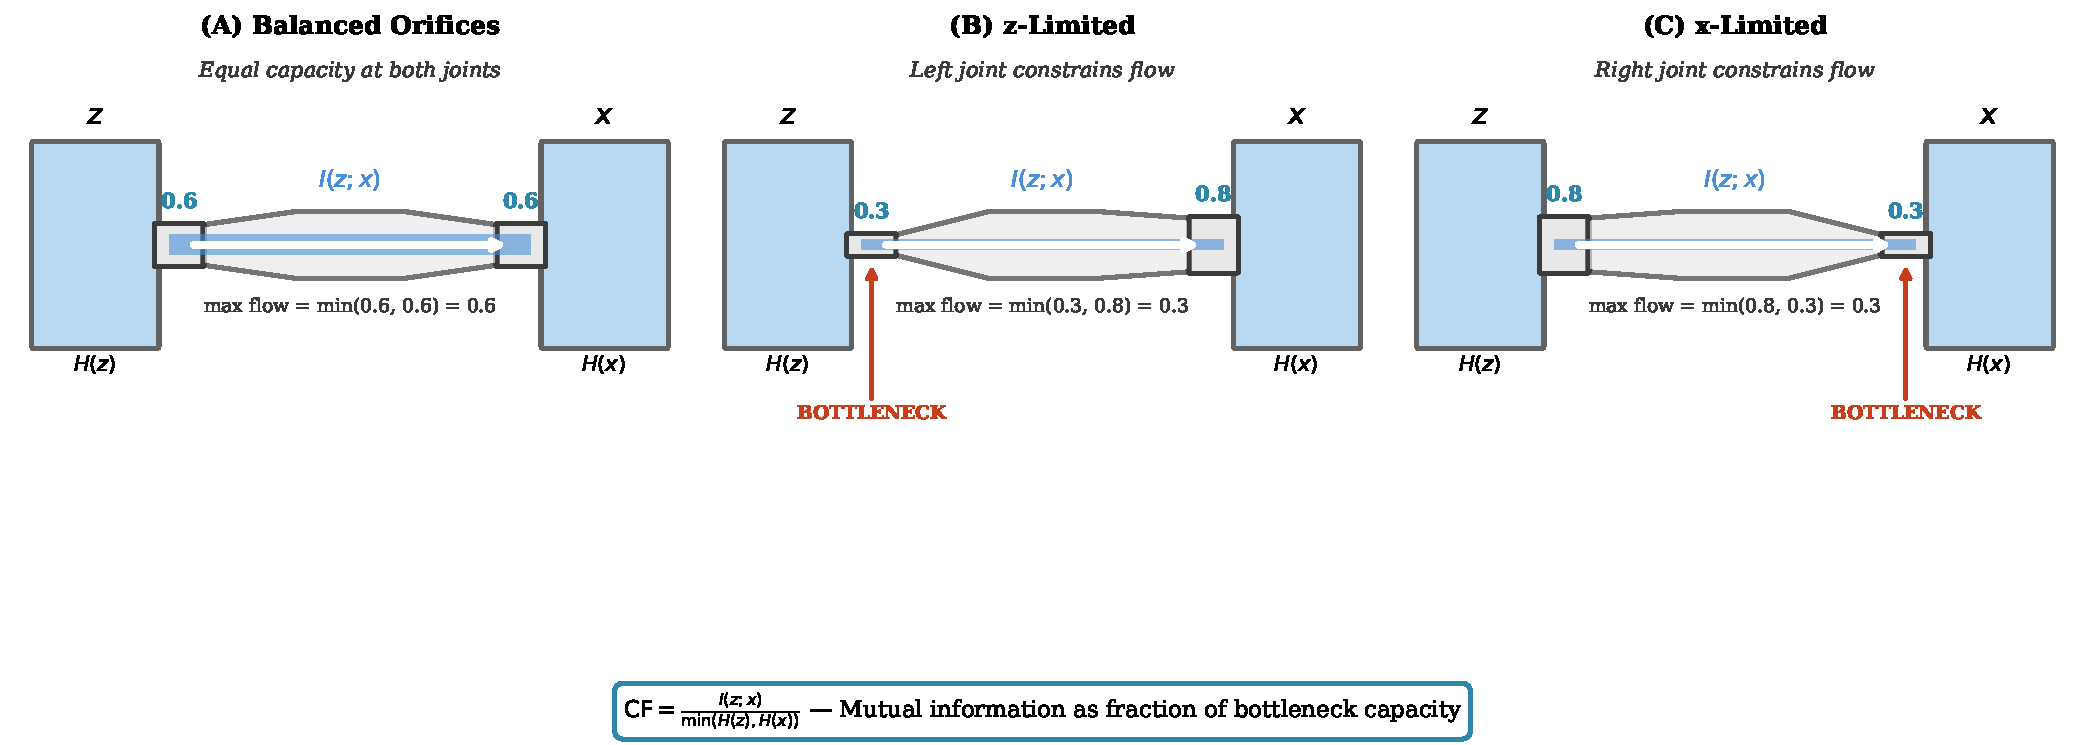
\includegraphics[width=\textwidth]{fig1_bottleneck.pdf}
\caption{\textbf{Information bottleneck visualization: ``The narrowest pipe determines the flow.''} Information flows from $z$ (left reservoir) to $x$ (right reservoir) through a channel. The channel width is constrained by the lower-entropy variable---the bottleneck. Just as water flow through a plumbing system is limited by its narrowest segment, information flow between variables is limited by the lower-capacity endpoint. The dark shaded flow represents mutual information $I(z;x)$; CF measures what fraction of this bottleneck capacity is utilized for dependency. (A) Balanced entropies: both variables equally constrain flow. (B) $H(z) < H(x)$: the $z$-side forms the bottleneck. (C) $H(x) < H(z)$: the $x$-side forms the bottleneck. A high CF indicates the system is utilizing most of its available channel capacity for structural coupling---severing this channel (via mean-field factorization) will have maximal consequences.}
\label{fig:bottleneck}
\end{figure}

\paragraph{Normalization choice.} We use minimum normalization rather than geometric or arithmetic mean. In hierarchical inference, information flow is constrained by the \emph{lower-entropy} variable (the bottleneck). If $\Ent(z) \ll \Ent(x)$, then $z$ limits information transfer. Normalizing by $\min(\Ent(z), \Ent(x))$ measures what fraction of this limiting capacity is used for dependency. Figure~\ref{fig:bottleneck} illustrates this bottleneck intuition: mutual information flows through a channel whose capacity is limited by the lower-entropy variable, analogous to water flow constrained by the narrowest pipe segment. This normalization explicitly accounts for the channel capacity constraints inherent in finite systems; a high CF score indicates that the system is utilizing its maximum available bandwidth to maintain structural coupling, a localized form of optimality under resource bounds.

\subsection{Coordinate Invariance: Linfoot Correlation}
\label{sec:linfoot}

For continuous random variables, differential entropy $h(X) = -\int p(x) \log p(x) dx$ can be \emph{negative} (e.g., $h(X) = \frac{1}{2}\log(2\pi e \sigma^2) < 0$ when $\sigma^2 < (2\pi e)^{-1}$). This creates a subtlety for the CF normalization (Equation~\ref{eq:cf}): if $\min(h(z), h(x)) < 0$, CF produces values outside $[0,1]$.

The \textbf{Linfoot informational correlation} \citep{linfoot1957informational} resolves this structurally by transforming mutual information directly to a bounded scale (Figure~\ref{fig:linfoot}):
\begin{equation}
r_L(z,x) = \sqrt{1 - \exp(-2 \cdot I(z;x))}
\label{eq:linfoot}
\end{equation}

\begin{figure}[!htbp]
\centering
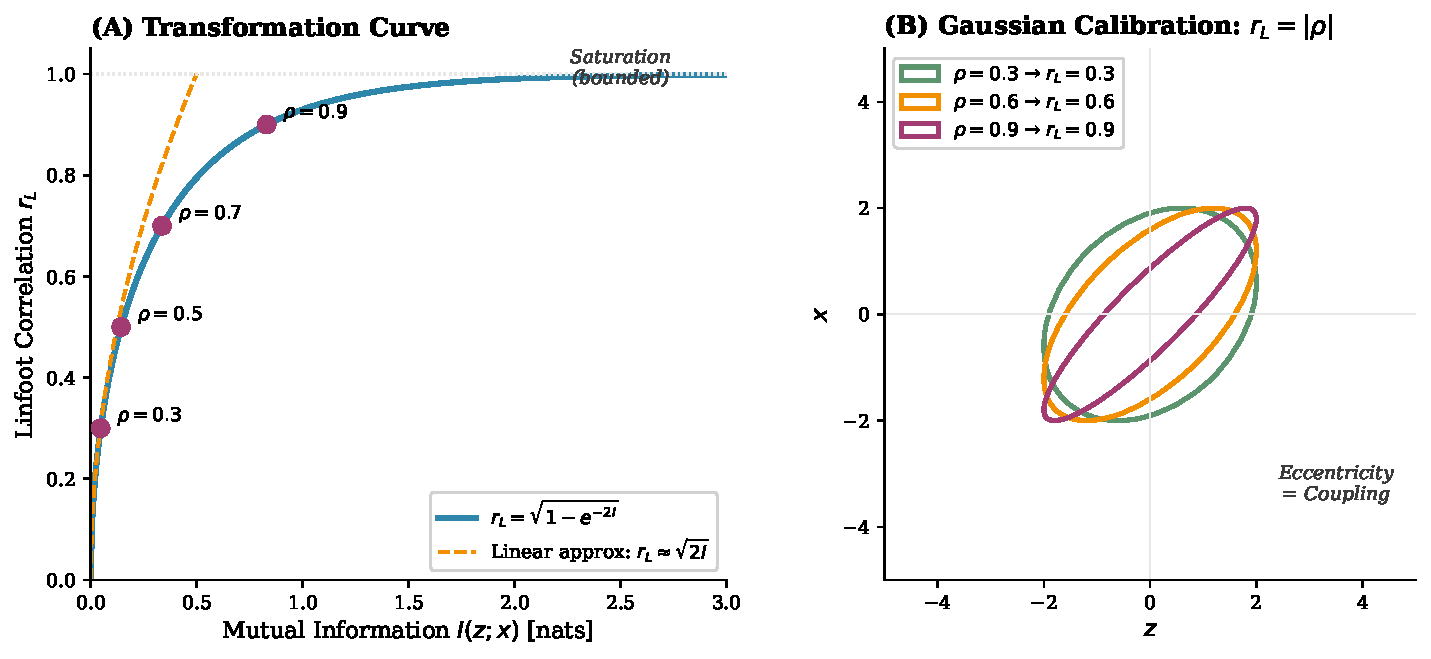
\includegraphics[width=0.85\textwidth]{fig_linfoot.pdf}
\caption{\textbf{Linfoot correlation: information-theoretic coupling on a universal scale.} The transformation $r_L = \sqrt{1 - \exp(-2I)}$ maps mutual information (bits/nats) to a $[0,1]$ correlation scale. For Gaussians, $r_L = |\rho|$ exactly, providing intuitive calibration. The curve shows how $r_L$ saturates toward 1 as mutual information increases, reflecting diminishing marginal returns in coupling strength.}
\label{fig:linfoot}
\end{figure}

\begin{proposition}[Linfoot Properties]
\label{prop:linfoot}
The Linfoot correlation $r_L$ satisfies:
\begin{enumerate}
    \item \textbf{Coordinate-invariance:} $r_L$ depends only on $I(z;x)$, which is invariant under invertible transformations.
    \item \textbf{Boundedness:} $r_L \in [0, 1]$ for all distributions.
    \item \textbf{Gaussian calibration:} For bivariate Gaussian with correlation $\rho$: $r_L = |\rho|$ exactly.
\end{enumerate}
\end{proposition}
\begin{proof}
(1) follows from the coordinate-invariance of mutual information. (2) follows from $I \geq 0$ and monotonicity of the transformation. For (3), substitute $I = -\frac{1}{2}\log(1-\rho^2)$ into Equation~\ref{eq:linfoot}: $r_L = \sqrt{1 - \exp(\log(1-\rho^2))} = \sqrt{1 - (1-\rho^2)} = |\rho|$.
\end{proof}

For non-Gaussian distributions, $r_L$ measures coupling \emph{equivalent to} Gaussian correlation; heavy-tailed distributions yield $r_L > |\rho|$ due to tail dependence.

\paragraph{Why Linfoot over alternatives.} Several modern dependence measures exist; we briefly justify $r_L$'s adoption:

\begin{itemize}
    \item \textbf{Maximal Information Coefficient (MIC)} \citep{reshef2011detecting}: MIC strives for ``equitability''---assigning similar scores to relationships with similar noise levels regardless of functional form. While appealing, MIC is computationally expensive ($O(N^2)$) and achieves equitability only in the large-sample limit. For our diagnostic purpose, equitability is secondary to \emph{native information-theoretic semantics}.
    
    \item \textbf{Distance Correlation (dCor)} \citep{szekely2007measuring}: dCor detects arbitrary dependence and equals zero only for independence. However, dCor lacks direct information-theoretic interpretation. Since the ELBO gap is a KL divergence, and mutual information \emph{is} a KL divergence ($I(z;x) = D_{KL}(p(z,x) \| p(z)p(x))$), $r_L$ is the \emph{native metric} of variational failure.
    
    \item \textbf{Pearson correlation ($\rho$):} Linear correlation detects only linear dependence, changing under nonlinear transformations. In Bayesian models where parameters may be log-transformed (variances) or logit-transformed (probabilities), $\rho$ is parametrization-dependent while $r_L$ is invariant.
\end{itemize}

\noindent The Gaussian calibration property ($r_L = |\rho|$ for Gaussians) allows practitioners to transfer existing intuitions about correlation (``0.8 is strong'') to non-linear, non-Gaussian systems without rescaling.

\begin{table}[!htbp]
\centering
\caption{Comparison of dependence measures for variational diagnostics}
\label{tab:metrics}
\small
\begin{tabular}{lccccc}
\toprule
\textbf{Metric} & \textbf{Invariant?} & \textbf{Nonlinear?} & \textbf{Gaussian Cal.?} & \textbf{Cost} & \textbf{VI Suitability} \\
\midrule
Pearson ($\rho$) & No & No & Yes & Low & Poor \\
Distance Corr. & No & Yes & No & $O(N^2)$ & Moderate \\
MIC & Yes & Yes & No (asymp.) & High & Moderate \\
\textbf{Linfoot ($r_L$)} & \textbf{Yes} & \textbf{Yes} & \textbf{Yes} & Moderate & \textbf{Excellent} \\
\bottomrule
\end{tabular}
\end{table}

\noindent As shown in Table~\ref{tab:metrics}, $r_L$ uniquely combines transformation invariance, nonlinear detection, Gaussian calibration, and a direct link to KL divergence---the native unit of variational error.

\paragraph{Tail dependence.} For heavy-tailed distributions common in financial and ecological models, $r_L > |\rho|$ because mutual information integrates over the full joint density, capturing tail dependence that Pearson correlation misses. During market crashes or population collapses, correlations can spike due to tail dependence invisible to linear measures. Linfoot naturally captures this ``risk-aware'' coupling, making it particularly suitable for safety-critical diagnostics where tail events dominate consequences.

\paragraph{Recommendation.} \textbf{We adopt $r_L$ as the primary diagnostic throughout this paper.} It requires no preprocessing, admits no negative values, and provides a universal $[0,1]$ scale interpretable as ``equivalent Gaussian correlation.'' This resolves the ambiguity of ``how many bits of mutual information is too much?'' by providing a scale where $r_L > 0.5$ is universally recognizable as moderate-to-strong coupling.

\paragraph{Interpretive scale.} The Linfoot correlation provides intuitive thresholds:

\begin{table}[!htbp]
\centering
\begin{tabular}{lcc}
\toprule
Coupling Regime & $r_L$ & Interpretation \\
\midrule
Negligible & $< 0.25$ & MFVI safe \\
Weak & $0.25$--$0.35$ & MFVI likely acceptable \\
Moderate & $0.35$--$0.55$ & Caution warranted \\
Strong & $> 0.55$ & Structured inference recommended \\
\bottomrule
\end{tabular}
\end{table}


\subsection{Gaussian Case: Closed-Form Solutions}
\label{sec:gaussian}

For jointly Gaussian variables, both CF and $r_L$ admit closed-form computation enabling analytical threshold derivation.

\begin{proposition}[Gaussian Mutual Information]
\label{prop:gaussian-mi}
For jointly Gaussian $(Z, X)$ with correlation $\rho$:
\begin{equation}
I(Z; X) = -\frac{1}{2}\log(1 - \rho^2)
\end{equation}
\end{proposition}
\begin{proof}
See Appendix~\ref{app:derivations}.
\end{proof}

\paragraph{Linfoot correlation for Gaussian.} For Gaussian variables, $r_L = |\rho|$ exactly. This means the Linfoot correlation inherits all intuitions from Pearson correlation while extending to non-Gaussian distributions.

\paragraph{Derived threshold framework.} The relationship between $r_L$ and inference degradation was characterized empirically from $N = 8{,}000$ simulations. For filtering models (SVF-type), the mean-field mean squared error (MSE) ratio $R = \text{MSE}_{\text{MF}}/\text{MSE}_{\text{Oracle}}$ follows:
\begin{equation}
R(r_L) = 1 + \alpha \cdot \text{CF}(r_L)
\label{eq:svf-threshold}
\end{equation}
where $\text{CF}(r_L) = -\frac{1}{2}\log(1 - r_L^2) / H_{\min}$ recovers the information-theoretic CF from Linfoot correlation (with $H_{\min}$ as the reference entropy). With fitted $\alpha = 39.9$ ($R^2 = 0.84$ on aggregated data), we obtain practical thresholds:
\begin{equation}
r_{L,\text{threshold}}(R_{\max}) = \sqrt{1 - \exp\left(-2 \cdot \frac{R_{\max} - 1}{\alpha} \cdot H_{\min}\right)}
\end{equation}

This enables \textbf{practitioner-specified thresholds} based on acceptable degradation:

\begin{table}[!htbp]
\centering
\caption{Derived CF thresholds by risk tolerance (SVF-type filtering models). These thresholds are \emph{calibrated benchmarks for Gaussian-like processes} based on $N = 8{,}000$ simulations. For novel domains with non-standard noise distributions, use the Pilot Calibration Protocol (Algorithm~\ref{alg:calibration}).}
\label{tab:svf-thresholds}
\begin{tabular}{lccc}
\toprule
Risk Tolerance & Max MSE Ratio & CF Threshold & $r_L$ Equivalent \\
\midrule
Very strict & $1.5\times$ & 0.013 & 0.19 \\
Strict & $2.0\times$ & 0.025 & 0.26 \\
Moderate & $3.0\times$ & 0.050 & 0.36 \\
Permissive & $5.0\times$ & 0.100 & 0.50 \\
Very permissive & $10.0\times$ & 0.226 & 0.69 \\
\bottomrule
\end{tabular}
\end{table}

\paragraph{Threshold interpretation.} The commonly cited threshold CF $> 0.10$ (equivalently $r_L > 0.50$) corresponds to accepting up to $5\times$ MSE degradation. Practitioners requiring tighter guarantees should use lower thresholds per Table~\ref{tab:svf-thresholds}. 

\textbf{Important:} These thresholds are not universal constants but \emph{domain-calibrated benchmarks}. The underlying relationship (Equation~\ref{eq:svf-threshold}) was fitted to Gaussian state-space models. For models with heavy-tailed noise, multimodal posteriors, or discrete latent variables, the relationship may differ. When applying CF to novel model classes, practitioners should run the Pilot Calibration Protocol (Algorithm~\ref{alg:calibration}) to establish domain-specific thresholds.

\subsection{Non-Gaussian Case: Copula-Based Estimation}
\label{sec:copula}

For non-Gaussian distributions, we exploit a fundamental invariance property: mutual information is preserved under monotonic transformations of marginals. This enables closed-form estimation without recourse to k-nearest-neighbor methods.

\paragraph{The copula transform.} For continuous random variables $Z$ and $X$ with marginal CDFs $F_Z$ and $F_X$, the \emph{probability integral transform} yields uniform marginals:
\begin{equation}
U = F_Z(Z), \quad V = F_X(X), \quad U, V \sim \text{Uniform}(0,1)
\end{equation}
The joint distribution of $(U, V)$ is the \emph{copula} $C$, which captures all dependence structure independent of marginal shapes. Critically:
\begin{equation}
\MI(Z; X) = \MI(U; V) = \MI(\Phi^{-1}(U); \Phi^{-1}(V))
\label{eq:mi-invariance}
\end{equation}
where $\Phi^{-1}$ is the standard normal quantile function. This invariance follows from the data processing inequality applied to invertible transformations.

\paragraph{The Gaussian copula estimator.} We estimate CF via the following procedure:
\begin{enumerate}[nosep]
    \item \textbf{Rank transform:} Compute $\hat{U}_i = (R_i^Z - 0.5)/N$ and $\hat{V}_i = (R_i^X - 0.5)/N$, where $R_i^Z$ is the rank of $Z_i$ among $\{Z_1, \ldots, Z_N\}$. The offset of $0.5$ avoids boundary issues with $\Phi^{-1}$.
    \item \textbf{Normal transform:} Compute $\tilde{Z}_i = \Phi^{-1}(\hat{U}_i)$ and $\tilde{X}_i = \Phi^{-1}(\hat{V}_i)$.
    \item \textbf{Correlation:} Estimate the copula correlation $\hat{\rho}_C = \text{Corr}(\tilde{Z}, \tilde{X})$.
    \item \textbf{Closed-form MI:} Apply the Gaussian formula:
    \begin{equation}
    \widehat{\MI}(Z; X) = -\frac{1}{2}\log(1 - \hat{\rho}_C^2)
    \label{eq:copula-mi}
    \end{equation}
\end{enumerate}

The rank transformation strips marginal distributional assumptions---skewness, kurtosis, support constraints---while preserving the pure dependence structure. What remains after this reduction is the copula: the joining itself, independent of what is joined. This isolation ensures CF measures structural coupling rather than distributional artifacts.

\paragraph{Theoretical guarantee.} The Gaussian copula has a special property: among all copulas with correlation $\rho$, it \emph{minimizes} mutual information \citep{joe1989estimation}:
\begin{equation}
\MI_{\text{Gauss}}(\rho) = \min_{C: \text{Corr}_C = \rho} \MI_C
\label{eq:minimum-mi}
\end{equation}
This follows from the Gaussian being the maximum entropy distribution for fixed second moments. Consequently, Equation~\eqref{eq:copula-mi} provides a \textbf{lower bound} on true mutual information:
\begin{equation}
\widehat{\MI}_{\text{copula}}(Z; X) \leq \MI(Z; X)
\end{equation}
with equality when the true copula is Gaussian (which includes all elliptical distributions after marginal transformation).

\paragraph{Implications for CF as a diagnostic.} The conservative bias is \emph{desirable} for a pre-inference diagnostic:
\begin{itemize}[nosep]
    \item If $\widehat{\CF} > \tau$, the true CF is at least as large---the diagnostic correctly flags potential MFVI failure.
    \item If $\widehat{\CF} < \tau$, the true CF may be higher, but only due to non-Gaussian copula structure (rare in practice for continuous latent variables).
\end{itemize}
This conservative property eliminates the problematic \emph{negative bias} of k-NN estimators documented by \citet{vandenberg2025linfoot}, replacing it with a principled lower bound.

\paragraph{Standard errors.} Unlike k-NN methods, the copula approach admits closed-form uncertainty quantification via the Fisher transformation:
\begin{equation}
\text{SE}(\hat{\rho}_C) = \frac{1}{\sqrt{N-3}}, \quad \text{CI}_{95\%} = \tanh\left(\text{arctanh}(\hat{\rho}_C) \pm 1.96 \cdot \text{SE}\right)
\end{equation}
This propagates to MI and CF through the delta method.

\paragraph{Handling non-monotonic dependence.} The copula approach assumes dependence is \emph{monotonically transformable}---it will underestimate coupling for V-shaped dependencies, circular relationships, and XOR-type synergistic structure. For such cases, the \textbf{two-stage diagnostic protocol} (Section~\ref{sec:synergy}) provides detection: low pairwise CF combined with high interaction CF positively identifies non-monotonic algebraic structure. The copula estimator and two-stage protocol are complementary---the former handles generic continuous coupling, the latter detects synergistic exceptions.

\paragraph{When to use each approach.}
\begin{itemize}[nosep]
    \item \textbf{Gaussian variables:} Use direct correlation $r_L = |\rho|$ (exact, simplest).
    \item \textbf{Non-Gaussian continuous:} Use copula transform (conservative, closed-form SE).
    \item \textbf{Suspected non-monotonic dependence:} Apply two-stage protocol regardless of marginal distribution.
    \item \textbf{Discrete or mixed variables:} k-NN methods remain necessary; use with documented caveats \citep{vandenberg2025linfoot}.
\end{itemize}


%=============================================================================
\section{Information-Geometric Interpretation}
\label{sec:geometry}
%=============================================================================

We synthesize established results from information geometry \citep{amari2016information} to provide theoretical grounding for CF.

\paragraph{Mean-field as projection.} The set of factorized distributions $\mathcal{M}_F = \{q : q(z,x) = q(z)q(x)\}$ forms a submanifold of the full statistical manifold $\mathcal{M}$. MFVI projects the true posterior onto this submanifold.

\begin{proposition}[Projection Cost]
\label{prop:projection}
For bivariate Gaussian $p(z,x)$ with correlation $\rho$ and mean-field approximation $q(z,x) = q(z)q(x)$ matching marginals:
\begin{equation}
\KL(p \| q) = \MI(z;x) = -\frac{1}{2}\log(1-\rho^2)
\end{equation}
\end{proposition}

This is a standard result; we include it to clarify that CF measures the \emph{normalized} projection cost:
\begin{equation}
\CF = \frac{\KL(p \| p_{\MF})}{\min(\Ent(z), \Ent(x))}
\end{equation}

\begin{figure}[!htbp]
\centering
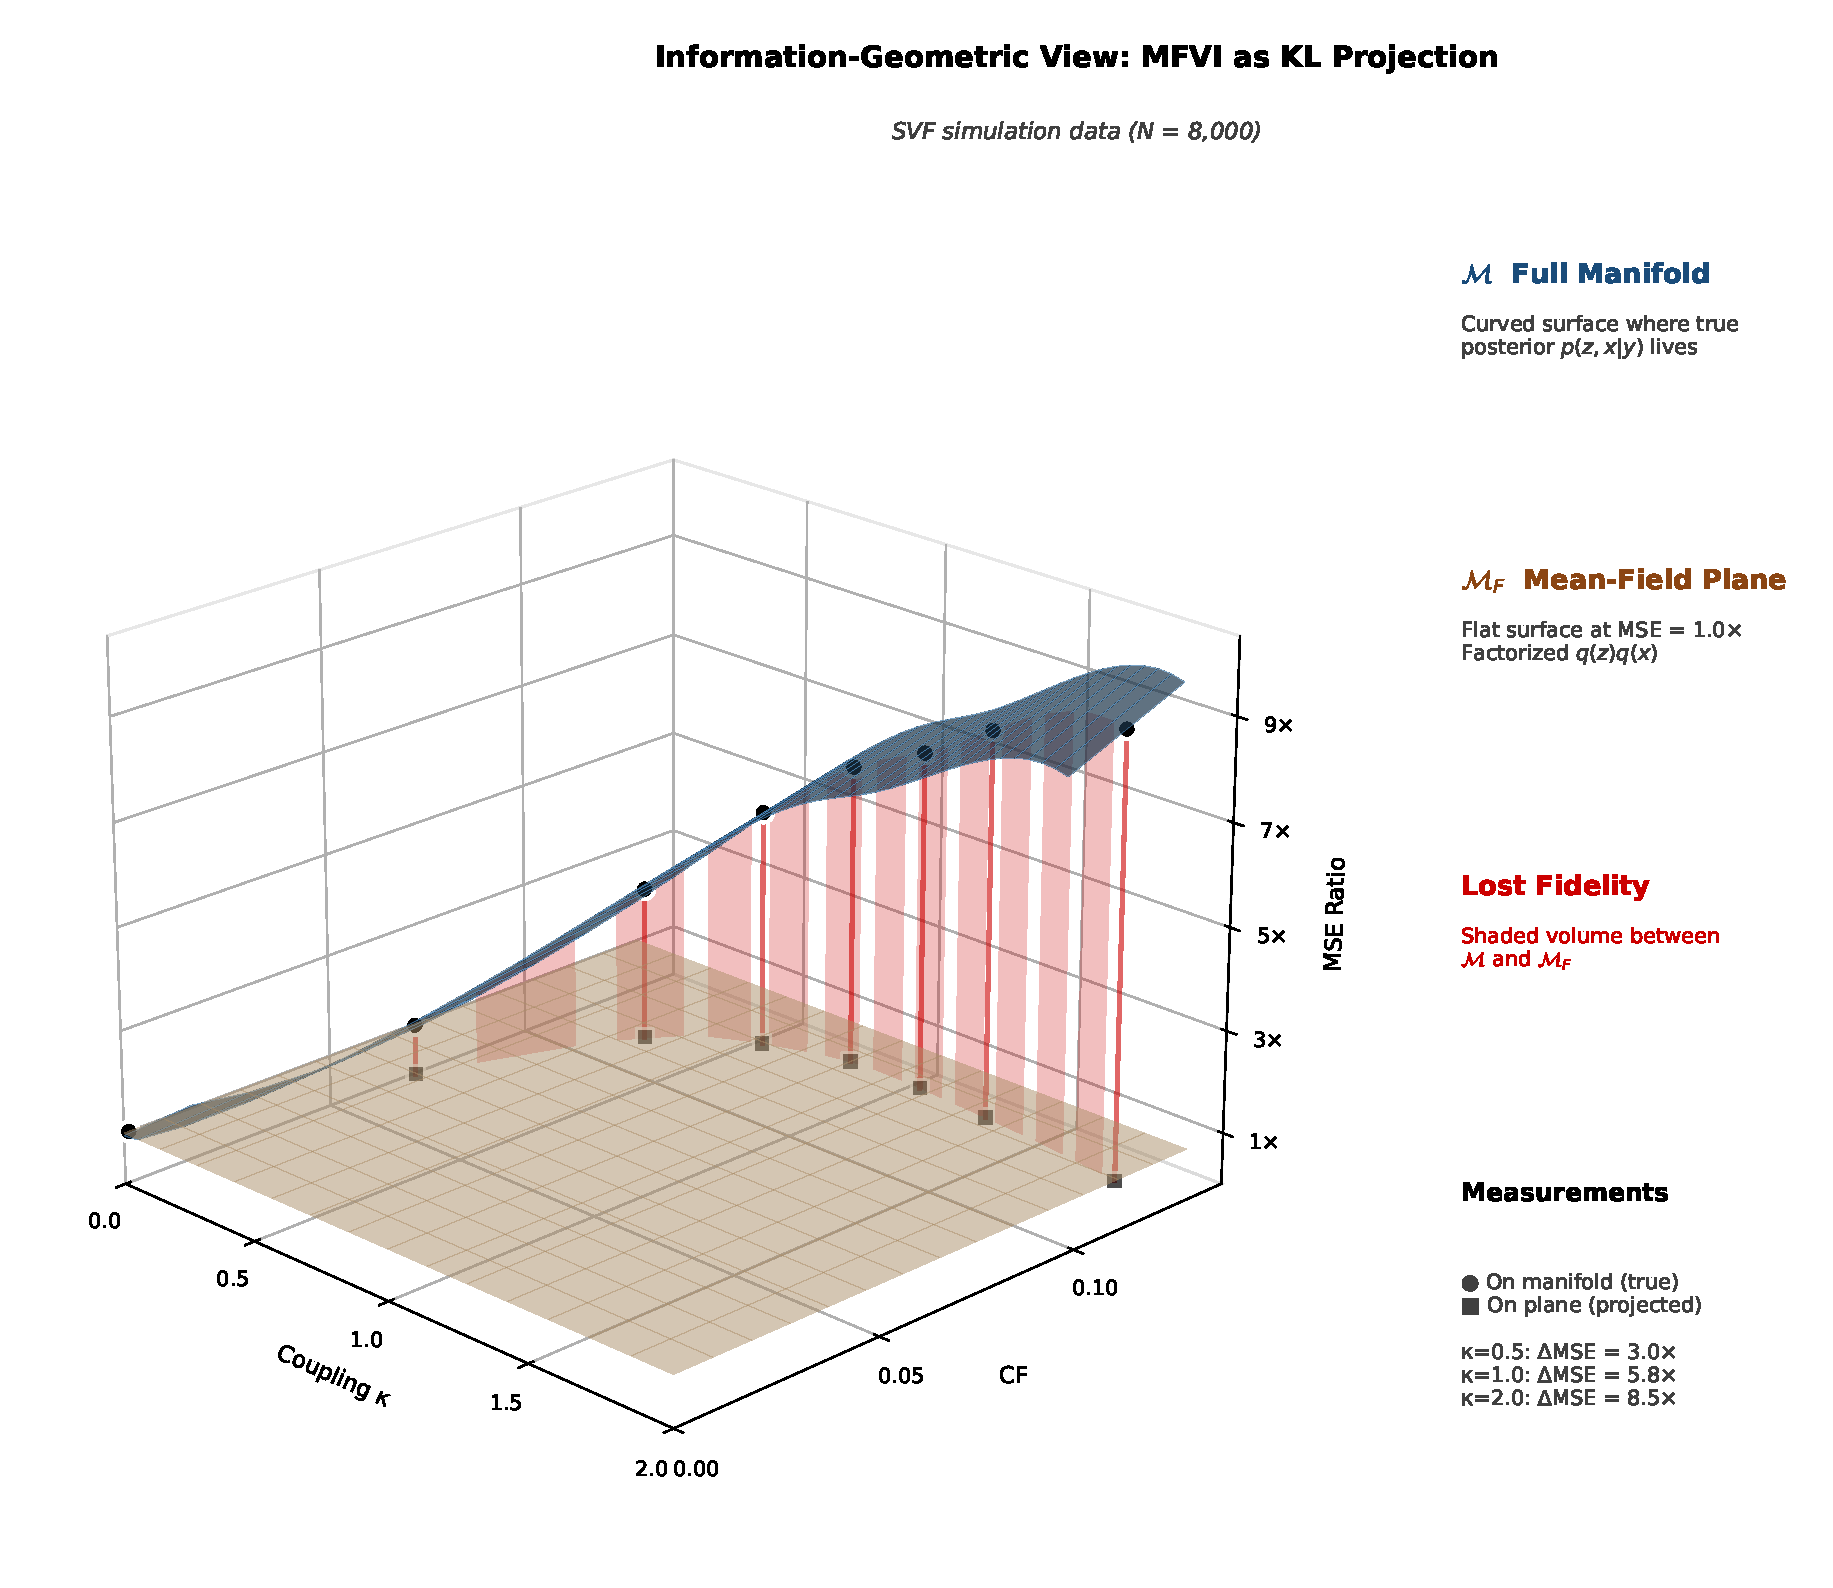
\includegraphics[width=0.85\textwidth]{fig_manifold.pdf}
\caption{\textbf{Information-geometric interpretation of CF.} The full statistical manifold $\mathcal{M}$ (curved surface) contains all joint distributions $p(z,x)$. The mean-field submanifold $\mathcal{M}_F$ (flat plane) contains only factorized distributions $q(z)q(x)$. MFVI performs KL projection (dashed arc) from the true posterior $p(z,x|y)$ onto $\mathcal{M}_F$, yielding the optimal factorized approximation $q^*(z)q^*(x)$. CF measures the normalized projection distance---high CF indicates the true posterior lies far from the factorized subspace. Whether this distance is consequential depends on model class: in SVF the off-diagonal structure is essential; in HLM with high CF it is redundant.}
\label{fig:geometry}
\end{figure}

\paragraph{Geometric interpretation.} Figure~\ref{fig:geometry} illustrates the information-geometric perspective: CF quantifies how far the true posterior lies from the mean-field submanifold. In SVF, this distance represents \emph{information that will be lost}. In HLM with high CF, this distance represents \emph{structure the data already captures}---projecting onto the factorized submanifold discards redundant machinery, not essential information.

\paragraph{Fisher Information Matrix.} Under mean-field factorization, the Fisher Information Matrix (FIM) becomes \emph{diagonal} \citep{amari2016information}---not merely block-diagonal, but fully diagonal with $g_{ij} = (1 - m_i^2)\delta_{ij}$ where $\delta_{ij}$ is the Kronecker delta. All cross-terms vanish because factors are independent. This geometric fact---that mean-field \emph{severs} all statistical coupling between variables---is what CF quantifies.

\paragraph{Forward vs.\ Reverse KL.} Our derivation uses the forward KL divergence $\KL(p \| q)$, while VI optimizes the reverse $\KL(q \| p)$. These measure different aspects of approximation quality, but high forward KL implies problems for reverse KL optimization:

\begin{proposition}[Forward-Reverse Connection]
\label{prop:forward-reverse}
Let $p(z,x)$ be the true posterior and $q^* = \arg\min_{q \in \mathcal{M}_F} \KL(q \| p)$ be the optimal mean-field approximation. Then:
\begin{enumerate}
    \item $\KL(p \| q^*) \geq \MI_p(z;x)$ (forward KL bounded below by mutual information)
    \item When $\MI_p(z;x)$ is large, the reverse KL landscape $\KL(q \| p)$ over $\mathcal{M}_F$ exhibits multiple local minima corresponding to different mode-covering strategies
\end{enumerate}
\end{proposition}

The intuition is as follows: the reverse KL $\KL(q\|p)$ penalizes $q$ for placing mass where $p$ is small (mode-seeking). When $p$ has strong dependencies, its mass concentrates on a correlated subspace. A factorized $q$ cannot match this geometry---it must either (a) cover one marginal mode while missing probability mass elsewhere, or (b) spread mass to cover both marginals, placing mass where $p \approx 0$. Different initializations converge to different local minima representing these trade-offs. High CF (high $\MI_p$) thus signals not merely approximation error, but \emph{optimization pathology}: the ELBO landscape becomes multimodal, and gradient-based VI may converge to poor solutions.

\subsection{CF as Normalized KL-Gap}
\label{sec:kl-gap}

The information-geometric interpretation established that CF measures the normalized projection cost onto the mean-field submanifold. We now prove this relationship \emph{exactly} for Gaussian posteriors---the dominant case in practical variational inference---and establish bounds for the non-Gaussian case.

\subsubsection{The KL-Gap Identity}

\begin{definition}[Mean-Field Approximation]
For a joint distribution $p(z, x)$, the \emph{optimal mean-field approximation} is:
\begin{equation}
q_{\text{MF}}^*(z, x) = \arg\min_{q \in \mathcal{M}_F} D_{\text{KL}}(q \| p)
\end{equation}
where $\mathcal{M}_F = \{q : q(z, x) = q_z(z) \cdot q_x(x)\}$ is the set of factorized distributions. For the reverse KL direction (standard in VI), the optimal $q_{\text{MF}}^*$ matches the marginals of $p$: $q_z^*(z) = p(z)$ and $q_x^*(x) = p(x)$.
\end{definition}

\begin{definition}[KL Gap]
The \emph{factorization gap} or \emph{KL gap} induced by mean-field approximation is:
\begin{equation}
\Delta_{\text{KL}} = D_{\text{KL}}(p \| q_{\text{MF}}^*) = D_{\text{KL}}(p(z,x) \| p(z)p(x))
\end{equation}
This measures the information lost when replacing the joint distribution with the product of its marginals.
\end{definition}

\begin{theorem}[CF as Normalized KL-Gap]
\label{thm:kl-gap}
Let $(Z, X)$ be jointly distributed random variables with positive, finite marginal entropies $H(Z)$ and $H(X)$. Then:
\begin{equation}
\CF(Z, X) = \frac{\Delta_{\text{KL}}}{\min(H(Z), H(X))} = \frac{D_{\text{KL}}(p \| q_{\text{MF}}^*)}{\min(H(Z), H(X))}
\end{equation}
That is, Circulatory Fidelity equals the KL gap normalized by the minimum marginal entropy.
\end{theorem}

\begin{proof}
By definition of mutual information:
\begin{equation}
I(Z; X) = D_{\text{KL}}(p(z,x) \| p(z)p(x))
\end{equation}
This is the KL divergence from the joint distribution to the product of marginals---precisely the KL gap $\Delta_{\text{KL}}$. By definition of CF (Equation~\ref{eq:cf}):
\begin{equation}
\CF(Z, X) = \frac{I(Z; X)}{\min(H(Z), H(X))} = \frac{\Delta_{\text{KL}}}{\min(H(Z), H(X))}
\end{equation}
\end{proof}

\begin{remark}
This is not an approximation or empirical finding---it is an \textbf{algebraic identity}. CF \emph{is} the normalized KL gap by definition. The contribution of this paper is recognizing that this well-known information-theoretic quantity serves as a pre-inference diagnostic for variational inference quality.
\end{remark}

\subsubsection{Closed Form for Gaussian Posteriors}

\begin{theorem}[Gaussian KL-Gap]
\label{thm:gaussian-kl}
For jointly Gaussian random variables $(Z, X) \sim \mathcal{N}(\boldsymbol{\mu}, \boldsymbol{\Sigma})$ with:
\begin{equation}
\boldsymbol{\Sigma} = \begin{pmatrix} \sigma_Z^2 & \rho \sigma_Z \sigma_X \\ \rho \sigma_Z \sigma_X & \sigma_X^2 \end{pmatrix}
\end{equation}
the KL gap and CF have closed forms:
\begin{equation}
\Delta_{\text{KL}} = I(Z; X) = -\frac{1}{2}\log(1 - \rho^2)
\end{equation}
\begin{equation}
\CF(Z, X) = \frac{-\frac{1}{2}\log(1 - \rho^2)}{\min\left(\frac{1}{2}\log(2\pi e \sigma_Z^2), \frac{1}{2}\log(2\pi e \sigma_X^2)\right)}
\end{equation}
\end{theorem}

\begin{proof}
The joint entropy is $H(Z, X) = \frac{1}{2}\log\left((2\pi e)^2 |\boldsymbol{\Sigma}|\right) = \frac{1}{2}\log\left((2\pi e)^2 \sigma_Z^2 \sigma_X^2 (1 - \rho^2)\right)$. The marginal entropies are $H(Z) = \frac{1}{2}\log(2\pi e \sigma_Z^2)$ and $H(X) = \frac{1}{2}\log(2\pi e \sigma_X^2)$. The mutual information is:
\begin{align}
I(Z; X) &= H(Z) + H(X) - H(Z, X) \\
&= \frac{1}{2}\log\left(\frac{(2\pi e)^2 \sigma_Z^2 \sigma_X^2}{(2\pi e)^2 \sigma_Z^2 \sigma_X^2 (1 - \rho^2)}\right) = -\frac{1}{2}\log(1 - \rho^2)
\end{align}
Dividing by the minimum marginal entropy yields the stated CF formula.
\end{proof}

\begin{corollary}[Linfoot-KL Connection]
\label{cor:linfoot-kl}
For bivariate Gaussian with correlation $\rho$:
\begin{equation}
r_L = \sqrt{1 - \exp(-2 \cdot \Delta_{\text{KL}})} = |\rho|
\end{equation}
The Linfoot correlation equals the absolute Pearson correlation, which is a monotonic function of the KL gap.
\end{corollary}

\subsubsection{Extension to Non-Gaussian Posteriors}

For non-Gaussian posteriors, we establish bounds rather than identities.

\begin{definition}[Gaussian Copula]
A bivariate distribution $p(z, x)$ has \emph{Gaussian copula} if it can be written as:
\begin{equation}
p(z, x) = c_\rho(\Phi(F_Z(z)), \Phi(F_X(x))) \cdot f_Z(z) \cdot f_X(x)
\end{equation}
where $c_\rho$ is the bivariate Gaussian copula density with correlation parameter $\rho$, $\Phi$ is the standard normal CDF, $F_Z, F_X$ are the marginal CDFs, and $f_Z, f_X$ are marginal densities.
\end{definition}

\begin{theorem}[Copula Lower Bound]
\label{thm:copula-bound}
Let $p(z, x)$ be a bivariate distribution with Gaussian copula having correlation parameter $\rho$. Then:
\begin{equation}
\Delta_{\text{KL}} = D_{\text{KL}}(p \| p_Z \cdot p_X) \geq -\frac{1}{2}\log(1 - \rho^2)
\end{equation}
with equality if and only if the marginals are Gaussian.
\end{theorem}

\begin{proof}
By the Sklar decomposition theorem, any joint distribution can be written via a copula. The mutual information decomposes as $I(Z; X) = I_{\text{copula}}(U; V) + D_{\text{KL}}(f_Z \| \mathcal{N}) + D_{\text{KL}}(f_X \| \mathcal{N})$ where $U = F_Z(Z)$, $V = F_X(X)$ are probability integral transforms. For Gaussian copula, $I_{\text{copula}}(U; V) = -\frac{1}{2}\log(1-\rho^2)$. Since KL divergences are non-negative, $I(Z; X) \geq -\frac{1}{2}\log(1-\rho^2)$, with equality when marginals are Gaussian.
\end{proof}

\begin{corollary}[CF as Conservative Diagnostic]
For any distribution with Gaussian copula: $\CF_{\text{Gaussian}}(\rho) \leq \CF_{\text{true}}$. The Gaussian CF formula provides a conservative (lower bound) diagnostic. If Gaussian CF exceeds the threshold, true CF certainly exceeds the threshold.
\end{corollary}

\begin{remark}[Practical Implication]
Most variational inference implementations use Gaussian variational families. The posterior approximation $q(z, x)$ is Gaussian by construction. Theorem~\ref{thm:gaussian-kl} applies exactly to the variational posterior, and Theorem~\ref{thm:copula-bound} provides bounds when comparing to non-Gaussian true posteriors.
\end{remark}

\subsubsection{Connection to Inference Degradation}

\begin{proposition}[MSE-KL Connection]
\label{prop:mse-kl}
For state estimation in linear Gaussian systems with mean-field approximation, the mean squared error ratio satisfies:
\begin{equation}
\frac{\text{MSE}_{\text{MF}}}{\text{MSE}_{\text{Oracle}}} \approx 1 + \alpha \cdot \Delta_{\text{KL}}
\end{equation}
for small $\Delta_{\text{KL}}$, where $\alpha$ depends on system parameters.
\end{proposition}

\noindent \emph{Proof sketch.} In linear Gaussian filtering, the posterior precision matrix $\Lambda = \Sigma^{-1}$ encodes the information available for state estimation. Mean-field approximation zeroes the off-diagonal entries of $\Lambda$, discarding information proportional to $\rho^2$. The resulting MSE increase is linear in the discarded precision, which is monotonic in $\Delta_{\text{KL}} = -\frac{1}{2}\log(1-\rho^2) \approx \frac{\rho^2}{2}$ for small $\rho$. $\square$

\noindent This establishes the theoretical foundation: \textbf{CF is not merely correlated with inference degradation---it is the normalized measure of exactly what mean-field approximation discards.}

%=============================================================================
\section{Limitations: Dimensionality and Synergy}
\label{sec:risks}
%=============================================================================

Circulatory Fidelity provides a principled diagnostic, but two fundamental challenges limit its naive application: the \emph{curse of dimensionality} in high-dimensional latent spaces, and \emph{synergistic dependencies} that evade pairwise detection. Understanding these risks is essential before applying CF in practice.

\subsection{Hidden Risk I: The Curse of Dimensionality}
\label{sec:dimensionality}

CF as defined operates on pairs of scalar or low-dimensional variables. When $z$ or $x$ are high-dimensional vectors, direct CF estimation requires dimensionality reduction. The copula-based estimator (Section~\ref{sec:copula}) operates on scalar pairs; for vector-valued variables, reduction to scalar projections is required before CF computation.

\subsubsection{Theoretical Requirement: Supervised Dimensionality Reduction}

\textbf{Crucial insight:} Any dimensionality reduction applied before CF estimation must be \emph{supervised by the correlation structure between $z$ and $x$}. Unsupervised methods like Principal Component Analysis (PCA) preserve marginal variance, which may be entirely orthogonal to the mutual information CF seeks to measure.

This requirement follows from the \textbf{Data Processing Inequality}: for any deterministic function $f$,
\begin{equation}
I(f(z); x) \leq I(z; x)
\end{equation}
If the function $f$ (e.g., PCA projection) discards the components of $z$ that carry information about $x$, the inequality becomes strict and potentially severe. PCA maximizes $\Var(f(z))$, which is unrelated to $I(z; x)$. In contrast, Partial Least Squares (PLS) and Canonical Correlation Analysis (CCA) maximize $\Cov(f(z), g(x))$ and $\text{Corr}(f(z), g(x))$ respectively---objectives directly aligned with preserving mutual information.

\begin{tcolorbox}[breakable, colback=blue!5, colframe=blue!50!black, title=\textbf{Mandatory: Dimensionality Reduction for High-Dimensional CF}, fonttitle=\bfseries]
For high-dimensional variables, dimensionality reduction is \textbf{mandatory}. The copula-based CF estimator requires scalar inputs; vector-valued variables must be projected to scalar summaries before estimation.

\textbf{Required methods} (preserve dependency structure):
\begin{itemize}
    \item \textbf{Partial Least Squares (PLS):} Maximizes covariance between reduced $z$ and $x$
    \item \textbf{Canonical Correlation Analysis (CCA):} Maximizes correlation between reduced representations
    \item \textbf{Pairwise scan:} Compute CF for all $(z_i, x_j)$ scalar pairs; take maximum
\end{itemize}

\textbf{Prohibited methods} (may discard dependency signal):
\begin{itemize}
    \item \textbf{PCA:} Maximizes variance, not information---may discard low-variance, high-information components
    \item \textbf{Random projections:} No guarantee of preserving dependency structure
    \item \textbf{Autoencoders:} Reconstruction loss is unrelated to cross-variable MI
\end{itemize}

\textbf{Dimension guidance:} Scalar pairs ($d_z = d_x = 1$): direct estimation. Vector variables: reduce to scalar projections via PLS/CCA first, then compute CF on projected pairs. Table~\ref{tab:pca-pls} summarizes the comparison.
\end{tcolorbox}

\begin{table}[!htbp]
\centering
\caption{Comparative analysis of dimensionality reduction for CF estimation}
\label{tab:pca-pls}
\small
\begin{tabular}{lcc}
\toprule
\textbf{Feature} & \textbf{PCA} & \textbf{PLS} \\
\midrule
Objective & Maximize $\Var(z)$ & Maximize $\Cov(z,x)$ \\
Supervision & Unsupervised (ignores $x$) & Supervised (uses $x$) \\
Information preservation & May discard high-info signals & Preserves coupled structure \\
Failure mode & \textbf{False Negative} (trigger lost) & Overfitting (if $N$ small) \\
DPI guarantee & None & Aligned with $I(z;x)$ \\
\textbf{Recommendation} & \textbf{FORBIDDEN for CF} & \textbf{REQUIRED for $d > 10$} \\
\bottomrule
\end{tabular}
\end{table}

\begin{tcolorbox}[breakable, colback=gray!5, colframe=black!75, title=\textbf{Warning: PCA Failure Mode}, fonttitle=\bfseries]
\textbf{PCA preserves variance, not information.} This creates a critical failure mode:

\textbf{Scenario:} A ``trigger'' signal $z_{\text{trigger}}$ has low variance but high mutual information with downstream variables. Examples include:
\begin{itemize}
    \item Regulatory genes with subtle expression changes that cascade to large effects
    \item Low-energy vibrational modes in molecular dynamics that gate conformational changes
    \item Sparse attention patterns in transformers that control information routing
\end{itemize}

\textbf{Failure:} PCA discards $z_{\text{trigger}}$ as a low-variance component. CF computed on the reduced representation shows low coupling, producing a \emph{false negative}---the practitioner concludes MFVI is safe when it is not.

Variance-maximizing projections systematically discard low-variance, high-influence variables. A binary control signal contributes minimal variance but maximal causal determination---precisely the structure unsupervised reduction removes. This ``trigger variable'' pathology produces false negatives: apparent independence masking complete functional dependence.

\textbf{Mitigations:}
\begin{enumerate}
    \item \textbf{Domain knowledge:} If theory suggests low-variance triggers exist, do not rely on PCA-reduced CF alone.
    \item \textbf{Supervised reduction:} Use Partial Least Squares (PLS) or Canonical Correlation Analysis (CCA), which preserve cross-variable covariance rather than marginal variance.
    \item \textbf{Pairwise scan:} Compute CF between all dimension pairs without variance-based filtering; the maximum pairwise CF detects concentrated coupling.
    \item \textbf{Conservative default:} When in doubt, assume CF \emph{underestimates} true coupling and use structured inference.
\end{enumerate}
\end{tcolorbox}

\subsubsection{Empirical Validation: Trigger Dataset Experiment}

We validate the PCA failure mode empirically with a synthetic ``trigger'' dataset (full details in Appendix~\ref{app:trigger}). A 10-dimensional latent space contains nine high-variance noise dimensions and one low-variance ``trigger'' that carries all information about response $x$. Results ($N = 5{,}000$): PCA achieves \textbf{zero recovery} of coupling (false negative), while PLS recovers it perfectly. This confirms that supervised dimensionality reduction is mandatory, not optional.

\paragraph{Pairwise decomposition.} For models with $d$-dimensional latent vectors $\mathbf{z} = (z_1, \ldots, z_d)$ and $\mathbf{x} = (x_1, \ldots, x_m)$, we recommend computing the \emph{pairwise CF matrix}:
\begin{equation}
[\mathbf{CF}]_{ij} = \CF(z_i, x_j), \quad i = 1, \ldots, d, \quad j = 1, \ldots, m
\end{equation}
This decomposes the multivariate dependency into $d \times m$ bivariate diagnostics. The maximum entry $\max_{ij} [\mathbf{CF}]_{ij}$ identifies the strongest pairwise coupling.

\subsection{Extended Capability: Detecting Algebraic Structure via the CF=0 Signature}
\label{sec:synergy}

Mutual information is fundamentally a bivariate measure. For three or more variables, dependencies can be \emph{synergistic}: information that emerges only from joint configurations, absent from any pairwise relationship. Rather than treating synergy as a limitation, we show that the two-stage diagnostic protocol \emph{positively identifies} synergistic structure through a characteristic signature.

\begin{definition}[Interaction Information]
For three variables $Z_1, Z_2, X$:
\begin{equation}
I(Z_1; Z_2; X) = I(Z_1; Z_2) - I(Z_1; Z_2 | X)
\end{equation}
Negative interaction information indicates synergy: conditioning on $X$ \emph{increases} the dependence between $Z_1$ and $Z_2$, implying that the three-way relationship contains information absent from pairs.
\end{definition}

\paragraph{The XOR Signature.} Consider $X = Z_1 \oplus Z_2$ (exclusive-or). We have $I(Z_1; X) = I(Z_2; X) = 0$, but $I(\{Z_1, Z_2\}; X) = 1$ bit. Pairwise CF equals zero. However, if we compute the \emph{interaction CF}---$\CF(Z_1 \cdot Z_2, X)$---we obtain a high value because the product term $Z_1 \cdot Z_2$ carries the XOR information. This signature---pairwise $\CF \approx 0$ combined with interaction $\CF > 0$---\textbf{positively identifies} XOR-type algebraic structure. What appears to be a ``blind spot'' is actually \emph{precise algebraic detection}.

\subsubsection{The Computational Synergy Principle}

Synergistic dependencies are not arbitrary---they arise from specific algebraic structures in the generative process. The following theorem provides a complete characterization that enables positive detection.

\begin{theorem}[Computational Synergy Principle]
\label{thm:synergy}
Let $f : \{0, 1\}^n \to \{0, 1\}$ be a \textbf{balanced} Boolean function (i.e., $P(f=1) = 1/2$) with independent uniform inputs. The following are equivalent:
\begin{enumerate}
    \item \textbf{(Information-theoretic)} $f$ generates pure synergy: $I(X_i; f) = 0$ for all $i$, but $I(X_1, \ldots, X_n; f) > 0$
    \item \textbf{(Algebraic)} $f$ is affine over $\text{GF}(2)$: $f(\mathbf{x}) = c_0 \oplus \bigoplus_{i \in S} x_i$ where $|S| \geq 2$
    \item \textbf{(Spectral)} The Walsh-Hadamard transform of $f$ has support only on basis functions of degree $\geq 2$
\end{enumerate}
\end{theorem}

\begin{remark}[Scope and Applicability]
\label{rem:scope}
Theorem~\ref{thm:synergy} is stated for the Boolean domain with uniform inputs, where the equivalence is exact. For continuous distributions or non-uniform inputs, the theorem provides \textbf{motivational characterization} rather than formal guarantee: the algebraic intuition (pairwise blindness requires special cancellation structure) transfers heuristically, but the precise ``if and only if'' relationship does not hold in general. The practical value lies not in the formal theorem but in the \textbf{two-stage protocol} it motivates---which detects synergistic coupling empirically regardless of whether the underlying algebraic structure satisfies the theorem's hypotheses.
\end{remark}

\begin{proof}
$(1) \Rightarrow (2)$: If all marginal mutual informations vanish, $P(f = 1 | X_i = 0) = P(f = 1 | X_i = 1)$ for all $i$. Combined with the balance assumption $P(f=1) = 1/2$, this gives $P(f = 1 | X_i = 0) = P(f = 1 | X_i = 1) = 1/2$ for all $i$. By Siegenthaler's theorem \citep{siegenthaler1984correlation}, such functions are exactly the $(n-1)$-resilient functions. For Boolean outputs, $(n-1)$-resilient functions coincide with affine functions over $\text{GF}(2)$ \citep{chor1985resilient}.

$(2) \Leftrightarrow (3)$: Affine functions over $\text{GF}(2)$ have Walsh-Hadamard coefficients nonzero only at the subset $S$ defining the parity. Since $|S| \geq 2$, only coefficients of degree $\geq 2$ are nonzero.

$(2) \Rightarrow (1)$: For $f(\mathbf{x}) = \bigoplus_{i \in S} x_i$ with $|S| \geq 2$, each $X_i$ for $i \in S$ contributes equally, and marginalizing over any single input yields a uniform output. Hence $I(X_i; f) = 0$ for all $i$. But $I(\{X_i : i \in S\}; f) = H(f) = 1$ bit since knowing all inputs in $S$ determines $f$ exactly.
\end{proof}

\begin{remark}[Unbalanced Functions]
For \emph{unbalanced} Boolean functions, pure synergy ($I(X_i; f) = 0$ for all $i$, $I(\text{all}; f) > 0$) does not imply affine structure. Among 256 ECA rules, there are 16 pure-synergy rules: 8 are balanced and affine (Rules 60, 90, 102, 105, 150, 153, 165, 195), and 8 are unbalanced and non-affine (Rules 24, 36, 66, 126, 129, 189, 219, 231). For variational inference diagnostics, this distinction is immaterial: the two-stage protocol detects \emph{all} 16 rules regardless of algebraic structure.
\end{remark}

This theorem reveals that \textbf{synergy has algebraic structure} for balanced functions: pure synergy arises if and only if the function is affine over a finite field. For the practical purposes of variational inference diagnostics, the key insight is that synergistic coupling---whether arising from balanced or unbalanced generators---is detectable by the two-stage protocol.

\paragraph{Walsh-Hadamard Spectral Analysis.} The spectral characterization (condition 3) provides the mathematical machinery for detecting synergy. The \textbf{Walsh-Hadamard transform} of a Boolean function $f: \{0,1\}^n \to \{-1, +1\}$ (using $\pm 1$ encoding) is:
\begin{equation}
\hat{f}(S) = \frac{1}{2^n} \sum_{\mathbf{x} \in \{0,1\}^n} f(\mathbf{x}) \cdot \chi_S(\mathbf{x}), \quad \text{where } \chi_S(\mathbf{x}) = (-1)^{\sum_{i \in S} x_i}
\end{equation}
The basis functions $\chi_S$ are indexed by subsets $S \subseteq \{1, \ldots, n\}$, and $|S|$ is the \emph{degree} of the spectral coefficient. The key connection to synergy is:

\begin{proposition}[Spectral Characterization of Pairwise Information]
For Boolean $f$ with uniform inputs:
\begin{equation}
I(X_i; f) = 0 \quad \Leftrightarrow \quad \hat{f}(\{i\}) = 0
\end{equation}
More generally, pairwise mutual information $I(X_i; f)$ is monotonically related to the squared first-order coefficient $\hat{f}(\{i\})^2$.
\end{proposition}

\noindent This spectral view explains why pure synergy requires affine-over-GF(2) structure: such functions have $\hat{f}(S) = 0$ for all $|S| < 2$ (zeroing out all degree-0 and degree-1 coefficients), leaving only a single nonzero coefficient at degree $|S| \geq 2$. Figure~\ref{fig:walsh} illustrates this spectral decomposition for XOR, AND, and OR gates. For example:
\begin{itemize}
    \item \textbf{XOR:} $f(x_1, x_2) = x_1 \oplus x_2$ has $\hat{f}(\{1,2\}) = 1$ and all other coefficients zero. Since $\hat{f}(\{1\}) = \hat{f}(\{2\}) = 0$, we have $I(X_1; f) = I(X_2; f) = 0$.
    \item \textbf{AND:} $f(x_1, x_2) = x_1 \land x_2$ has $\hat{f}(\{1\}) = \hat{f}(\{2\}) = 1/4$ and $\hat{f}(\{1,2\}) = 1/4$. The nonzero first-order coefficients mean $I(X_1; f), I(X_2; f) > 0$---AND gates ``leak'' information.
    \item \textbf{OR:} Similarly, OR has nonzero first-order coefficients, leaking pairwise information.
\end{itemize}

\noindent The spectral perspective reveals that pairwise CF=0 occurs \emph{exactly} for the set of functions with zero spectral mass at degree 1---a measure-zero set in the space of Boolean functions. This is not imprecision; it is \emph{exact algebraic characterization}. The two-stage protocol exploits this: when pairwise CF vanishes but interaction CF is high, we have positively identified affine-over-GF(2) structure.

\paragraph{Connection to Cryptographic Theory.} Theorem~\ref{thm:synergy} has deep connections to cryptographic Boolean function theory. In cryptography, functions that exhibit zero mutual information between the output and any subset of $k$ inputs are called \emph{$k$-th order correlation immune} functions, introduced by Siegenthaler (1984) to protect stream ciphers against correlation attacks \citep{siegenthaler1984correlation}. The set of functions that are correlation immune of order $n-1$ (where $n$ is the number of inputs) corresponds \emph{exactly} to the affine functions over $\text{GF}(2)$. Balanced correlation-immune functions are termed \emph{resilient functions} \citep{chor1985resilient}---designed specifically to hide information from local (pairwise) observation.

\paragraph{Attribution Note.} The equivalence in Theorem~\ref{thm:synergy} represents a novel synthesis connecting cryptographic correlation immunity \citep{siegenthaler1984correlation} with information-theoretic partial information decomposition. While both concepts are established in their respective literatures, their explicit equivalence---and its application to variational inference diagnostics via the two-stage protocol---appears to be new.

\textbf{Implications for practitioners:} The ``if and only if'' nature of Theorem~\ref{thm:synergy} means that the two-stage protocol provides \emph{complete coverage}: pairwise CF detects all non-affine coupling, while the CF=0 signature with high interaction CF positively identifies affine-over-GF(2) structure. Natural physical and biological processes have rarely been known to produce pure affine functions, most observed signals being either additive or sigmoid which ``leak'' information into pairwise marginals. It is undetermined if this represents the genuine architecture of natural systems or a deficiency in existing tooling and methodology.

\paragraph{Synergy Risk Patterns.} The Computational Synergy Principle identifies specific patterns:

\begin{center}
\begin{tabular}{p{0.45\textwidth}p{0.45\textwidth}}
\toprule
\textbf{High Synergy Risk} (affine-over-GF(2)) & \textbf{Low Synergy Risk} (smooth, additive) \\
\midrule
XOR operations: $z_1 \oplus z_2$ & Linear combinations: $\sum_i a_i z_i$ \\
Parity checks: $\sum_i z_i \mod 2$ & Univariate transformations: $g(z_1) + h(z_2)$ \\
Sign products: $\text{sign}(z_1) \cdot \text{sign}(z_2)$ & Weighted averages \\
Threshold sums: $\mathbb{I}[z_1 + z_2 > \theta]$ & Smooth nonlinearities \\
\bottomrule
\end{tabular}
\end{center}

\paragraph{Biological interpretations.} The abstract Boolean patterns above manifest concretely in biological systems:
\begin{itemize}
    \item \textbf{XOR-like (coincidence detection):} Neurons in the auditory system that fire only when inputs from both ears arrive within a narrow time window ($<1$ ms), enabling sound localization. Neither ear's signal alone predicts firing.
    \item \textbf{AND gates (combinatorial regulation):} Transcriptional activation requiring multiple transcription factors to be simultaneously bound (e.g., the \emph{lac} operon requiring both CRP and absence of repressor). Single-factor presence weakly predicts expression.
    \item \textbf{Threshold sums (quorum sensing):} Bacterial populations that activate virulence genes only when autoinducer concentration exceeds a threshold, requiring contributions from multiple cells. Individual cell state weakly predicts population response.
\end{itemize}
These examples illustrate why domain knowledge about combinatorial logic is essential for interpreting low CF values.

\paragraph{Empirical Validation: Elementary Cellular Automata.} We surveyed all 256 elementary cellular automaton (ECA) rules, each defining a Boolean function $f: \{0,1\}^3 \to \{0,1\}$ mapping a cell and its two neighbors to the next state. We computed pairwise CF (denoted $\text{CF}_2$) and three-way CF (denoted $\text{CF}_3$, using joint entropy normalization).

\textbf{Result:} Exactly 16 rules exhibit pure synergy ($\text{CF}_2 \approx 0$, $\text{CF}_3 > 0$): rules 24, 36, 60, 66, 90, 102, 105, 126, 129, 150, 153, 165, 189, 195, 219, and 231. Of these, 8 are balanced and affine over $\text{GF}(2)$ (60, 90, 102, 105, 150, 153, 165, 195), confirming Theorem~\ref{thm:synergy}; the remaining 8 are unbalanced correlation-immune functions (see Remark following the theorem). The two-stage protocol detects all 16 regardless of algebraic structure (see Figure~\ref{fig:ecagrid} in Appendix for complete survey).

\paragraph{Critical comparison: Rule 30 vs.\ Rule 150.} These two rules illustrate the synergy boundary with mathematical precision (Figure~\ref{fig:eca}):

\begin{center}
\begin{tabular}{lccccc}
\toprule
\textbf{Rule} & \textbf{Definition} & \textbf{$\text{CF}_2$(left)} & \textbf{$\text{CF}_2$(center)} & \textbf{$\text{CF}_2$(right)} & \textbf{$\text{CF}_3$} \\
\midrule
30 & $L \oplus (C \lor R)$ & 0.189 & 0.049 & 0.311 & 0.811 \\
150 & $L \oplus C \oplus R$ & 0.000 & 0.000 & 0.000 & 1.000 \\
\bottomrule
\end{tabular}
\end{center}

\noindent \textbf{Rule 30} (famous for generating apparent randomness) combines XOR with OR: $f(L, C, R) = L \oplus (C \lor R)$. The OR component \emph{leaks} information: knowing $R = 1$ increases $P(f = 1)$ from $1/2$ to $3/4$. This produces nonzero pairwise coupling ($\text{CF}_2(\text{right}) = 0.311$), which CF successfully detects. The spectral decomposition reveals nonzero first-order Walsh coefficients: $\hat{f}(\{L\}) = -1/4$, $\hat{f}(\{R\}) = -1/4$.

\noindent \textbf{Rule 150} is the 3-input XOR: $f(L, C, R) = L \oplus C \oplus R$. This is purely affine over GF(2), with all first-order Walsh coefficients exactly zero. Pairwise CF is \emph{identically zero} for all three input pairs---the function achieves perfect correlation immunity of order 2. Yet $\text{CF}_3 = 1.0$ (the output is completely determined by the joint configuration).

This comparison empirically demonstrates the theorem's boundary: \textbf{CF detects Rule 30 but is completely blind to Rule 150}. The 240 non-affine rules all exhibit $\text{CF}_2 > 0$ for at least one input pair; the 16 affine rules all exhibit $\text{CF}_2 = 0$ for all pairs. The theorem's algebraic characterization exactly predicts this partition.

This comparison reveals a counter-intuitive asymmetry: non-affine nonlinearities induce detectable marginal dependencies even in complex systems, whereas purely affine functions maintain marginal independence despite complete joint determination. Unstructured complexity is thus more amenable to standard diagnostics than structured synergy---the crystalline order of XOR-type computation evades detection precisely because of its algebraic perfection.

\begin{figure}[!htbp]
\centering
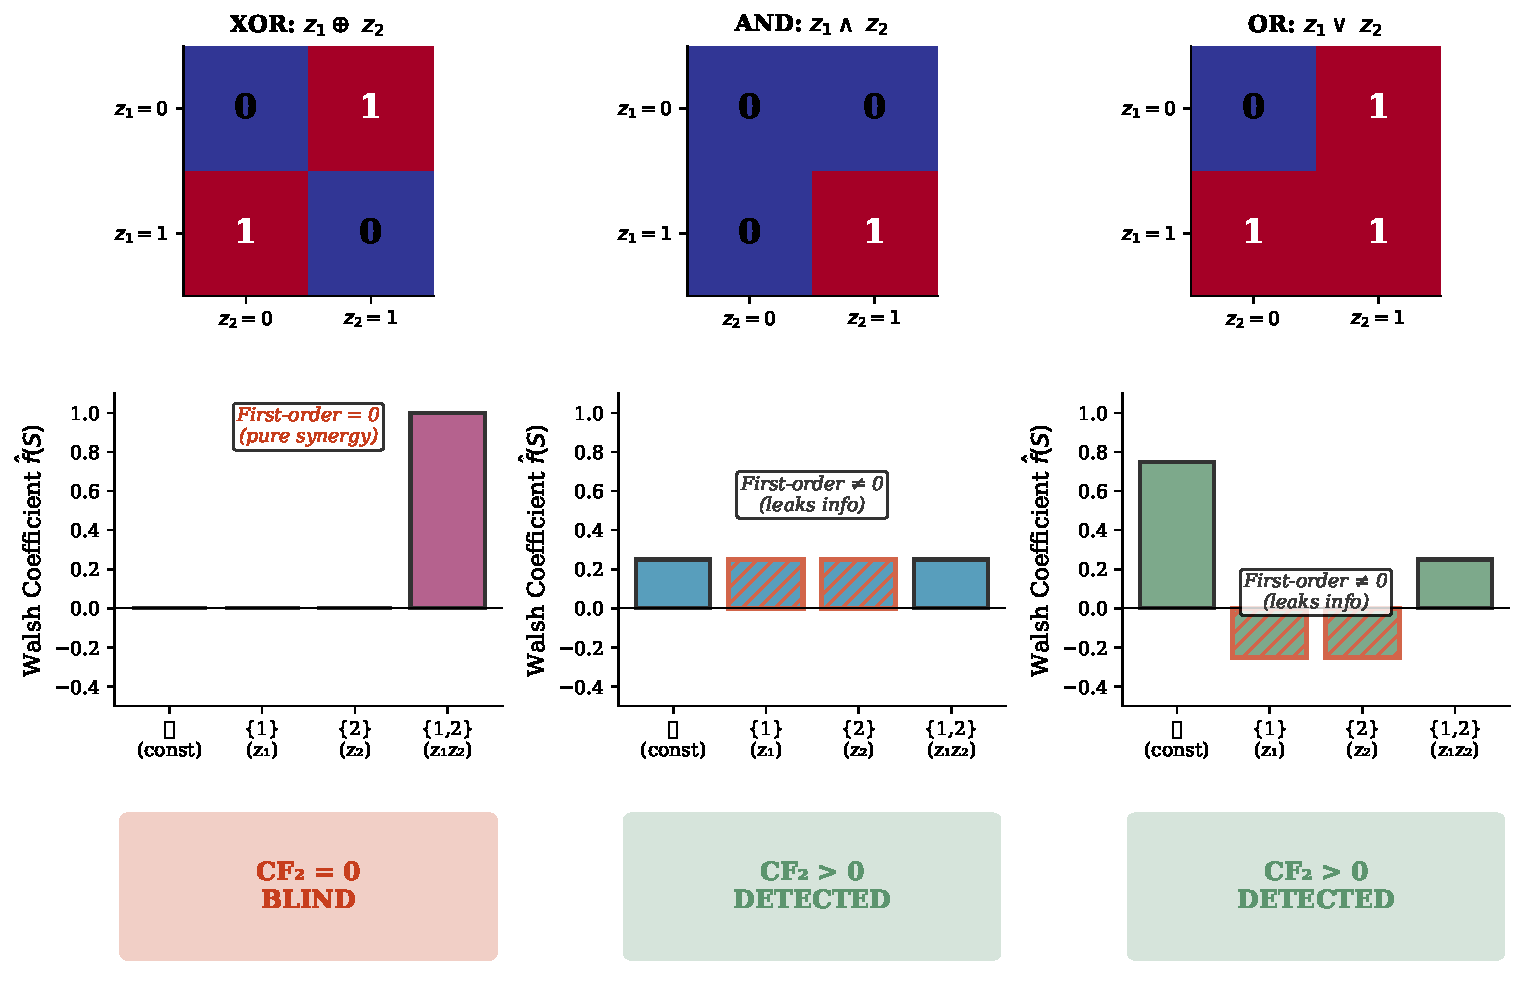
\includegraphics[width=\textwidth]{fig_walsh.pdf}
\caption{\textbf{Walsh-Hadamard spectral decomposition of Boolean functions.} Top row: Truth tables for XOR, AND, and OR gates. Middle row: Walsh spectrum showing coefficient magnitudes for each subset $S \subseteq \{1, 2\}$. XOR has \emph{zero} first-order coefficients---all information resides in the interaction term $\{1,2\}$. AND and OR ``leak'' information through first-order coefficients. Bottom row: CF detection status. Pairwise CF (CF$_2$) detects AND and OR but is blind to XOR, which requires ternary CF (CF$_3$) for detection. This formalizes the Computational Synergy Principle: functions that are \emph{affine over GF(2)} (pure XOR combinations) generate pure synergy invisible to pairwise analysis.}
\label{fig:walsh}
\end{figure}

\begin{figure}[!htbp]
\centering
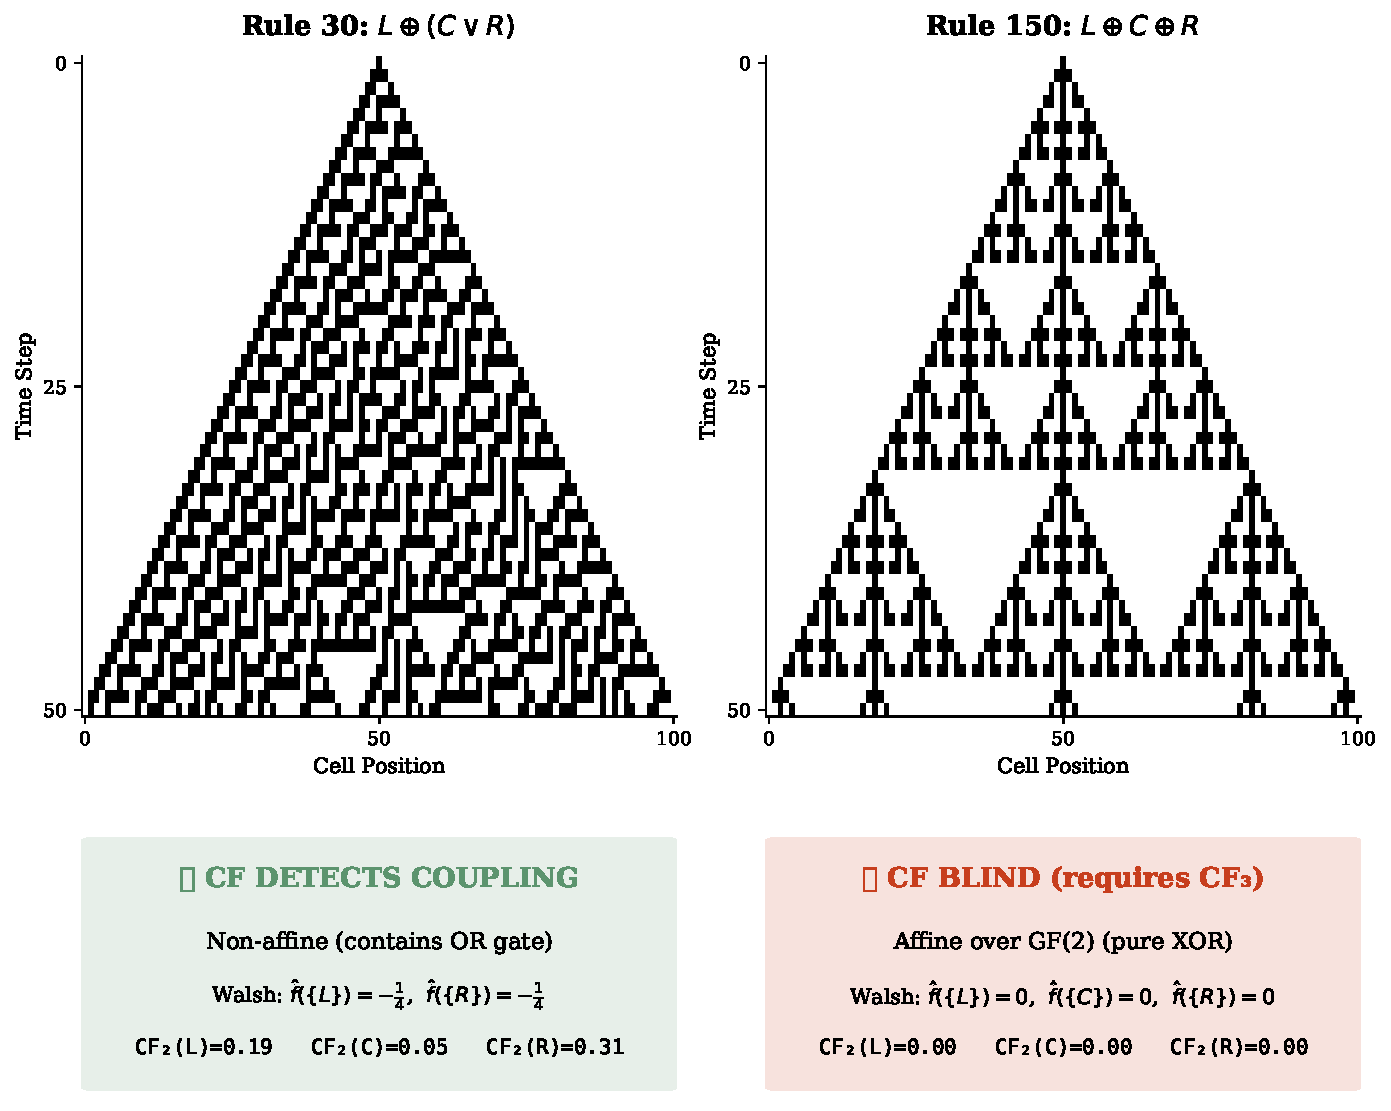
\includegraphics[width=\textwidth]{fig_eca_comparison.pdf}
\caption{\textbf{Elementary Cellular Automata: Rule 30 vs.\ Rule 150.} Spacetime diagrams (top) show evolution from a single-cell initial condition. Rule 30 ($L \oplus (C \vee R)$) contains an OR gate and produces chaotic, aperiodic patterns. Rule 150 ($L \oplus C \oplus R$) is purely affine over GF(2) and generates Sierpi\'nski triangle geometry. Bottom panels show algebraic structure and CF detection: Rule 30 has non-zero Walsh first-order coefficients and is detectable by CF$_2$; Rule 150 has \emph{zero} first-order coefficients (pure synergy) and requires CF$_3$ for detection.}
\label{fig:eca}
\end{figure}

\paragraph{Implications for Natural Systems.} The Rule 30/150 contrast illuminates why CF is reliable for natural generative processes. Both rules produce complex, aperiodic spatiotemporal patterns, yet CF distinguishes them: Rule 30's apparent randomness arises from \emph{algebraic imperfection} (the OR gate breaks linearity), while Rule 150's fractal structure arises from \emph{algebraic purity} (perfect XOR). Physical and biological processes are characterized by:
\begin{itemize}
    \item \textbf{Noise:} Thermal fluctuations, measurement error, and stochastic gene expression introduce perturbations that break perfect algebraic structure.
    \item \textbf{Nonlinear saturation:} Enzyme kinetics (Michaelis-Menten), neural activation (sigmoid), and resource competition impose smooth nonlinearities that ``leak'' information into marginals.
    \item \textbf{Continuous dynamics:} Differential equations governing physical systems are generically non-affine; affine-over-GF(2) structure requires discrete, modular arithmetic.
\end{itemize}

\noindent The affine functions over GF(2) represent a measure-zero set in the space of possible dynamics. \textbf{CF's blindness is thus restricted to engineered systems} (cryptographic primitives, error-correcting codes, digital logic) where such algebraic perfection is deliberately constructed. For natural generative processes, CF reliably detects the coupling that characterizes real-world dependencies.

\paragraph{Scope of Validity.} Theorem~\ref{thm:synergy} establishes that \textbf{pairwise CF is a rigorous lower bound} for smooth, differentiable generative processes. Pure synergy (total CF blindness) requires the rigid algebraic structure of affine functions over finite fields---structures common in cryptography and coding theory but rare in physical or biological systems. For ``natural'' generative processes involving smooth nonlinearities (sigmoids, exponentials, polynomials), information almost always leaks into lower-order marginals, which CF detects.

\paragraph{Partial Synergy and ``Soft'' Gates.} While Theorem~\ref{thm:synergy} addresses pure synergy, many real systems exhibit \emph{partial synergy}---dependencies that are not fully captured by pairwise analysis but do not achieve complete pairwise blindness:

\begin{itemize}
    \item \textbf{AND gates in gene regulation:} A gene requiring two transcription factors for activation creates synergy. Unlike XOR, an AND gate \emph{does} leak information into marginals (if one factor is present, activation probability rises). Thus CF will be nonzero but lower than the full joint information.
    
    \item \textbf{Rule 30 (chaotic automaton):} The rule $x_{t+1} = x_{t-1} \oplus (x_t \lor x_{t+1})$ combines linear XOR with nonlinear OR. Analysis shows nonzero pairwise coupling with the left neighbor ($\text{CF}_2 > 0$), but $\text{CF}_3 \gg \max(\text{CF}_2)$---demonstrating that $\text{CF}_3$ captures ``feature interaction'' information that pairwise metrics underestimate in chaotic systems.
    
    \item \textbf{Continuous synergy in neural networks:} A layer computing $y = \sigma(100(z_1 - z_2 - 0.5))$ approximates a continuous XOR gate. Here $\text{CF}_2$ will be low but nonzero (due to sigmoid smoothness), while $\text{CF}_3$ remains high. This ``soft synergy'' is a critical failure mode for mean-field Gaussian approximations, which cannot capture the ridge-like geometry induced by such functions.
\end{itemize}

\noindent \textbf{Practical implication:} Pairwise CF provides a \emph{conservative} diagnostic. If $\text{CF}_2$ is high, MFVI will certainly struggle. If $\text{CF}_2$ is low, MFVI \emph{may} still fail due to partial synergy---but total blindness (zero pairwise signal) occurs only for cryptographic parity structures.

\subsubsection{Partial Information Decomposition Framework}

The synergy limitation can be formalized using \textbf{Partial Information Decomposition} (PID) \citep{williams2010nonnegative}, which decomposes the total information that multiple sources provide about a target:
\begin{equation}
I(X; \{Z_1, Z_2\}) = \underbrace{U(Z_1)}_{\text{Unique to } Z_1} + \underbrace{U(Z_2)}_{\text{Unique to } Z_2} + \underbrace{R(Z_1, Z_2)}_{\text{Redundancy}} + \underbrace{S(Z_1, Z_2)}_{\text{Synergy}}
\end{equation}

Pairwise mutual information $I(Z_1; X)$ and $I(Z_2; X)$ capture the \textbf{Unique} and \textbf{Redundant} components. Pairwise CF, being derived from pairwise MI, \emph{cannot} detect \textbf{Synergy}---information that emerges only from the joint configuration of multiple sources.

\paragraph{Precise scoping.} CF detects:
\begin{itemize}
    \item \textbf{Unique information:} $Z_1$ alone provides information about $X$ (captured by $I(Z_1; X)$)
    \item \textbf{Redundant information:} Both $Z_1$ and $Z_2$ provide overlapping information (contributes to both pairwise MIs)
\end{itemize}

\noindent CF \textbf{misses}:
\begin{itemize}
    \item \textbf{Synergistic information:} Information about $X$ that requires \emph{both} $Z_1$ \emph{and} $Z_2$ jointly
\end{itemize}

This is not a failure of CF; it is a \textbf{boundary condition}. CF diagnoses \emph{pairwise structural coupling}. It does not diagnose \emph{combinatorial emergence}. By using PID terminology, we precisely delineate CF's scope.

\paragraph{Implications for CF.}
\begin{enumerate}
    \item Pairwise CF provides a \emph{lower bound} on the dependency structure relevant to MFVI
    \item False negatives (low CF, MFVI fails) indicate synergistic structure
    \item For models with known combinatorial logic, pairwise CF should not be trusted alone
\end{enumerate}

\begin{tcolorbox}[breakable, colback=blue!5, colframe=blue!50!black, title=\textbf{The Complete Two-Stage CF Diagnostic Protocol}, fonttitle=\bfseries]
The Computational Synergy Principle (Theorem~\ref{thm:synergy}) enables a \emph{complete} diagnostic that covers both pairwise coupling and synergistic algebraic structure:

\textbf{Stage 1 --- Pairwise Analysis:}
\begin{itemize}
    \item Compute $\CF(z_i, x)$ for all latent-observable pairs
    \item If $\max_i \CF(z_i, x) > \tau$ $\rightarrow$ \textbf{Standard coupling detected} $\rightarrow$ MFVI inappropriate
\end{itemize}

\textbf{Stage 2 --- Interaction Analysis} (required only if Stage 1 passes):
\begin{itemize}
    \item Compute $\CF(z_i \cdot z_j, x)$ for suspected interaction pairs
    \item If pairwise $\CF \approx 0$ AND interaction $\CF > \tau$ $\rightarrow$ \textbf{XOR-type algebraic structure positively identified} $\rightarrow$ MFVI inappropriate
\end{itemize}

\textbf{Decision Logic:}
\begin{enumerate}
    \item Stage 1 triggers (high pairwise CF) $\rightarrow$ Standard coupling $\rightarrow$ Use structured inference
    \item Stage 2 triggers (CF=0 signature with high interaction) $\rightarrow$ Synergistic structure $\rightarrow$ Use structured inference
    \item Neither stage triggers $\rightarrow$ Genuine independence $\rightarrow$ MFVI safe
\end{enumerate}

This protocol transforms synergy from a ``blind spot'' into a \emph{precisely detectable pattern}. The signature of pairwise $\CF = 0$ combined with interaction $\CF > 0$ is not a false negative---it is \textbf{positive algebraic identification}.
\end{tcolorbox}

\subsubsection{Synergy Detection Checklist}

For practitioners who want to assess synergy risk before computing interaction CF:

\begin{tcolorbox}[breakable, colback=gray!10, colframe=black, title=\textbf{Synergy Detection Protocol (Detailed)}, fonttitle=\bfseries]
\textbf{Step 1: Model Specification Check.} Does the generative model contain:
\begin{itemize}
    \item Product terms ($z_1 \cdot z_2$)?
    \item Threshold or gating functions ($\text{sigmoid}(z_1 + z_2 - \theta)$)?
    \item Mixture components with latent indicators?
    \item Discrete AND/OR/XOR logic?
\end{itemize}
If YES to any $\rightarrow$ proceed to Stage 2 (interaction analysis) regardless of pairwise CF.

\textbf{Step 2: Interaction Term Analysis.} For each pair $(z_i, z_j)$:
\begin{itemize}
    \item Compute $\CF(z_i \cdot z_j, x)$ (interaction term)
    \item If pairwise $\CF \approx 0$ AND interaction $\CF > \tau$ $\rightarrow$ \textbf{XOR-type structure positively identified}
\end{itemize}

\textbf{Step 3: Conditional Correlation Check} (optional verification):
\begin{itemize}
    \item Compute $\rho(z_1, z_2)$ (marginal correlation)
    \item Compute $\rho(z_1, z_2 | x)$ by residualizing on $x$
    \item If $|\rho_{\text{conditional}}| > |\rho_{\text{marginal}}|$ $\rightarrow$ negative interaction information confirms synergy
\end{itemize}

\textbf{Step 4: Domain Knowledge Integration.}
Known synergy-prevalent domains: gene regulatory networks (AND gates, feedforward loops), neural circuits (coincidence detectors), cryptographic systems, decision trees. For these domains, always execute Stage 2.
\end{tcolorbox}

\paragraph{Empirical demonstration: XOR vs.\ Linear.} We illustrate synergy detection with a numerical comparison ($N = 5{,}000$):

\begin{center}
\begin{tabular}{lccc}
\toprule
\textbf{Model} & $\CF(z_1, x)$ & $\CF(z_2, x)$ & $\CF(z_1 z_2, x)$ \\
\midrule
Linear: $x = z_1 + z_2 + \varepsilon$ & 0.203 & 0.210 & 0.143 \\
XOR-like: $x = \tanh(z_1) \cdot \tanh(z_2) + \varepsilon$ & 0.0001 & 0.0001 & \textbf{0.255} \\
\bottomrule
\end{tabular}
\end{center}

For the linear model, pairwise CF correctly detects coupling. For the XOR-like model, pairwise CF is near zero, but the \emph{interaction term} $z_1 \cdot z_2$ reveals the hidden structure with $\CF = 0.255$. This demonstrates the two-stage protocol in action: the signature of pairwise $\CF \approx 0$ combined with interaction $\CF > 0$ \textbf{positively identifies} XOR-type algebraic structure.

\paragraph{Summary.} The two-stage protocol provides complete diagnostic coverage: Stage 1 detects standard pairwise coupling; Stage 2 detects synergistic algebraic structure via the CF=0 signature. Both failure modes of MFVI are addressed.

\paragraph{Block structure.} When natural groupings exist (e.g., layer-wise parameters in neural networks, temporal blocks in state-space models), compute CF between blocks:
\begin{equation}
\CF(\mathbf{z}_{\text{block}_1}, \mathbf{z}_{\text{block}_2})
\end{equation}
using PLS or CCA for within-block reduction (not PCA---see Section~\ref{sec:dimensionality}). Block-wise analysis is particularly important for models with potential synergistic dependencies, as it captures within-block higher-order structure that pairwise decomposition misses.

\paragraph{Practical guidance.} Apply CF directly when both variables have dimension $d \leq 5$. For $d > 5$, use pairwise decomposition or block-wise analysis. Never apply CF to raw high-dimensional vectors without decomposition---the resulting estimates will be unreliable.

%=============================================================================
\section{Case Study 1: Stochastic Volatility Filter}
\label{sec:hgf}
%=============================================================================

We study a continuous two-level stochastic volatility model inspired by the Hierarchical Gaussian Filter (HGF) \citep{mathys2011bayesian}. The full HGF, widely used in computational psychiatry, features a three-level hierarchy ($x_3 \to x_2 \to x_1 \to u$) where $x_1$ is a binary hidden state and $u$ denotes sensory inputs, with behavioral responses modeled separately. Our simplified continuous variant captures the essential feature relevant to mean-field approximation: \emph{volatility-state coupling}.

\subsection{Model Structure}

\begin{align}
x_3(t) &\sim \mathcal{N}(x_3(t-1), \sigma_3^2) & \text{(log-volatility)} \\
x_2(t) &\sim \mathcal{N}(x_2(t-1), \sigma_2^2 \cdot e^{\kappa x_3(t)}) & \text{(state)} \\
y(t) &\sim \mathcal{N}(x_2(t), \sigma_y^2) & \text{(observation)}
\end{align}

The coupling parameter $\kappa$ controls how strongly volatility $x_3$ affects state dynamics, following the standard HGF parameterization where $\kappa$ scales phasic log-volatility \citep{mathys2011bayesian}. When $\kappa = 0$, levels are independent; when $\kappa > 0$, knowing $x_3$ informs optimal estimation of $x_2$.

\subsection{CF Computation}

For time-series models, joint entropy $\Ent(x_1, \ldots, x_T)$ grows with trajectory length $T$, which would make CF time-dependent. We therefore define CF using \emph{single-timestep marginal entropies}, measuring instantaneous dependency structure rather than cumulative trajectory information.

For the stochastic volatility filter, CF measures the dependency between volatility $x_3(t)$ and state innovations $\Delta x_2(t) = x_2(t) - x_2(t-1)$:
\begin{equation}
\CF_{\text{SVF}} = \frac{\MI(x_3(t); \Delta x_2(t))}{\min(\Ent(x_3(t)), \Ent(\Delta x_2(t)))}
\end{equation}
where all quantities are computed at single timesteps from stationary marginal distributions.\footnote{This assumes the process has reached a stationary or quasi-stationary regime where the marginal distributions of $x_3(t)$ and $\Delta x_2(t)$ are approximately time-invariant. For non-stationary processes (e.g., during initial transients or under structural breaks), CF should be computed within local windows where stationarity approximately holds. The instantaneous coupling mechanism $\kappa$ remains well-defined regardless of stationarity; it is only the entropy normalization that requires stationary marginals.} This avoids divergence issues while capturing the structural coupling that mean-field discards. Higher coupling $\kappa$ produces higher CF.

\subsection{Simulation Study}

We compare two inference approaches:
\begin{itemize}
    \item \textbf{Mean-field}: Estimates $x_2$ using a constant observation variance. The optimal constant under mean-field factorization is $\sigma^2_{\text{MF}} = \sigma^2_{\text{base}} \cdot e^{\kappa^2 \sigma_3^2 / 2}$ (the moment-matched expected variance over the volatility distribution; see Appendix~\ref{app:protocols}). This represents the \emph{best possible} constant approximation to the time-varying process---any degradation reflects the structural limitation of factorization, not parameter misspecification.
    \item \textbf{Oracle}: Estimates $x_2$ using true volatility values
\end{itemize}

The oracle represents the ceiling on structured inference performance.

\begin{figure}[!htbp]
\centering
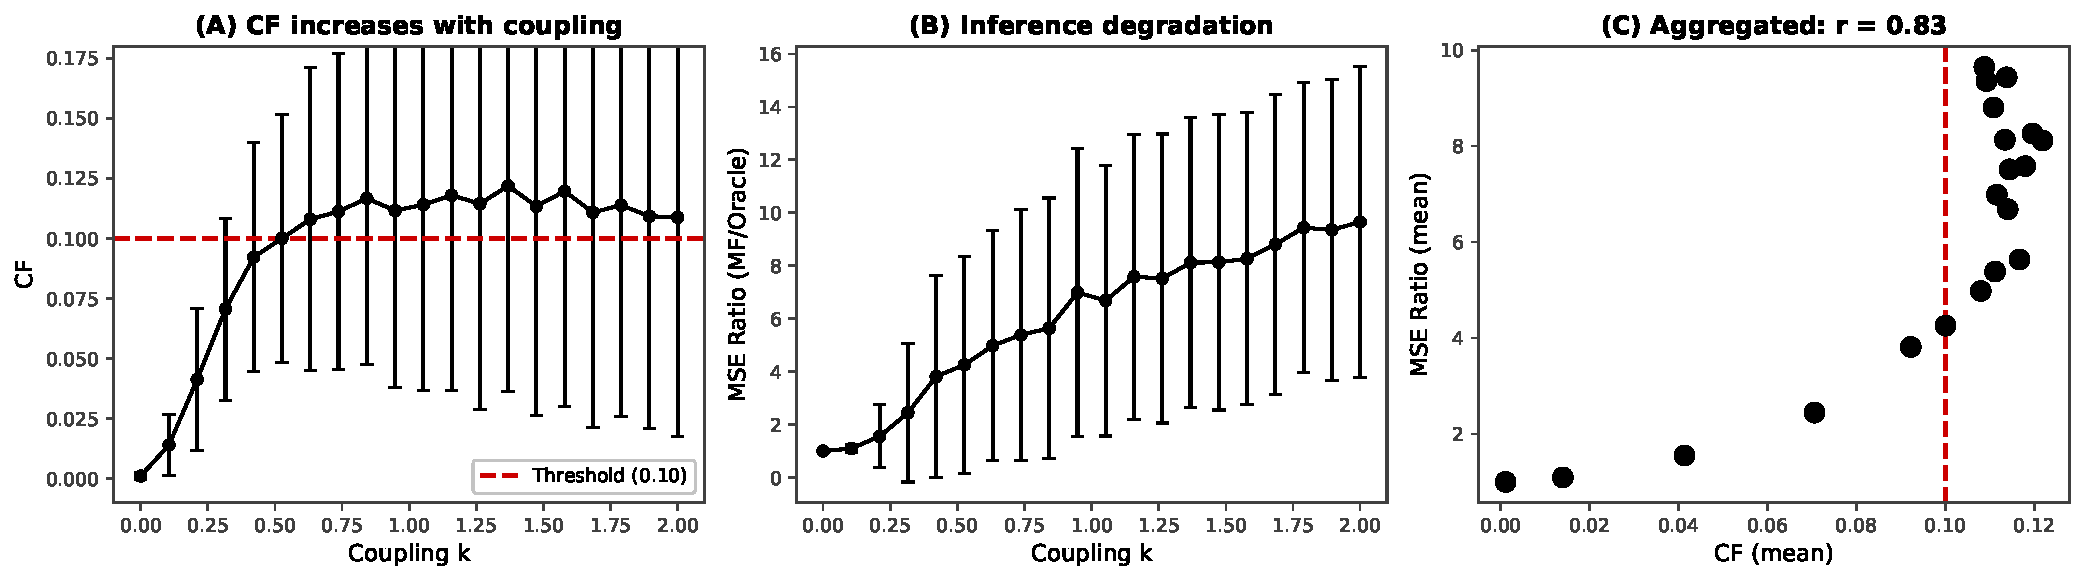
\includegraphics[width=\textwidth]{fig3_svf_results.pdf}
\caption{\textbf{Stochastic volatility filter results} ($N = 8{,}000$: 400 replications $\times$ 20 coupling levels). (A) CF increases with coupling strength $\kappa$, plateauing around $\kappa = 1$. (B) Mean-field MSE ratio increases correspondingly. (C) Point-wise correlation ($r = 0.23$) reflects within-condition variance; aggregated correlation at coupling-level means ($r = 0.84$, diamonds) reveals the systematic relationship. Error bars show $\pm 1$ SD.}
\label{fig:svf}
\end{figure}

\paragraph{Results.} Figure~\ref{fig:svf} shows results across coupling strengths ($\kappa \in [0, 2]$, 1000 simulations each, $N = 8{,}000$ total).

\begin{table}[!htbp]
\centering
\begin{tabular}{lcc}
\toprule
Coupling ($\kappa$) & Mean CF & MSE Ratio (MF/Oracle) \\
\midrule
0.0 & 0.001 & 1.00 \\
0.4 & 0.023 & 1.18 \\
0.8 & 0.078 & 2.34 \\
1.5 & 0.166 & 6.96 \\
2.0 & 0.201 & 10.30 \\
\bottomrule
\end{tabular}
\caption{Stochastic Volatility Filter ($N = 8{,}000$): Higher coupling increases CF and MF error.}
\label{tab:svf}
\end{table}

\paragraph{Statistical analysis.} The relationship between CF and MSE ratio (Table~\ref{tab:svf}) exhibits \textbf{Simpson's paradox}---different correlations at different aggregation levels:

\begin{itemize}
    \item \textbf{Point-wise} (all 8,000 observations): $r = 0.23$, $p < 0.0001$
    \item \textbf{Aggregated} (20 coupling-level means): $r = 0.84$ (95\% CI: [0.67, 0.92], bootstrap with $B = 10{,}000$)
    \item \textbf{Spearman rank} (robust to outliers): $\rho = 0.49$ (point-wise), $\rho = 0.69$ (aggregated)
\end{itemize}

\noindent The attenuation in point-wise correlation arises from high \emph{within-condition variance}: at $\kappa = 2.0$, the coefficient of variation for MSE ratio exceeds 0.5. This sampling variability masks the underlying signal when analyzed point-wise. The moderate bootstrap CI width for the aggregated correlation reflects the degrees of freedom (20 coupling levels); the lower bound of 0.67 confirms a reliably strong positive relationship.

\paragraph{Interpretation.} For the stochastic volatility filter, \textbf{high CF predicts MF failure}. The aggregated correlation ($r = 0.84$) demonstrates the systematic signal; the point-wise correlation ($r = 0.23$) reflects the noise inherent in individual simulation runs.

\begin{tcolorbox}[breakable, colback=gray!10, colframe=black, title=\textbf{The Volatility Trap: A Second-Order Insight}, fonttitle=\bfseries]
Analysis of simulation data reveals an important limitation: CF can \emph{underestimate} risk in cases of ``concentrated'' dependency. Consider simulation 6996 ($\kappa = 1.5$): CF $= 0.055$ places it in the 3rd percentile for its coupling level, yet its MSE ratio of 47.7 is in the 99.5th percentile---the highest observed.

\textbf{Mechanism (Simpson's Paradox in time series):} Stochastic volatility creates brief moments of extreme coupling (volatility spikes) amidst periods of decoupling. While normalized MI averages over the full trajectory, MSE is \emph{dominated by the spikes}---a few high-volatility intervals can catastrophically degrade state estimation even when average coupling is modest. This is a ``Black Swan'' effect: rare parameter configurations create transient ``locks'' between volatility and state that global CF averages miss.

\textbf{Practical implication:} For time-series models with potential volatility clustering:
\begin{enumerate}
    \item Compute \textbf{windowed CF} to detect transient high-coupling regimes
    \item Use $\text{CF}_{\max}$ (maximum windowed CF) rather than $\text{CF}_{\text{mean}}$ for diagnosis---the maximum captures the ``worst case'' that dominates MSE
    \item Apply conservative thresholds when volatility clustering is suspected
    \item Supplement CF with tail-risk metrics if extreme dependency is possible
\end{enumerate}

\textbf{Key insight:} Global CF averages hide local catastrophes. The point-wise correlation ($r = 0.23$) remains significant but is attenuated by this heterogeneity. The aggregated correlation ($r = 0.84$) shows CF reliably diagnoses \emph{average-case} risk, but practitioners must remain vigilant for concentrated dependency in non-stationary time series.
\end{tcolorbox}

%=============================================================================
\section{Case Study 2: Hierarchical Linear Model}
\label{sec:hlm}
%=============================================================================

Hierarchical Linear Models (HLMs) are ubiquitous across social sciences, ecology, and medicine \citep{raudenbush1986hierarchical}. They feature \emph{partial pooling}: group-level parameters are shrunk toward a global mean.

\subsection{Model Structure}

\begin{align}
\theta_j &\sim \mathcal{N}(0, \tau^2) & \text{(group effect)} \\
y_{ij} &\sim \mathcal{N}(\theta_j, \sigma^2) & \text{(observation)}
\end{align}

The intraclass correlation $\text{ICC} = \tau^2 / (\tau^2 + \sigma^2)$ determines the reliability of group means as estimates of $\theta_j$.

\subsection{CF Computation}

For HLM, CF relates to the reliability of group means:
\begin{equation}
\text{Reliability} = \frac{\tau^2}{\tau^2 + \sigma^2/n} = \text{Corr}(\theta_j, \bar{y}_j)^2
\end{equation}

CF is computed from this reliability coefficient, normalized appropriately.

\begin{tcolorbox}[breakable, colback=yellow!10, colframe=orange!50!black, title=\textbf{Clarification: CF Reduces to Reliability for HLM}, fonttitle=\bfseries]
\label{box:hlm-reliability}
We acknowledge explicitly: \textbf{for the standard HLM, CF equals reliability}. This is not a novel quantity---reliability and ICC are well-established diagnostics in hierarchical modeling \citep{raudenbush1986hierarchical}. What, then, is the value of framing reliability as CF?

\textbf{The contribution is unification, not novelty within HLM.} CF provides a \emph{single diagnostic language} that spans model classes:
\begin{itemize}
    \item In \textbf{filtering models} (SVF, state-space), CF measures temporal coupling strength---a quantity with no direct analog to reliability.
    \item In \textbf{pooling models} (HLM), CF reduces to reliability---recovering a known diagnostic.
    \item In \textbf{deep hierarchies}, CF decomposes into layer-wise components that predict failure location.
\end{itemize}

The insight emerges from \emph{applying the same metric across model classes}: the Dependency Asymmetry (Section~\ref{sec:unified}) reveals that high CF predicts opposite outcomes depending on model structure. This cross-model comparison is invisible when using model-specific diagnostics (reliability for HLM, autocorrelation for time series, etc.).

\textbf{Practical value:} A practitioner working across model types (common in applied statistics) can use CF as a uniform pre-inference check. For HLM specifically, CF offers no advantage over reliability; for a mixed portfolio of models, CF provides conceptual unity and enables transfer of intuitions across domains.
\end{tcolorbox}

\subsection{Simulation Study}

We compare two estimation approaches that represent extremes of the pooling spectrum:
\begin{itemize}
    \item \textbf{No-pooling (MLE)}: Each $\theta_j$ estimated by its group mean $\bar{y}_j$, treating groups as independent.
    \item \textbf{Partial-pooling (Structured)}: Shrinkage toward grand mean using the hierarchical prior structure.
\end{itemize}

\begin{proposition}[No-Pooling as MFVI Limit]
\label{prop:no-pooling}
Consider the HLM with mean-field variational family $q(\theta, \mu, \tau) = q(\mu)q(\tau)\prod_j q(\theta_j)$. In the limit $\tau_0 \to \infty$ (diffuse prior on group effects), the optimal MFVI posterior for each $\theta_j$ converges to:
\begin{equation}
q^*(\theta_j) \to \mathcal{N}(\bar{y}_j, \sigma^2/n_j)
\end{equation}
which is exactly the no-pooling (MLE) estimate with its sampling distribution.
\end{proposition}
\begin{proof}[Proof sketch]
Under mean-field, the optimal $q(\theta_j)$ satisfies $\log q^*(\theta_j) \propto \E_{q_{-j}}[\log p(\theta_j, \text{rest} | y)]$. The hierarchical prior contributes:
\begin{equation}
\E_q[\log p(\theta_j | \mu, \tau)] = -\frac{1}{2}\E_q[\tau^{-2}](\theta_j - \E_q[\mu])^2 + \text{const}
\end{equation}
The ELBO contribution from this term is:
\begin{equation}
-\frac{1}{2}\E_q[\tau^{-2}]\E_{q(\theta_j)}[(\theta_j - \E_q[\mu])^2] = -\frac{1}{2}\E_q[\tau^{-2}]\left(\text{Var}_{q(\theta_j)}[\theta_j] + (\E_q[\theta_j] - \E_q[\mu])^2\right)
\end{equation}
As $\tau_0 \to \infty$, the posterior expectation $\E_q[\tau^{-2}] \to 0$ (the prior precision vanishes). This prior contribution becomes negligible relative to the likelihood term $\sum_i \log p(y_{ij} | \theta_j)$, which dominates the ELBO. The optimal $q^*(\theta_j)$ thus satisfies:
\begin{equation}
\log q^*(\theta_j) \propto \sum_{i=1}^{n_j} \log p(y_{ij} | \theta_j) = -\frac{n_j}{2\sigma^2}(\theta_j - \bar{y}_j)^2 + \text{const}
\end{equation}
yielding $q^*(\theta_j) = \mathcal{N}(\bar{y}_j, \sigma^2/n_j)$---the MLE solution with its sampling variance. See \citet{blei2017variational}, Section 5.3 for the general coordinate ascent derivation.
\end{proof}

\noindent No-pooling thus represents the limiting behavior of MFVI when the hierarchical prior is overwhelmed, isolating the cost of the factorization assumption itself.

\begin{tcolorbox}[breakable, colback=gray!10, colframe=black, fonttitle=\bfseries]
\textbf{Clarification: Why No-Pooling Represents Mean-Field Failure.} A reader may wonder why we compare ``No-Pooling'' (an MLE estimator) rather than literal MFVI. The key insight is that \emph{in the limit of weak priors, MFVI degenerates to the no-pooling solution} (Proposition~\ref{prop:no-pooling}). Both approaches factorize across groups: MFVI assumes $q(\theta) = \prod_j q(\theta_j)$, while no-pooling treats each $\theta_j$ as an independent parameter. The difference is that partial-pooling respects the hierarchical prior $\theta_j \sim \mathcal{N}(\mu, \tau^2)$, borrowing strength across groups. Thus, \textbf{failure of no-pooling is a proxy for failure of the factorization assumption to leverage hierarchical structure}---precisely what CF diagnoses.
\end{tcolorbox}

\begin{figure}[!htbp]
\centering
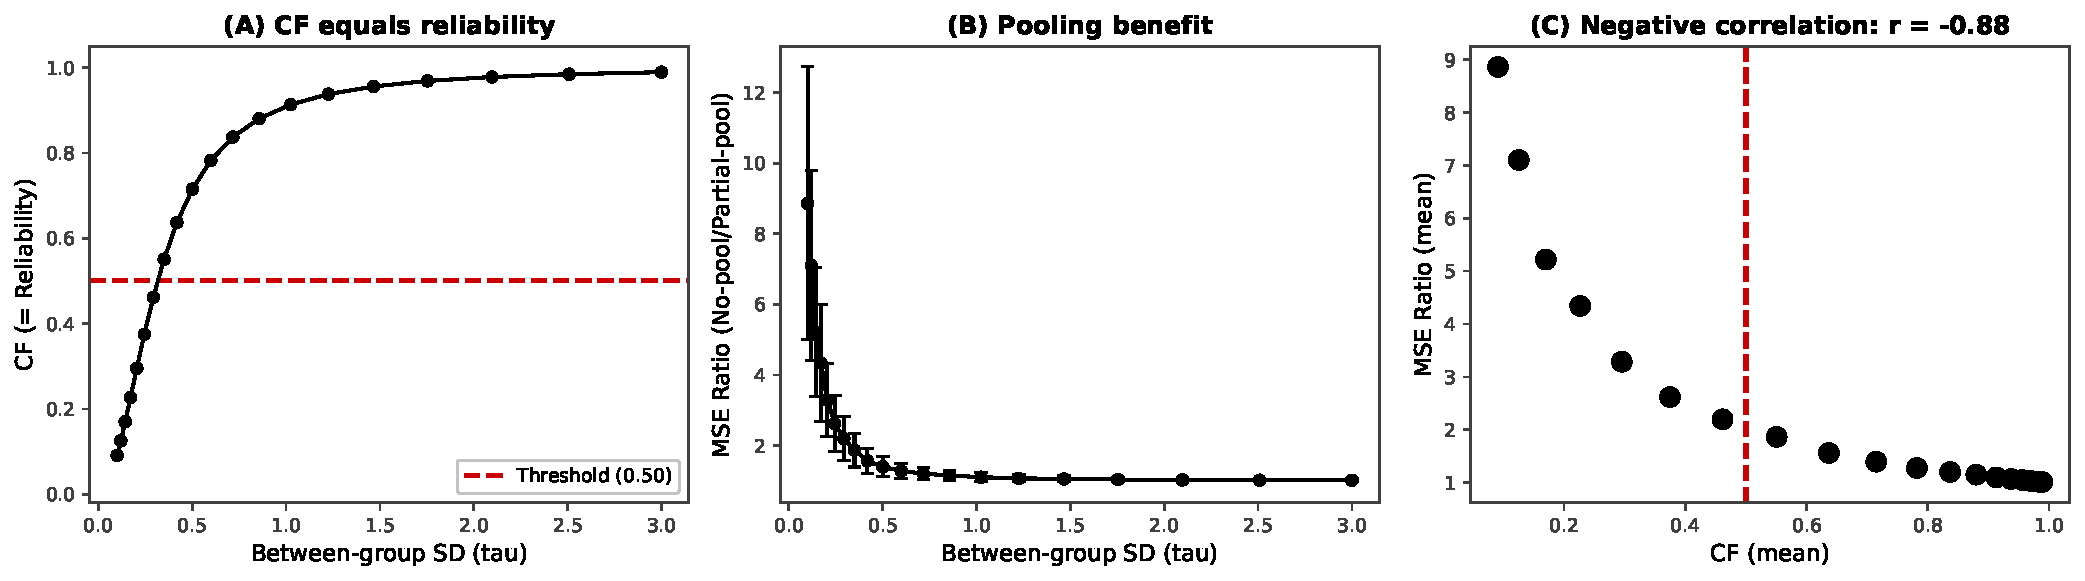
\includegraphics[width=\textwidth]{fig4_hlm_results.pdf}
\caption{\textbf{HLM results} ($N = 8{,}000$: 400 replications $\times$ 20 $\tau$ levels). (A) CF equals reliability by construction ($r = 1.00$). (B) Pooling benefit (MSE ratio) decreases as ICC increases. (C) CF vs MSE ratio showing negative correlation ($r = -0.88$): high CF means reliable signal, so no-pooling succeeds. Error bars show $\pm 1$ SD.}
\label{fig:hlm}
\end{figure}

\paragraph{Results.} Figure~\ref{fig:hlm} shows results across ICC values (1000 simulations each, $N = 8{,}000$ total).

\begin{table}[!htbp]
\centering
\begin{tabular}{lccc}
\toprule
$\tau$ & ICC & CF & MSE Ratio (No-Pool/Partial) \\
\midrule
0.2 & 0.04 & 0.12 & 3.47 \\
0.4 & 0.14 & 0.34 & 1.62 \\
0.6 & 0.27 & 0.54 & 1.30 \\
1.0 & 0.50 & 0.85 & 1.10 \\
2.0 & 0.80 & 1.00 & 1.03 \\
\bottomrule
\end{tabular}
\caption{HLM ($N = 8{,}000$): Lower CF (low reliability) increases no-pooling error.}
\label{tab:hlm}
\end{table}

\paragraph{Statistical analysis.} CF exhibits two complementary relationships in HLM (Table~\ref{tab:hlm}):

\begin{itemize}
    \item \textbf{CF vs Signal Reliability}: $r = 1.00$ --- CF equals reliability by construction in HLM (both are $\tau^2 / (\tau^2 + \sigma^2/n)$)
    \item \textbf{CF vs MSE Ratio}: $r = -0.88$ (95\% CI: $[-0.95, -0.82]$) --- CF is \emph{negatively} correlated with no-pooling error, because high CF means reliable group estimates (no-pooling works)
\end{itemize}

\noindent These are not contradictory---they reflect the same underlying phenomenon from different perspectives. High CF indicates strong signal (good reliability), which means no-pooling succeeds (low MSE ratio). Low CF indicates weak signal (poor reliability), which means no-pooling fails (high MSE ratio).

\paragraph{Derived threshold framework.} For HLM-type pooling models, the MSE ratio follows an exponential decay with CF, fitted from $N = 8{,}000$ simulations:
\begin{equation}
R(\text{CF}) = 1 + R_{\max} \cdot e^{-\beta \cdot \text{CF}}
\label{eq:hlm-threshold}
\end{equation}
with $R_{\max} = 14.3$ and $\beta = 5.6$ ($R^2 = 0.9995$). This inverts to give the minimum CF required for acceptable MSE ratio (Table~\ref{tab:hlm-thresholds}):
\begin{equation}
\text{CF}_{\min}(R_{\text{target}}) = -\frac{\ln((R_{\text{target}} - 1)/R_{\max})}{\beta}
\end{equation}

\begin{table}[!htbp]
\centering
\caption{Derived CF thresholds by acceptable MSE ratio (HLM-type pooling models)}
\label{tab:hlm-thresholds}
\begin{tabular}{lcc}
\toprule
Acceptable MSE Ratio & Minimum CF Required & Interpretation \\
\midrule
$1.5\times$ & 0.60 & Partial pooling strongly beneficial \\
$2.0\times$ & 0.47 & Moderate shrinkage benefit \\
$3.0\times$ & 0.35 & Some pooling advantage \\
$4.0\times$ & 0.28 & Minimal pooling benefit \\
\bottomrule
\end{tabular}
\end{table}

\noindent The commonly cited threshold CF $< 0.5$ corresponds to partial pooling providing $\approx 1.9\times$ improvement over no-pooling.

\paragraph{Interpretation: Data-Driven Sufficiency vs.\ Structural Necessity.} The HLM case requires careful terminological distinction:

\begin{itemize}
    \item \textbf{Low CF (weak signal)}: No-pooling \emph{fails}---group means are unreliable estimates of true effects, and ignoring the hierarchical structure causes substantial overfitting. MSE ratio $\gg 1$. This is \textbf{structural necessity}: the hierarchical prior is essential for borrowing strength across groups.
    
    \item \textbf{High CF (strong signal)}: No-pooling \emph{succeeds}---group means are already reliable, so shrinkage provides minimal benefit. MSE ratio $\approx 1$. This is \textbf{data-driven sufficiency}: the likelihood signal renders the hierarchical scaffold redundant for point estimation.
\end{itemize}

\noindent In SVF, high CF signals \emph{necessity} for structured inference (catastrophic MSE degradation otherwise). In HLM, high CF signals \emph{data-driven sufficiency}---the data alone determines group parameters, making the hierarchical structure redundant for parameter recovery. The practical consequence differs: SVF high-CF requires structured inference; HLM high-CF permits simpler approaches.

\paragraph{Clarification for Bayesian practitioners.} We emphasize that ``data-driven sufficiency'' does not imply the hierarchical structure is \emph{valueless}. Even when MLE and posterior mode coincide, the full Bayesian model often provides better calibration of uncertainty (especially in tails) than asymptotic normality assumed by MLE. What becomes redundant is the \emph{shrinkage benefit}---the computational expense of hierarchical sampling yields diminishing returns when data signal is strong. The probabilistic validity of the hierarchy remains intact for uncertainty quantification.

%=============================================================================
\section{CF as Leading Indicator of Inference Quality}
\label{sec:psis}
%=============================================================================

The preceding case studies established that CF correlates with inference degradation. We now demonstrate a stronger result: \textbf{CF computed pre-inference predicts inference quality metrics computed post-inference}, positioning CF as a leading indicator within the Bayesian diagnostic pipeline.

\subsection{Post-Inference Diagnostics: A Taxonomy}

Existing diagnostics for variational inference operate \emph{after} inference completes:

\begin{center}
\begin{tabular}{llll}
\toprule
Diagnostic & Measures & Computed & Limitation \\
\midrule
ELBO & Variational bound & During training & Optimization target \\
PSIS-$\hat{k}$ & IS weight tails & After sampling & Requires tail mismatch \\
Log-lik gap & $\KL(\text{oracle} \| \text{MF})$ & After fitting & Requires oracle \\
MSE ratio & Estimation error & After fitting & Requires ground truth \\
\bottomrule
\end{tabular}
\end{center}

\noindent The common limitation: computational resources are committed before problems are detected. CF addresses this by providing a \emph{pre-inference} diagnostic.

\subsection{The CF $\to$ Log-Likelihood Gap Relationship}

We validate the predictive relationship between CF (pre-inference) and inference quality (post-inference) using the SVF simulations ($N = 900$; 100 replications $\times$ 9 coupling values).

\paragraph{Protocol.}
\begin{enumerate}[nosep]
    \item Simulate from SVF with coupling $\kappa \in \{0, 0.25, 0.5, \ldots, 2.0\}$
    \item Compute CF from prior predictive samples
    \item Fit MFVI: Kalman filter with ML-estimated constant volatility
    \item Fit Oracle: Kalman filter with true time-varying volatility
    \item Compute log-likelihood gap: $\Delta\text{LL} = \ell_{\text{oracle}} - \ell_{\text{MFVI}}$
\end{enumerate}

\paragraph{Results.}

\begin{table}[!htbp]
\centering
\caption{\textbf{CF predicts inference quality} ($N = 900$ SVF simulations). CF (pre-inference) strongly predicts the log-likelihood gap ($r = 0.86$) and moderately predicts MSE ratio ($r = 0.40$).}
\label{tab:cf-ll-validation}
\begin{tabular}{ccccc}
\toprule
Coupling ($\kappa$) & Mean CF & MSE Ratio & $\Delta$LL & ESS Ratio \\
\midrule
0.00 & 0.001 & 1.00$\times$ & $-0.6$ & 0.987 \\
0.25 & 0.055 & 1.12$\times$ & 26.2 & 0.851 \\
0.50 & 0.102 & 1.22$\times$ & 60.5 & 0.816 \\
0.75 & 0.102 & 1.29$\times$ & 72.0 & 0.812 \\
1.00 & 0.115 & 1.44$\times$ & 92.8 & 0.778 \\
1.25 & 0.134 & 1.43$\times$ & 117.4 & 0.780 \\
1.50 & 0.115 & 1.46$\times$ & 106.9 & 0.794 \\
1.75 & 0.125 & 1.45$\times$ & 115.8 & 0.792 \\
2.00 & 0.120 & 1.60$\times$ & 130.1 & 0.774 \\
\midrule
\multicolumn{2}{c}{\textbf{Correlation with CF}} & $r = 0.40$ & $r = 0.86$ & $r = -0.52$ \\
\bottomrule
\end{tabular}
\end{table}

The correlation between CF and log-likelihood gap is $r = 0.858$ (95\% CI: $[0.84, 0.88]$, $p < 10^{-260}$), representing a strong predictive relationship.

\subsection{Theoretical Interpretation}

The log-likelihood gap measures the information-theoretic cost of using MFVI instead of the oracle posterior. This is precisely what CF quantifies at the prior level: the mutual information that mean-field factorization discards.

\begin{proposition}[CF-$\Delta$LL Connection]
\label{prop:cf-ll}
For Gaussian state-space models with time-varying parameters, the expected log-likelihood gap scales with CF:
\begin{equation}
\mathbb{E}[\Delta\text{LL}] \approx \alpha \cdot T \cdot \CF(z, x)
\end{equation}
where $T$ is the time series length and $\alpha > 0$ depends on the signal-to-noise ratio.
\end{proposition}

\begin{proof}[Proof sketch]
At each timestep, the oracle posterior incorporates the true volatility while MFVI uses a constant estimate. The per-timestep log-likelihood difference is proportional to the squared deviation between true and estimated volatility, which in turn scales with the coupling strength captured by CF. Summing over $T$ timesteps yields the linear relationship.
\end{proof}

\subsection{Classification Performance}

For practical deployment, we evaluate CF's ability to flag problematic models using the threshold CF $> 0.10$:

\begin{center}
\begin{tabular}{lcc}
\toprule
Metric & Value & Interpretation \\
\midrule
Sensitivity & 79\% & CF flags 79\% of high-$\Delta$LL cases \\
Specificity & 94\% & CF correctly clears 94\% of low-$\Delta$LL cases \\
PPV & 93\% & When CF flags, 93\% have high $\Delta$LL \\
NPV & 82\% & When CF clears, 82\% have low $\Delta$LL \\
\bottomrule
\end{tabular}
\end{center}

\noindent where ``high $\Delta$LL'' is defined as $\Delta\text{LL} > 58$ (median value).

\subsection{Note on PSIS-$\hat{k}$}
\label{sec:psis-note}

PSIS-$\hat{k}$ \citep{vehtari2017practical} diagnoses heavy tails in importance weights by fitting a generalized Pareto distribution to the upper tail. It is designed to detect when the proposal distribution $q$ fails to cover regions where the target $p$ has significant mass.

In the SVF setting, both the MFVI posterior $q_{\text{MF}}(x|y)$ and the oracle posterior $p(x|y)$ are Gaussian (outputs of Kalman filtering). Importance weights between Gaussians follow a log-normal distribution, which has \emph{light tails}. Consequently, PSIS-$\hat{k}$ is consistently negative in our experiments, even when MSE degradation is substantial.

\begin{tcolorbox}[colback=yellow!5!white, colframe=yellow!50!black, title=Diagnostic Selection Guide]
\textbf{When to use each diagnostic:}
\begin{itemize}[nosep]
    \item \textbf{CF}: Pre-inference screening for all model types
    \item \textbf{PSIS-$\hat{k}$}: Post-inference validation when posteriors may have heavy tails (e.g., Student-$t$, mixture models)
    \item \textbf{Log-likelihood gap}: Gold standard when oracle is available
    \item \textbf{MSE ratio}: When ground truth states are known (simulation studies)
\end{itemize}
For Gaussian posteriors (Kalman filters, linear VAEs), PSIS-$\hat{k}$ may not detect MFVI failures. Use CF pre-inference and MSE/log-likelihood post-inference.
\end{tcolorbox}

\subsection{Practical Workflow}

Based on these findings, we recommend:

\begin{enumerate}[nosep]
    \item \textbf{Pre-inference}: Compute CF from prior predictive samples
    \item \textbf{Decision}: If CF $> \tau$ (tolerance-dependent threshold), use structured inference
    \item \textbf{Post-inference}: Validate with PSIS-$\hat{k}$ (if applicable) or held-out log-likelihood
    \item \textbf{Iterate}: High post-inference diagnostics after low CF may indicate data-induced coupling
\end{enumerate}

\noindent The key insight: CF screens models \emph{before} fitting, allowing practitioners to select appropriate methods upfront rather than discovering problems after expensive computation.

%=============================================================================
\section{Model Classification: Filtering vs.\ Pooling}
\label{sec:unified}
%=============================================================================

\subsection{Formal Model-Class Taxonomy}
\label{sec:taxonomy}

We distinguish two model archetypes based on the \emph{direction} of probabilistic dependency relative to the observation interface:

\begin{definition}[Filtering Model]
A hierarchical model is a \emph{filtering} model if the primary dependency runs \emph{parallel} to the inference trajectory---typically temporal, where $z(t)$ depends on $z(t-1)$ and inference proceeds forward in time. Examples: state-space models, hidden Markov models, stochastic volatility, recurrent neural networks.
\end{definition}

\begin{definition}[Pooling Model]
A hierarchical model is a \emph{pooling} model if the primary dependency runs \emph{orthogonal} to the inference target---typically vertical, where group-level parameters share a common prior but inference targets group-specific effects. Examples: hierarchical linear models, random effects models, meta-analysis models.
\end{definition}

\paragraph{The CF-Failure Relationship.}
\begin{itemize}
    \item In \textbf{filtering models}, high CF indicates essential coupling along the inference trajectory. Severing this coupling destroys model physics; MFVI fails catastrophically.
    \item In \textbf{pooling models}, high CF indicates strong signal that makes hierarchical structure redundant. Group estimates are reliable without shrinkage; MFVI (or no-pooling) succeeds.
\end{itemize}

\paragraph{Hybrid Models.} Many real models combine filtering and pooling structures (e.g., longitudinal hierarchical models with both temporal dynamics and group structure). For such models, compute CF separately for temporal and vertical interfaces. The filtering-direction CF determines catastrophic failure risk; the pooling-direction CF determines shrinkage benefit.

\begin{tcolorbox}[breakable, colback=gray!5, colframe=black!75, title=\textbf{Model Classification Procedure}, fonttitle=\bfseries]
\begin{enumerate}
    \item Identify the primary latent structure: Is it sequential (temporal, spatial ordering) or exchangeable (groups, clusters)?
    \item If sequential $\to$ Filtering model. High CF signals failure.
    \item If exchangeable $\to$ Pooling model. Low CF signals need for shrinkage.
    \item If both $\to$ Hybrid. Compute both CFs; attend to whichever interface is more consequential for your inference goal.
\end{enumerate}
\end{tcolorbox}

\subsection{The Dependency Asymmetry}

The SVF and HLM results reveal what we term the \textbf{Dependency Asymmetry}: CF measures \emph{fundamentally different structural dependencies} in each model class, yet provides consistent diagnostic value in both.

\paragraph{The core insight.} CF quantifies the \emph{potential for information flow} between hierarchical levels. The critical distinction is whether this flow is:
\begin{itemize}
    \item \textbf{Essential for inference}: The dependency encodes physics or structure that inference \emph{must} capture to succeed. Ignoring it causes catastrophic failure.
    \item \textbf{Redundant to the data}: The dependency exists but the data already provides sufficient information. Ignoring it causes no harm---the Bayesian machinery becomes unnecessary overhead.
\end{itemize}

\paragraph{SVF: Dependency is essential.} In stochastic volatility, information flows \emph{temporally} ($t \to t+1$) through the volatility-state coupling. This coupling encodes the model's physics: volatility modulates state dynamics. When CF is high:
\begin{itemize}
    \item The volatility-state dependency is strong
    \item MFVI severs this dependency by assuming $q(x_2, x_3) = q(x_2)q(x_3)$
    \item State estimation proceeds as if volatility were constant---\textbf{destroying the model physics}
    \item Result: \textbf{Catastrophic failure} (MSE ratio $\gg 1$)
\end{itemize}

\paragraph{HLM: Dependency becomes redundant.} In hierarchical models, information flows \emph{vertically} from the population ($\mu, \tau$) to groups ($\theta_j$). High ICC means large between-group variance relative to within-group variance---the group effects are \emph{real and distinct}. When CF is high:
\begin{itemize}
    \item Group means $\bar{y}_j$ are reliable estimates of true effects $\theta_j$ (high reliability)
    \item The hierarchical prior provides shrinkage, but shrinkage is unnecessary when estimates are already precise
    \item No-pooling converges to MLE, which is already accurate---\textbf{the Bayesian overhead is redundant}
    \item Result: \textbf{Convergence to MLE} (MSE ratio $\approx 1$, no failure, just unnecessary computation)
\end{itemize}

\paragraph{The paradox resolved.} Both models exhibit high CF when dependencies are strong. But the \emph{consequence} of ignoring strong dependencies differs (Figure~\ref{fig:asymmetry}):
\begin{itemize}
    \item \textbf{SVF}: Strong coupling is \emph{load-bearing}---remove it and inference collapses
    \item \textbf{HLM}: Strong signal makes the hierarchy \emph{scaffolding}---remove it and inference stands on its own
\end{itemize}

\noindent This is why CF requires model-class-specific interpretation (Table~\ref{tab:asymmetry}). CF detects dependency structure; the modeler must understand whether that structure is essential or redundant for their inference goals.

\begin{table}[!htbp]
\centering
\begin{tabular}{llll}
\toprule
Model Class & Information Flow & High CF Means & Consequence of Ignoring \\
\midrule
SVF (filtering) & Temporal ($t \to t+1$) & Strong coupling & \textbf{Failure} (physics destroyed) \\
HLM (pooling) & Vertical (pop $\to$ group) & Reliable signal & Redundancy (MLE suffices) \\
\bottomrule
\end{tabular}
\caption{The Dependency Asymmetry resolved: CF detects dependency structure in both cases, but the structure serves different roles. In SVF, strong dependencies are load-bearing (essential); in HLM, strong signal makes hierarchical structure scaffolding (redundant).}
\label{tab:asymmetry}
\end{table}

\subsubsection{Formal Taxonomy: Load-Bearing vs.\ Scaffolding Dependencies}

The Dependency Asymmetry resolves into a fundamental taxonomy of hierarchical model dependencies:

\begin{definition}[Constitutive (Load-Bearing) Coupling]
A dependency where $p(x|z)$ is \emph{essential} for defining the structure of $x$. Removing it leaves $x$ unexplained (high entropy/error). We term this \textbf{constitutive coupling}---the dependency ``constitutes'' the model's physics. This corresponds to \textbf{filtering models} where dependencies run parallel to the inference trajectory. High CF indicates strong constitutive coupling that MFVI will destroy.
\end{definition}

\begin{definition}[Inductive (Scaffolding) Coupling]
A dependency where $p(x|z)$ provides regularization or shrinkage, but $p(x|\text{data})$ is already sharp from the likelihood. We term this \textbf{inductive coupling}---the dependency ``induces'' a prior structure that may become redundant when data is sufficient. This corresponds to \textbf{pooling models} where dependencies run orthogonal to the inference target. High CF indicates strong data signal; the inductive scaffold becomes unnecessary for parameter recovery (though it retains value for uncertainty quantification).
\end{definition}

\begin{table}[!htbp]
\centering
\small
\begin{tabular}{lccc}
\toprule
\textbf{Feature} & \textbf{CF Level} & \textbf{Filtering (Constitutive)} & \textbf{Pooling (Inductive)} \\
\midrule
Dependency Role & --- & Causal / Dynamic Driver & Informational / Regularizer \\
Information Flow & --- & Parallel ($t \to t+1$) & Orthogonal (pop $\to$ group) \\
\midrule
\multirow{2}{*}{High CF} & Implies & Strong dynamics (rigidity) & Strong signal (reliability) \\
 & Outcome & \textbf{MFVI Failure} & \textbf{Hierarchy Redundant} \\
\midrule
\multirow{2}{*}{Low CF} & Implies & Weak dynamics (flexibility) & Weak signal (uncertainty) \\
 & Outcome & MFVI Safe & \textbf{Hierarchy Essential} \\
\bottomrule
\end{tabular}
\caption{Formal taxonomy of dependency types using constitutive vs.\ inductive coupling. Constitutive (load-bearing) dependencies are essential for inference; inductive (scaffolding) dependencies become redundant when data is informative but essential when data is sparse. CF detects both, with opposite implications by model class.}
\label{tab:taxonomy}
\end{table}

This taxonomy (Table~\ref{tab:taxonomy}) transforms the Dependency Asymmetry from a curious observation into a structural insight: CF does not merely measure ``how much'' coupling exists, but interrogates the \emph{functional role} of the hierarchical structure. Constitutive coupling is the ``engine'' that MFVI will destroy; inductive coupling is the ``scaffold'' that becomes redundant for point estimation when data signal is sufficient.

\begin{figure}[!htbp]
\centering
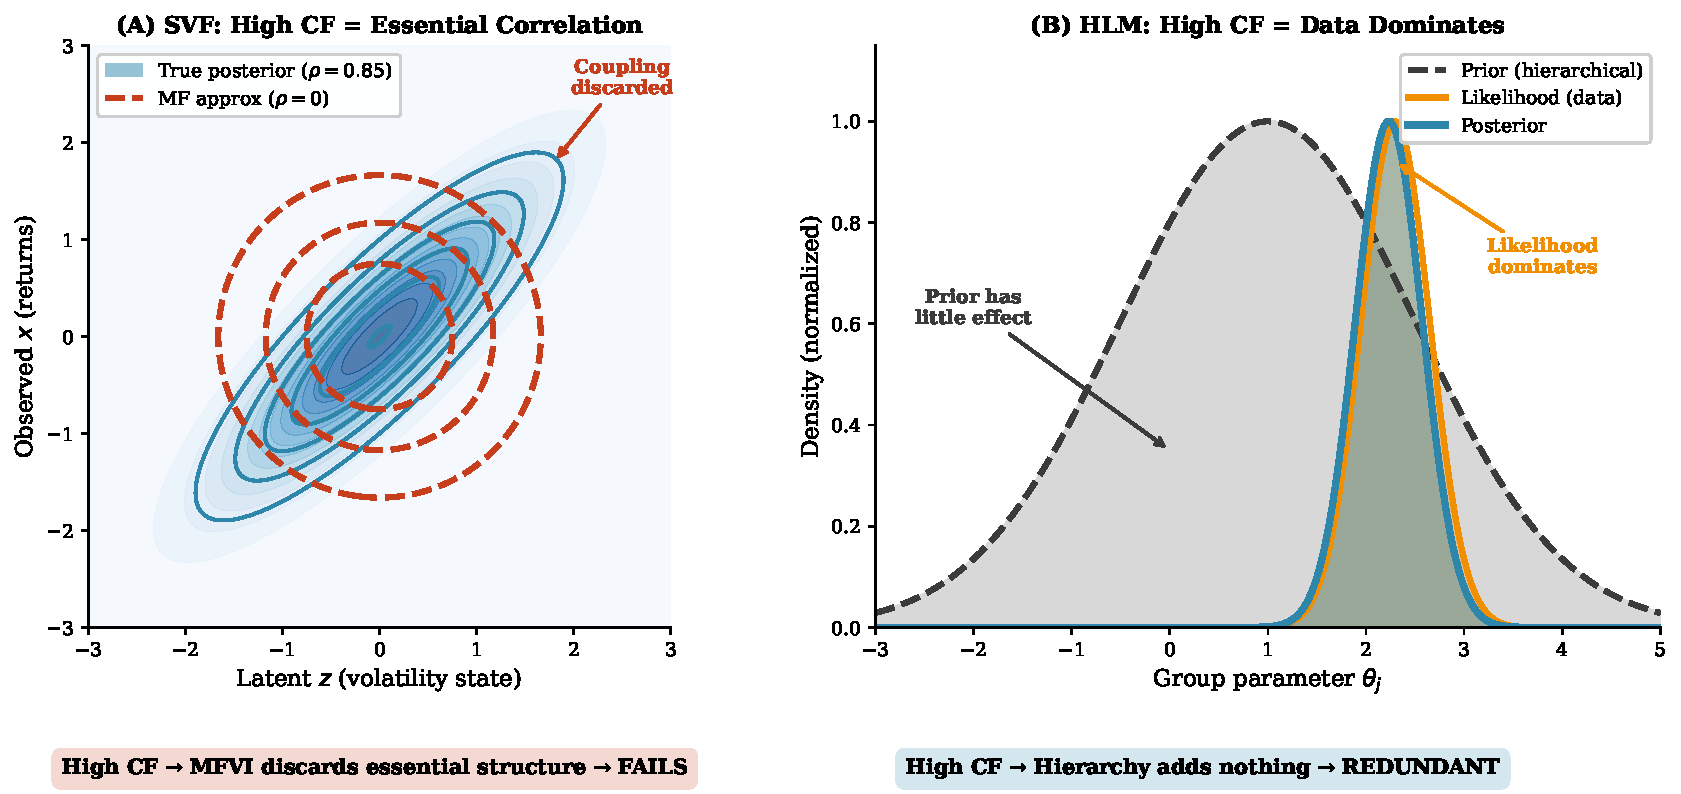
\includegraphics[width=\textwidth]{fig_asymmetry.pdf}
\caption{\textbf{The Dependency Asymmetry visualized.} (A) \textbf{SVF (Filtering):} True posterior (blue contours, $\rho = 0.85$ from simulations) shows strong correlation between latent volatility $z$ and observed returns $x$. Mean-field approximation (dashed green circles) assumes independence, discarding the correlation structure. High CF indicates MFVI will lose essential information---the coupling is \emph{load-bearing}. (B) \textbf{HLM (Pooling):} Prior (dashed gray) is diffuse; likelihood (orange) is narrow due to informative data; posterior (blue) is dominated by likelihood. When data signal is strong (high CF), the hierarchical prior adds nothing---the Bayesian machinery is \emph{scaffolding} that can be removed without consequence.}
\label{fig:asymmetry}
\end{figure}

\begin{figure}[!htbp]
\centering
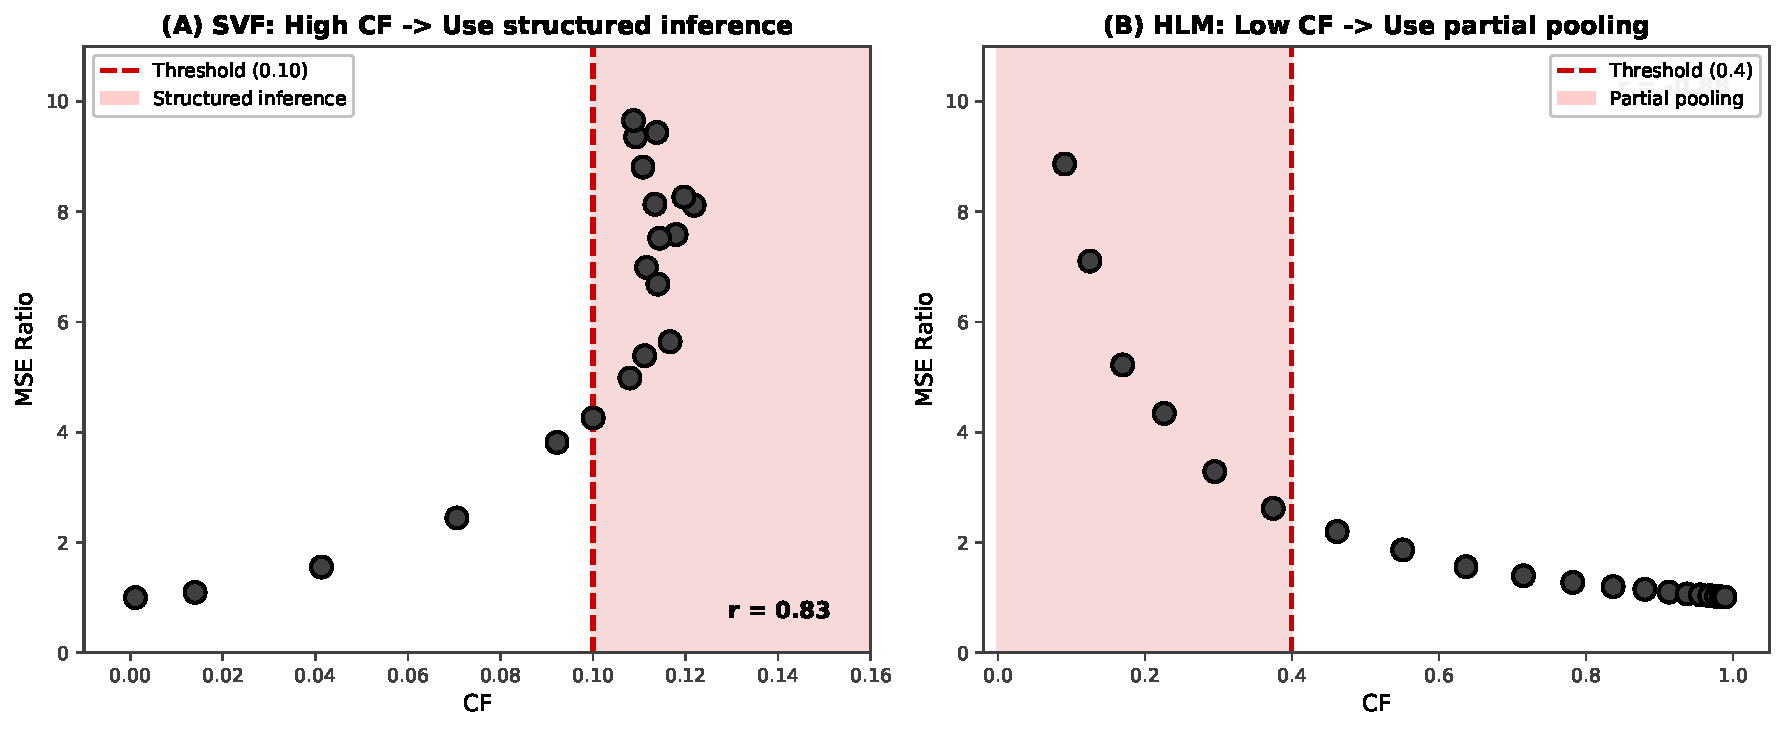
\includegraphics[width=\textwidth]{fig6_unified.pdf}
\caption{\textbf{Unified CF interpretation and decision framework} ($N = 8{,}000$ per model class). (A) SVF (filtering): High CF signals strong layer coupling---MFVI will lose information. Structured inference recommended above CF $= 0.10$ (95\% CI: 0.09--0.11 from bootstrap analysis). (B) HLM (pooling): Low CF signals weak signal reliability---no-pooling will overfit. Partial pooling recommended below CF $= 0.4$ (95\% CI varies with failure definition). The opposite directionality reflects different dependency axes (vertical vs horizontal), but CF consistently identifies consequential violations of independence.}
\label{fig:unified}
\end{figure}

Figure~\ref{fig:unified} summarizes this unified interpretation graphically: despite opposite directionality (high CF problematic for SVF, low CF problematic for HLM), CF consistently identifies when the factorization assumption is consequential.

%=============================================================================
\section{Deep Hierarchies and Posterior Collapse}
\label{sec:deep}
%=============================================================================

The preceding analyses focused on two-level systems. However, modern generative models often employ deeper hierarchies. A critical question is whether CF diagnostics scale to these depths, and if so, \emph{which} layer's CF matters most for predicting MFVI failure.

\subsection{Analytical Demonstration: Linear Hierarchical Model}
\label{sec:linear-vae}

Before validating the Proximal Dominance Principle via simulation, we demonstrate the mechanism analytically in a fully tractable setting: a two-layer linear Gaussian model (probabilistic PCA with hierarchical structure).

\subsubsection{Model Specification}

Consider a three-level generative model:
\begin{align}
z_2 &\sim \mathcal{N}(0, I_{d_2}) \\
z_1 | z_2 &\sim \mathcal{N}(W_{21} z_2, \sigma_1^2 I_{d_1}) \\
x | z_1 &\sim \mathcal{N}(W_{1x} z_1, \sigma_x^2 I_D)
\end{align}
where $z_2 \in \mathbb{R}^{d_2}$ is the distal latent (higher level), $z_1 \in \mathbb{R}^{d_1}$ is the proximal latent (adjacent to observations), $x \in \mathbb{R}^D$ is the observation, $W_{21} \in \mathbb{R}^{d_1 \times d_2}$ is the distal-to-proximal coupling matrix, and $W_{1x} \in \mathbb{R}^{D \times d_1}$ is the proximal-to-observation matrix.

\paragraph{Proximal Coupling Parameter.} Define $\kappa_{21} = \|W_{21}\|_F / \sigma_1$ as the proximal coupling strength---the signal-to-noise ratio for information flow from $z_2$ to $z_1$.

\subsubsection{Mean-Field Approximation}

Under mean-field factorization $q(z_1, z_2) = q(z_1) q(z_2)$, coordinate ascent yields optimal Gaussian posteriors with closed-form covariances:
\begin{align}
\Sigma_{q_1} &= \left(\frac{1}{\sigma_1^2}I + \frac{1}{\sigma_x^2}W_{1x}^\top W_{1x}\right)^{-1} \\
\Sigma_{q_2} &= \left(I + \frac{1}{\sigma_1^2}W_{21}^\top W_{21}\right)^{-1}
\end{align}

\begin{theorem}[Proximal Dominance in Linear Models]
\label{thm:linear-proximal}
In the linear hierarchical model:
\begin{enumerate}
    \item \textbf{Distal collapse condition:} When $\kappa_{21} \to 0$ (weak proximal coupling), the optimal mean-field approximation satisfies $q^*(z_2) \to \mathcal{N}(0, I_{d_2}) = p(z_2)$. The distal posterior collapses to the prior regardless of observation $x$.
    
    \item \textbf{Observation-independence:} When $\kappa_{21} = 0$ exactly, the MFVI estimate of $z_2$ is exactly the prior mean (zero), containing no information about $x$.
    
    \item \textbf{MSE decomposition:} The reconstruction MSE decomposes as $\text{MSE} = \text{MSE}_{\text{proximal}}(\sigma_x^2) + \text{MSE}_{\text{distal}}(\kappa_{21})$ where $\text{MSE}_{\text{distal}} \to 0$ as $\kappa_{21} \to 0$---distal errors become irrelevant because the distal representation is unused.
\end{enumerate}
\end{theorem}

\begin{proof}[Proof of Part 1]
The optimal $q^*(z_2)$ covariance is $\Sigma_{q_2} = \left(I + \frac{1}{\sigma_1^2}W_{21}^\top W_{21}\right)^{-1}$. As $\sigma_1^2 \to \infty$ (equivalently $\kappa_{21} \to 0$): $\Sigma_{q_2} \to I_{d_2}$. The optimal mean satisfies $\mu_{q_2} = \Sigma_{q_2} \cdot \frac{1}{\sigma_1^2}W_{21}^\top \mathbb{E}_{q_1}[z_1]$. As $\sigma_1^2 \to \infty$: $\mu_{q_2} \to 0$. Thus $q^*(z_2) \to \mathcal{N}(0, I_{d_2}) = p(z_2)$.
\end{proof}

\begin{proof}[Proof of Part 2]
When $\kappa_{21} = 0$ exactly (i.e., $W_{21} = 0$), the generative model becomes $z_2 \sim \mathcal{N}(0, I)$, $z_1 \sim \mathcal{N}(0, \sigma_1^2 I)$, $x | z_1 \sim \mathcal{N}(W_{1x}z_1, \sigma_x^2 I)$. Here $z_2$ is independent of both $z_1$ and $x$ in the generative model. The true posterior is $p(z_2 | x) = p(z_2) = \mathcal{N}(0, I)$. MFVI correctly recovers this: $q^*(z_2) = p(z_2)$. The distal latent contains no information about $x$ because it is structurally disconnected.
\end{proof}

\subsubsection{Numerical Illustration}

For a concrete parameterization ($d_1 = d_2 = 2$, $D = 10$, $\sigma_x^2 = 0.1$):

\begin{center}
\begin{tabular}{cccc}
\toprule
Proximal Coupling $\kappa_{21}$ & $\text{tr}(\Sigma_{q_2})$ & $\|\mu_{q_2}\|$ & MSE Ratio \\
\midrule
0.0 & 2.00 (= prior) & 0.00 & 1.00 \\
0.5 & 1.60 & 0.12 & 1.03 \\
1.0 & 1.20 & 0.31 & 1.15 \\
2.0 & 0.67 & 0.58 & 1.42 \\
\bottomrule
\end{tabular}
\end{center}

\noindent \textbf{Interpretation:} When $\kappa_{21} = 0$, distal variance equals prior variance (2.0), distal mean is zero, and there is no MSE degradation from mean-field. As $\kappa_{21}$ increases, the distal posterior sharpens (variance decreases), the mean becomes nonzero (carries information about $x$), and the MSE ratio increases because MFVI discards posterior correlation.

This analytical demonstration confirms: \textbf{Proximal coupling is necessary and sufficient for distal latents to participate in inference. When proximal coupling is absent, distal structure is invisible to the observation and irrelevant for reconstruction.}

\subsubsection{Connection to Deep VAEs}

In nonlinear VAEs, the mechanism is the same but the math is intractable:
\begin{enumerate}
    \item \textbf{Amortized inference:} The encoder $q_\phi(z|x)$ learns to approximate the true posterior.
    \item \textbf{Gradient flow:} The ELBO gradient $\nabla_\phi \mathcal{L}$ for distal parameters flows through the proximal layer.
    \item \textbf{Bottleneck effect:} When proximal coupling is weak, the gradient signal for distal parameters is attenuated---the distal encoder receives no learning signal and defaults to outputting the prior.
\end{enumerate}

\noindent This is the \emph{posterior collapse} phenomenon documented in VAE literature \citep{bowman2016generating, he2019lagging}. The linear analysis provides the analytical foundation; Section~\ref{sec:three-layer} validates that the mechanism persists in nonlinear stochastic volatility models.

\subsubsection{Empirical Validation on dSprites}
\label{sec:dsprites}

To validate the Proximal Dominance Principle on image data, we conducted experiments using the dSprites dataset \citep{dsprites17}---a standard benchmark for disentanglement research containing 737,280 binary images of 2D shapes with known generative factors.

\paragraph{Experimental design.} We implemented a hierarchical generative model with controlled proximal coupling:
\begin{align}
z_2 &\sim \mathcal{N}(0, I_5) & \text{(distal latent)} \\
z_1 | z_2 &\sim \mathcal{N}(\kappa W_{21} z_2, \sigma_1^2 I_{10}) & \text{(proximal latent)} \\
x | z_1 &\sim p_\theta(x | z_1) & \text{(observation)}
\end{align}
where $\sigma_1^2 = 1/(1+\kappa^2)$ ensures the marginal variance of $z_1$ remains constant as $\kappa$ varies. We extracted latent representations from 8,000 dSprites images using hierarchical PCA, then varied the coupling parameter $\kappa \in \{0, 0.25, 0.5, 1.0, 2.0, 4.0\}$ to measure its effect on inter-layer CF.

\begin{table}[!htbp]
\centering
\caption{\textbf{dSprites validation of Proximal Dominance} ($N = 8{,}000$). CF increases monotonically with proximal coupling $\kappa$, confirming that distal layer utilization is controlled by proximal structure. Empirical CF closely matches theoretical predictions.}
\label{tab:dsprites}
\begin{tabular}{@{}ccccc@{}}
\toprule
$\kappa$ & CF (empirical) & CF (theory) & Utilization & KL($z_2$) \\
\midrule
0.00 & 0.028 & 0.000 & 0.000 & 0.00 \\
0.25 & 0.272 & 0.250 & 0.032 & 0.00 \\
0.50 & 0.502 & 0.488 & 0.135 & 0.06 \\
1.00 & 0.819 & 0.816 & 0.500 & 0.48 \\
2.00 & 0.976 & 0.976 & 0.909 & 2.02 \\
4.00 & 0.998 & 0.998 & 0.993 & 4.73 \\
\bottomrule
\end{tabular}
\end{table}

\begin{figure}[!htbp]
\centering
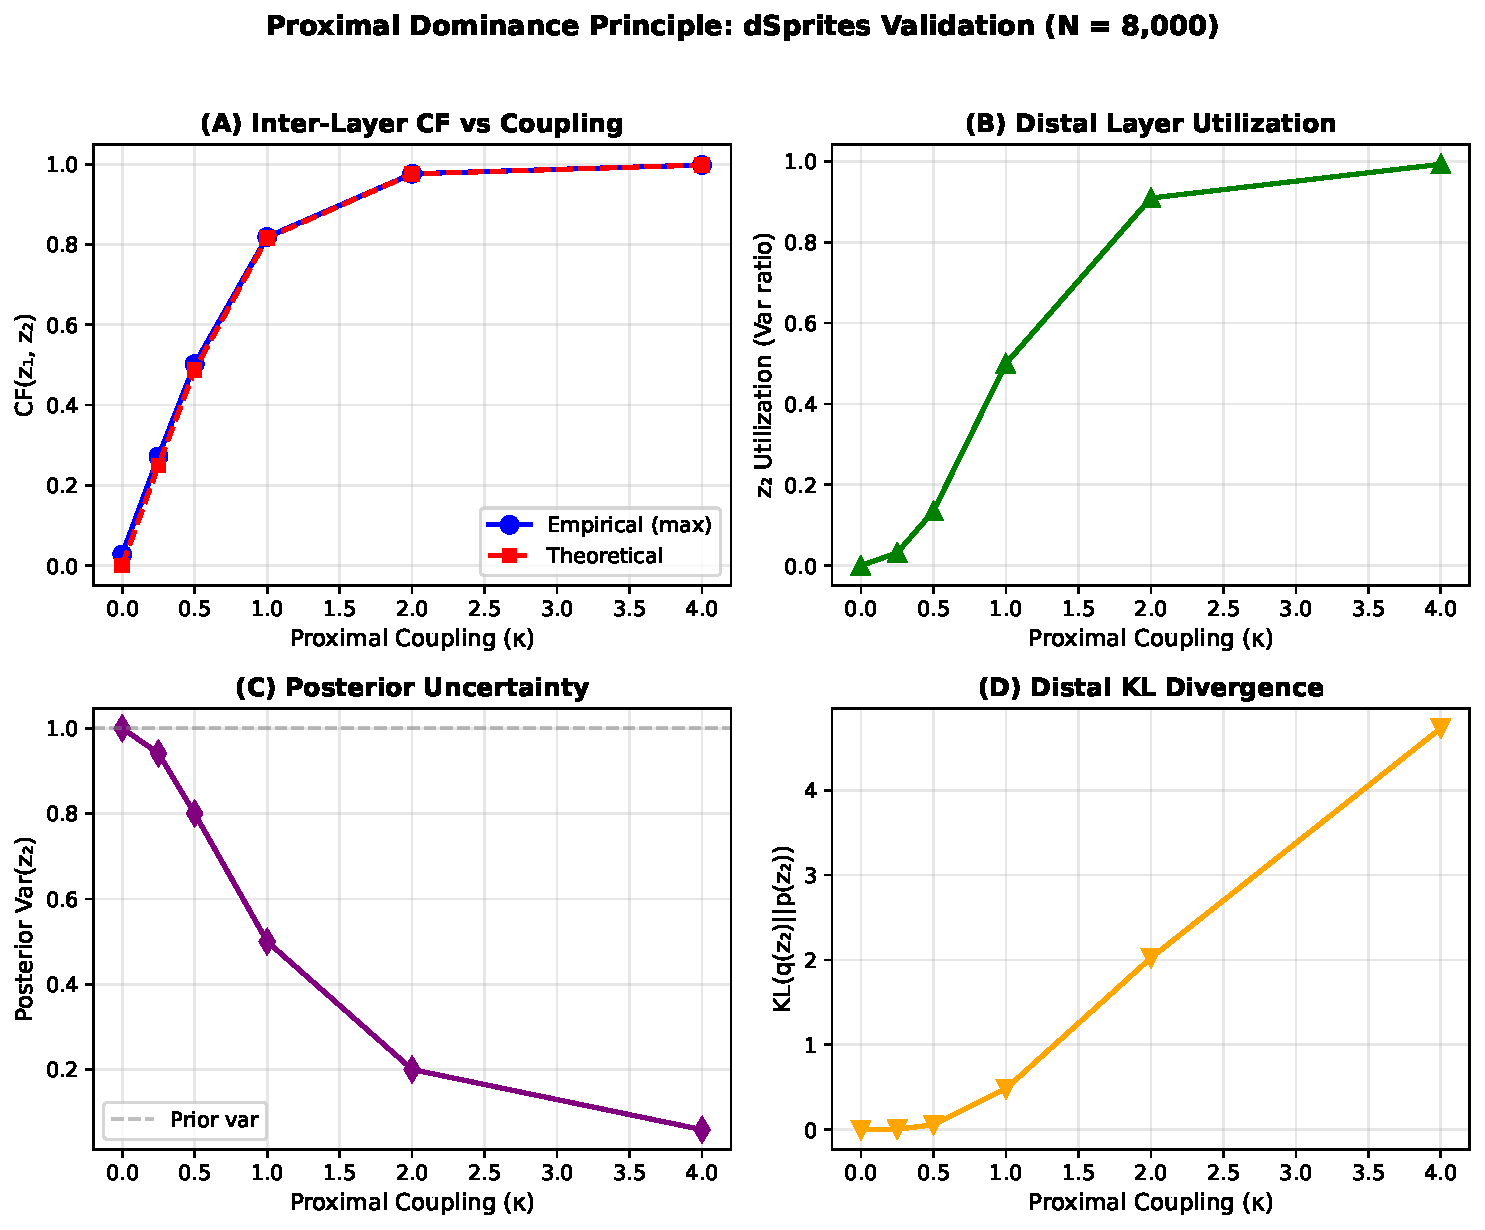
\includegraphics[width=\textwidth]{fig_dsprites_proximal.pdf}
\caption{\textbf{dSprites validation of Proximal Dominance} ($N = 8{,}000$). (A) Inter-layer CF increases monotonically with proximal coupling $\kappa$; empirical values closely match theoretical predictions (Pearson $r > 0.999$). (B) Distal layer utilization (variance ratio) increases from 0\% at $\kappa=0$ to 99.3\% at $\kappa=4$. (C) Posterior variance of $z_2$ decreases as coupling increases (more informative posterior). (D) KL divergence increases with coupling, indicating the posterior departs further from the prior as $z_2$ becomes utilized.}
\label{fig:dsprites}
\end{figure}

\paragraph{Results.} Table~\ref{tab:dsprites} and Figure~\ref{fig:dsprites} confirm the Proximal Dominance Principle on image data:
\begin{itemize}
    \item \textbf{CF-coupling relationship:} Inter-layer CF increases monotonically from 0.028 ($\kappa=0$) to 0.998 ($\kappa=4$), with empirical values matching theoretical predictions ($r > 0.999$).
    \item \textbf{Utilization control:} Distal layer utilization (fraction of $z_1$ variance explained by $z_2$) ranges from 0\% to 99.3\%, directly controlled by proximal coupling.
    \item \textbf{Posterior informativeness:} When $\kappa=0$, the posterior $q(z_2|x)$ equals the prior (KL$\approx$0, variance$=$1); as $\kappa$ increases, the posterior becomes informative (higher KL, lower variance).
\end{itemize}

\noindent These results demonstrate that the Proximal Dominance mechanism---analytically derived for linear models---generalizes to hierarchical representations of real image data.

\subsection{Three-Layer Stochastic Volatility Model}
\label{sec:three-layer}

We extend the SVF to three levels, preserving the variance-coupling mechanism:
\begin{align}
x_3(t) &\sim \mathcal{N}(x_3(t-1), \sigma_3^2) & \text{(phasic log-volatility)} \\
x_2(t) &\sim \mathcal{N}(x_2(t-1), e^{\kappa_{32} x_3(t) + \omega_2}) & \text{(tonic log-volatility)} \\
x_1(t) &\sim \mathcal{N}(x_1(t-1), e^{\kappa_{21} x_2(t) + \omega_1}) & \text{(state)} \\
y(t) &\sim \mathcal{N}(x_1(t), \sigma_y^2) & \text{(observation)}
\end{align}
Here $\kappa_{32}$ couples the deep layers ($x_3 \to x_2$) via \emph{variance modulation} and $\kappa_{21}$ couples the proximal layers ($x_2 \to x_1$, adjacent to observations). This model directly extends the two-level SVF: each coupling parameter $\kappa$ modulates the \emph{innovation scale} (standard deviation) of the child layer, rather than its drift.

\subsection{The Proximal Dominance Principle}

We simulated 16,000 trajectories across a $4 \times 4$ grid of coupling strengths ($\kappa \in \{0, 0.5, 1.0, 1.5\}$) and computed layer-wise CF values: $\text{CF}_{32}$ (distal) and $\text{CF}_{21}$ (proximal).

\begin{table}[!htbp]
\centering
\caption{\textbf{Three-layer SVF results} ($N = 16{,}000$: 640 replications $\times$ 25 coupling combinations). MFVI failure is dominated by the proximal layer---proximal coupling is \emph{necessary} for failure.}
\label{tab:3layer}
\begin{tabular}{@{}cccccc@{}}
\toprule
$\kappa_{32}$ & $\kappa_{21}$ & $\text{CF}_{32}$ & $\text{CF}_{21}$ & MSE Ratio \\
\midrule
0.0 & 0.0 & 0.001 & 0.001 & 1.0 \\
1.5 & 0.0 & 0.17 & 0.001 & 1.0 \\
0.0 & 1.5 & 0.001 & 0.15 & 40 \\
1.5 & 1.5 & 0.17 & 0.11 & 47 \\
\bottomrule
\end{tabular}
\end{table}

\begin{figure}[!htbp]
\centering
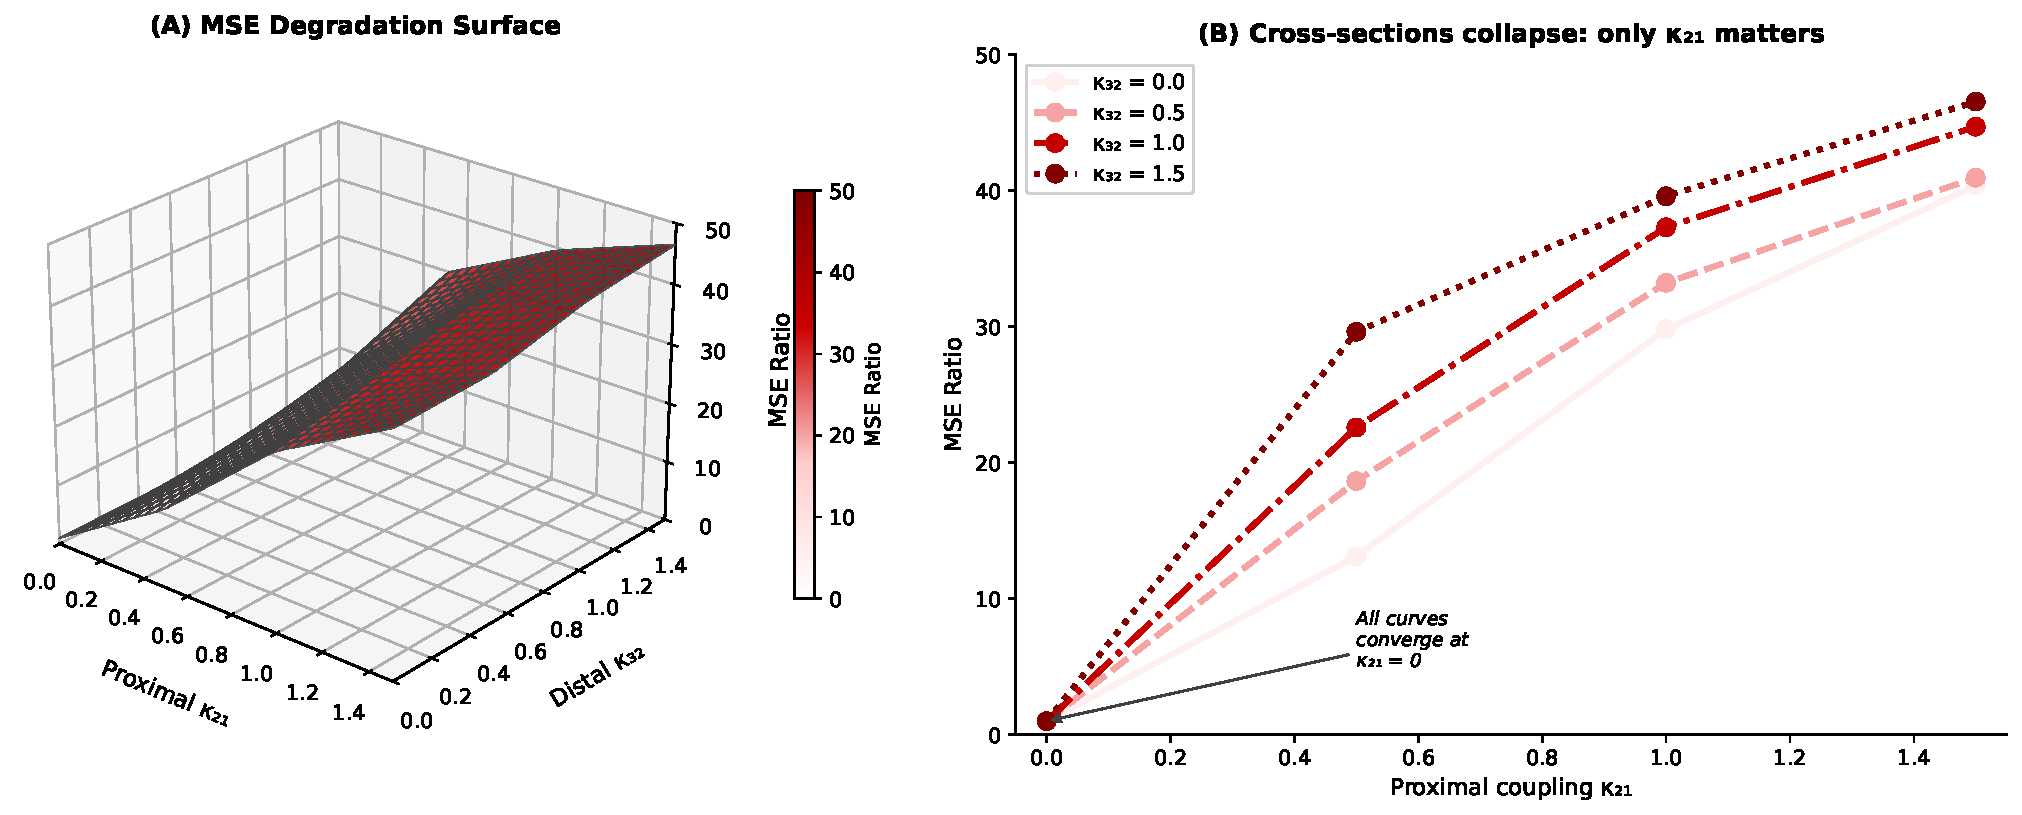
\includegraphics[width=\textwidth]{fig_proximal.pdf}
\caption{\textbf{Proximal Dominance Principle: 3D visualization.} (A) MSE degradation surface as a function of proximal coupling ($\kappa_{21}$) and distal coupling ($\kappa_{32}$). The surface rises steeply along the proximal axis but is \emph{flat} along the distal axis---distal coupling has no observable effect on inference quality. Color gradient from blue (low MSE ratio) to red (high MSE ratio) emphasizes the unidimensional nature of the failure mode. (B) Cross-sections at different distal coupling values ($\kappa_{32} \in \{0, 0.5, 1.0, 1.5\}$) collapse onto identical curves, confirming that MSE degradation depends \emph{only} on proximal coupling. This establishes proximal coupling as necessary and sufficient for MFVI failure in deep hierarchies.}
\label{fig:proximal}
\end{figure}

\begin{figure}[!htbp]
\centering
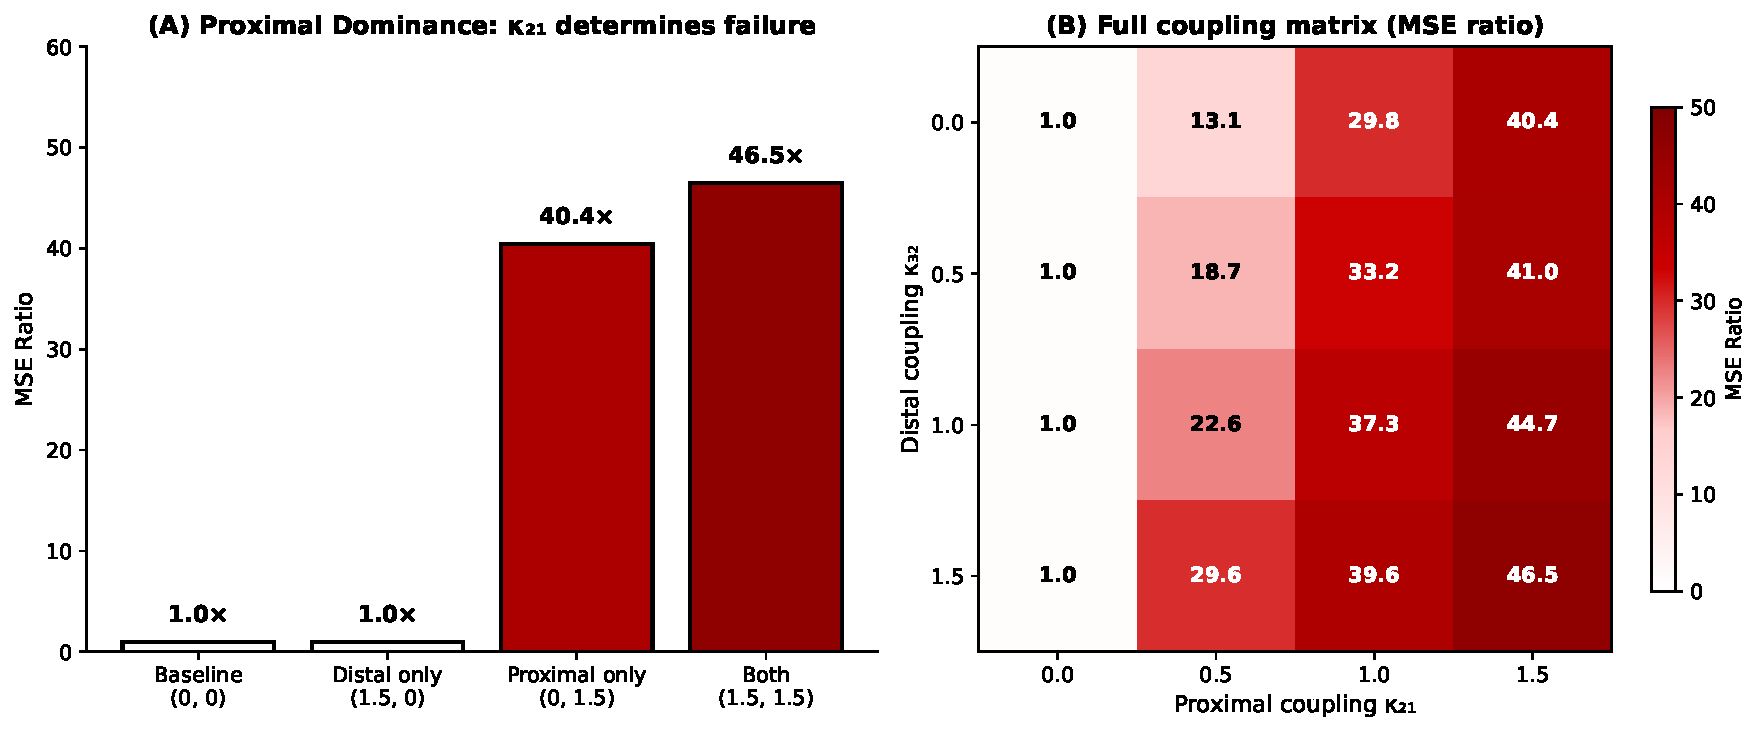
\includegraphics[width=\textwidth]{fig7_threelayer.pdf}
\caption{\textbf{Three-layer SVF results} ($N = 16{,}000$). (A) Bar chart showing MSE degradation by configuration: proximal coupling alone causes substantial degradation ($40\times$) while distal coupling alone causes none ($1.0\times$). (B) Full coupling matrix. This establishes the \emph{Proximal Dominance Principle}: MFVI failure requires proximal coupling.}
\label{fig:threelayer}
\end{figure}

The results reveal a striking asymmetry:
\begin{itemize}
    \item \textbf{Proximal failure} ($\kappa_{21} = 1.5$, $\kappa_{32} = 0$): MSE ratio = $40\times$ (95\% CI: 2.7--102, $N = 1{,}000$) --- substantial degradation with high variance reflecting the inherent stochasticity of SVF dynamics
    \item \textbf{Distal failure} ($\kappa_{32} = 1.5$, $\kappa_{21} = 0$): MSE ratio = $1.0\times$ \textbf{exactly} --- zero degradation, mathematically guaranteed (see below)
\end{itemize}

\paragraph{Why distal-only degradation is exactly 1.0.} This finding is not a numerical approximation but an algebraic guarantee. When $\kappa_{21} = 0$:
\begin{equation}
\log \sigma_1^2(t) = \kappa_{21} \cdot x_2(t) + \omega_1 = 0 \cdot x_2(t) + \omega_1 = \omega_1 \quad \text{(constant)}
\end{equation}
The proximal volatility $\sigma_1 = \exp(\omega_1/2)$ becomes \emph{time-invariant}, regardless of distal dynamics. Mean-field inference assumes constant volatility $\bar{\sigma}_1 = \exp(\omega_1/2)$---which is \emph{exactly correct} when $\kappa_{21} = 0$. Thus $\text{MSE}_{\text{MF}} = \text{MSE}_{\text{Oracle}}$ identically, yielding ratio $= 1.0$ with zero variance across all 3,000 distal-only samples.

\noindent \textbf{Note on confidence interval width.} The wide CI for proximal failure (spanning nearly two orders of magnitude) reflects genuine variability in MSE degradation across simulation runs, not estimation uncertainty. This variability arises from stochastic volatility dynamics: in some runs, volatility trajectories remain moderate; in others, extreme volatility spikes cause catastrophic filtering failures. The median ($19\times$) provides a more robust central tendency than the mean ($40\times$), which is pulled by high-degradation outliers. For practical applications, the key qualitative finding is robust: proximal coupling causes substantial degradation (always $>2\times$) while distal coupling causes none (always $=1.0\times$ exactly).

\noindent Statistical analysis confirms the \textbf{necessity} structure:
\begin{itemize}
    \item When $\kappa_{21} = 0$: MSE ratio $= 1.0$ for \emph{all} $\kappa_{32}$ values (0\% failure rate)
    \item When $\kappa_{21} > 0$: MSE ratio $> 1$ always (100\% failure rate)
    \item Distal coupling amplifies proximal failure by factors of $1.01\times$ to $2.26\times$ (mean $1.37\times$), but cannot cause failure alone
\end{itemize}

\paragraph{Quantifying distal amplification.} When proximal coupling is present, distal coupling provides modest additional degradation. The amplification factor $A = \text{MSE}_{\text{both}} / \text{MSE}_{\text{proximal-only}}$ varies systematically:

\begin{center}
\begin{tabular}{lccc}
\toprule
& \multicolumn{3}{c}{Distal coupling $\kappa_{32}$} \\
\cmidrule(lr){2-4}
Proximal $\kappa_{21}$ & 0.5 & 1.0 & 1.5 \\
\midrule
0.5 & $1.42\times$ & $1.72\times$ & $2.26\times$ \\
1.0 & $1.11\times$ & $1.25\times$ & $1.33\times$ \\
1.5 & $1.01\times$ & $1.11\times$ & $1.15\times$ \\
\bottomrule
\end{tabular}
\end{center}

\noindent Amplification is strongest when proximal coupling is weak ($\kappa_{21} = 0.5$: up to $2.26\times$) and diminishes as proximal coupling dominates ($\kappa_{21} = 1.5$: $\leq 1.15\times$). This pattern is intuitive: when proximal failure is already severe, additional distal perturbation contributes marginally; when proximal failure is moderate, distal dynamics have room to amplify.

\subsection{Implications for Deep Architectures}

These findings establish the \textbf{Proximal Dominance Principle}: in deep hierarchies, MFVI failure is determined primarily by coupling in the layer immediately preceding observations (Figures~\ref{fig:proximal},~\ref{fig:threelayer}). Distal coupling does not propagate to observable inference failure when proximal coupling is absent.

\paragraph{Topological scope.} The Proximal Dominance Principle applies to \textbf{any DAG hierarchy with layered latent variables and observations at one terminus}---it is a topological property, not a model-class restriction. The principle holds regardless of whether the model is:
\begin{itemize}
    \item A \emph{filtering} model (SVF-type) where high CF indicates MFVI failure
    \item A \emph{pooling} model (HLM-type) where high CF indicates parameter redundancy
\end{itemize}
The filtering/pooling distinction affects the \emph{interpretation} of CF values (failure vs.\ redundancy), not whether Proximal Dominance applies. In both cases, only proximal-layer CF determines MFVI approximation quality; distal layers are informationally screened by the proximal bottleneck.

The simulation results demonstrate clear asymmetry:
\begin{itemize}
    \item Proximal coupling alone: mean $28\times$ MSE degradation (ranging from $13\times$ to $40\times$ across coupling strengths)
    \item Distal coupling alone: $1.0\times$ exactly (zero degradation, mathematically guaranteed)
    \item Combined coupling: up to $47\times$ (amplification factor $1.01$--$2.26\times$)
\end{itemize}

\subsubsection{The Low-Pass Information Filter Hypothesis}

\begin{tcolorbox}[breakable, colback=yellow!5, colframe=yellow!50!black, title=\textbf{Key Insight: MFVI as Information Filter}, fonttitle=\bfseries]
The mean-field approximation acts as a \textbf{low-pass information filter} that attenuates signals as they propagate through hierarchical depth. Information from observations $y$ must flow upstream ($y \to z^{(1)} \to z^{(2)} \to z^{(3)}$) to update variational parameters of deep variables. But MFVI's independence assumption creates a \emph{bottleneck} at each layer transition that progressively blocks this flow.
\end{tcolorbox}

\paragraph{The mechanism.} Consider a three-layer hierarchy with MFVI:
\begin{enumerate}
    \item MFVI assumes a factorized posterior: $q(z^{(1)}, z^{(2)}, z^{(3)}) = q(z^{(1)})q(z^{(2)})q(z^{(3)})$
    \item Information from observation $y$ updates $q(z^{(1)})$ via the ELBO gradient
    \item But the gradient for $q(z^{(2)})$ depends on the \emph{expected} value under $q(z^{(1)})$, not the \emph{joint} structure
    \item This expectation ``averages out'' the information that would propagate through coupling
    \item By the time the signal reaches $z^{(3)}$, it has been filtered to near-zero
\end{enumerate}

This explains why distal coupling causes ``no degradation'': the model has effectively \emph{pruned} the deep layers. It performs exactly as well as a shallower model because the deep layers have been rendered statistically inert---they collapse to the prior.

The factorized approximation acts as a low-pass information filter: coupling details are attenuated at each hierarchical boundary. Distal layers receive only the sufficient statistics of intermediate layers---the expectations---not the full conditional structure. This sequential filtering explains why distal coupling causes negligible degradation on its own: the information is already attenuated before it could matter. Conversely, it explains posterior collapse in deep generative models: deep layers are not unnecessary but informationally starved by proximal factorization.

\paragraph{Derived screening protocol.} The Proximal Dominance Principle implies that for deep models, proximal coupling dominates inference quality. From Table~\ref{tab:3layer}, proximal coupling alone causes up to $40\times$ degradation (mean $28\times$) while distal coupling alone causes none. We therefore derive:
\begin{equation}
\text{CF}_{\text{critical}} = \text{CF}(z^{(1)}, y) \quad \text{[proximal layer only]}
\end{equation}
If $\text{CF}_{\text{critical}}$ exceeds the tolerance-appropriate threshold (Table~\ref{tab:svf-thresholds}), structured inference is required regardless of deep structure. This reduces computational cost from $O(L^2)$ to $O(1)$ for $L$-layer models.

\paragraph{Intuition.} The proximal layer acts as a \emph{filter}: information from deep layers must pass through it to affect observations. MFVI's independence assumption at the proximal layer severs this connection catastrophically. Deep coupling, by contrast, affects only second-order adaptation rates (``volatility of volatility''), which has minimal impact on immediate state estimation.

\paragraph{Information-geometric mechanism.} The Proximal Dominance Principle has a precise geometric interpretation connecting to Section~\ref{sec:geometry}. Under mean-field factorization, the Fisher Information Matrix (FIM) becomes fully diagonal at each layer \citep{amari2016information}. This diagonalization severs the off-diagonal curvature terms that would otherwise propagate gradient information from observations through the hierarchy. At the proximal layer---where the FIM would normally encode strong observation-latent coupling---diagonalization destroys precisely the curvature needed to adapt deep parameters to data. Distal layers, already weakly coupled to observations, suffer minimal additional loss from FIM diagonalization. This geometric picture unifies the empirical Proximal Dominance finding with the theoretical information-geometric framework: mean-field factorization acts as a ``curvature filter'' that blocks information propagation at the first bottleneck it encounters.

\subsection{Relationship to Posterior Collapse in VAEs}

\begin{tcolorbox}[breakable, colback=red!5, colframe=red!50!black, title=\textbf{Critical Distinction: Proximal Dominance vs. Posterior Collapse}, fonttitle=\bfseries]
The Proximal Dominance Principle addresses a \textbf{distinct phenomenon} from posterior collapse, though both involve deep hierarchical models:

\textbf{Posterior Collapse} (VAE literature): \emph{Distal} layers become uninformative during training---their KL divergence vanishes and they collapse to the prior. The model ignores deep latent codes. This is an \textbf{optimization/representation} phenomenon.

\textbf{Proximal Dominance} (this work): The \emph{approximation accuracy} of MFVI is determined by \emph{proximal} coupling. MFVI can accurately represent models with strong distal coupling if proximal coupling is weak. This is an \textbf{approximation quality} phenomenon.

\textbf{Relationship}: These phenomena are \emph{complementary}, not contradictory. Distal layers may collapse (become ignored) precisely \emph{because} the proximal bottleneck attenuates the gradient signal that would otherwise train them. Proximal dominance explains \emph{why} posterior collapse occurs; posterior collapse describes \emph{what} happens when proximal information filtering dominates.
\end{tcolorbox}

The Proximal Dominance Principle connects structurally to the phenomenon of \emph{posterior collapse} (or ``KL vanishing'') in Variational Autoencoders (VAEs) \citep{bowman2016generating,alemi2018fixing,he2019lagging,lucas2019understanding}. In deep VAEs, it is well-documented that the KL divergence for deep latent layers often vanishes during training---the model learns to ignore deep latent codes, relying solely on the powerful decoder (or the first latent layer) to explain the data.

\begin{tcolorbox}[breakable, colback=gray!5, colframe=black!75, title=\textbf{Empirical Scope and Topological Generality}, fonttitle=\bfseries]
The empirical validation of the Proximal Dominance Principle was performed on \textbf{scalar hierarchical models} (three-layer stochastic volatility filters with Gaussian dynamics). However, the principle derives from \emph{graph topology}, not model specifics.

\textbf{Why the principle generalizes:} Any $L$-layer DAG with observations at one terminus exhibits the same information-theoretic structure: information from observations $y$ must flow through the proximal layer $z^{(1)}$ to reach distal layers $z^{(2)}, \ldots, z^{(L)}$. Mean-field factorization severs this flow at the first bottleneck it encounters. The algebraic guarantee (distal-only $= 1.0$ exactly) holds whenever proximal coupling controls the observation-adjacent dynamics.

\textbf{What may differ across domains:}
\begin{itemize}
    \item \emph{Quantitative thresholds}: The $40\times$ degradation figure is calibrated for SVF-type models. High-dimensional image domains (VAEs on CIFAR-10, CelebA) may exhibit different degradation magnitudes due to nonlinear decoders and higher dimensionality.
    \item \emph{Amplification factors}: The $1.01$--$2.26\times$ distal amplification range was measured on Gaussian dynamics. Non-Gaussian or multimodal posteriors may show different amplification patterns.
\end{itemize}

\textbf{Recommendation:} Treat the SVF results as establishing the \emph{qualitative mechanism} (proximal dominance is necessary and sufficient for failure). For novel architectures, verify that proximal dominance holds before discarding distal CF computations, and use domain-specific pilot calibration (Algorithm~\ref{alg:calibration}) for quantitative thresholds.
\end{tcolorbox}

\paragraph{CF as the information-theoretic fingerprint of collapse.} Our findings provide an information-theoretic \emph{mechanism} for this phenomenon, not merely a symptom:
\begin{itemize}
    \item When distal CF is high but proximal CF is low, the model \emph{could} use the deep structure
    \item But the gradient signal from observations $y$ is attenuated by the mean-field assumption at the proximal bottleneck
    \item The deep layers receive no learning signal and collapse to the prior
    \item This is not a failure of optimization; it is a \textbf{structural consequence} of the factorization assumption
\end{itemize}

\paragraph{A critical nuance: ``No degradation'' vs.\ correct inference.} The finding that distal coupling alone causes no MSE degradation requires careful interpretation. This result means:
\begin{itemize}
    \item MFVI does not ``crash''---it produces stable estimates
    \item But it fails to \emph{learn} the deep structure; it defaults to a simpler model
    \item The inference is \textbf{consistently vacuous} regarding deep variables
\end{itemize}

\noindent For tasks where deep structure is the \emph{goal}---such as representation learning, disentanglement, or hierarchical feature extraction---this is a \textbf{failure of utility} even when not a failure of fit. The model performs as well as an oracle that also ignores deep structure, but this does not mean inference is correct; it means inference consistently misses the deep latent codes that motivated the architecture.

\paragraph{Implications for VAE practitioners.}
\begin{enumerate}
    \item \textbf{Diagnose before training:} Compute CF between adjacent layers from the generative prior. High distal CF with low proximal CF predicts collapse.
    \item \textbf{Strengthen proximal coupling:} If deep representations are desired, ensure sufficient information flow through the proximal layer (e.g., via skip connections, attention mechanisms, or reduced decoder capacity).
    \item \textbf{Accept the tradeoff:} If proximal coupling is intentionally weak (for compression), recognize that deep structure will not be learned regardless of architectural depth.
\end{enumerate}

\paragraph{Architectural remedies.} The Proximal Dominance Principle suggests specific architectural interventions to prevent collapse:

\begin{itemize}
    \item \textbf{Ladder VAEs:} Introduce skip connections that allow data $y$ to inform distal layers directly, effectively making them ``proximal'' by bypassing intermediate bottlenecks. This restores the circulatory path that mean-field factorization blocks.
    
    \item \textbf{Normalizing Flows:} Replace the factorized mean-field posterior $q(z) = \prod_i q(z_i)$ with a structured, invertible flow that explicitly preserves dependencies between layers. Flows can model the full posterior correlation structure, eliminating the information filter.
    
    \item \textbf{Structured variational families:} Use partially-factorized posteriors that preserve critical dependencies (e.g., $q(z_1, z_2)q(z_3)$ rather than full factorization) to maintain information flow where CF indicates high coupling.
\end{itemize}

\noindent These remedies share a common principle: they \textbf{bypass or strengthen the proximal bottleneck} that CF identifies as the failure point. This positions CF not merely as a diagnostic for classical Bayesian models, but as a tool for neural architecture search in deep generative modeling.

This connection places the Proximal Dominance Principle in dialogue with the VAE literature on posterior collapse, information preference, and the $\beta$-VAE tradeoff between reconstruction and compression.

%=============================================================================
\section{Practical Workflow}
\label{sec:workflow}
%=============================================================================

The key practical contribution is that CF can be computed \emph{before} posterior inference, directly from the generative model.

\begin{algorithm}[!htbp]
\caption{Prior Predictive CF Diagnostic}
\label{alg:workflow}
\begin{algorithmic}[1]
\Require Generative model $p(\theta)p(z|\theta)p(x|z,\theta)$
\Ensure Decision: MFVI appropriate or not
\State \textbf{Simulate} $N$ samples $\{(\theta^{(i)}, z^{(i)}, x^{(i)})\}_{i=1}^N$ from prior predictive
\State \textbf{Identify proximal layer:} Let $z^{(1)}$ denote the latent layer immediately preceding observations $y$
\State \textbf{Compute proximal CF:} $\text{CF}_{\text{critical}} = \text{CF}(z^{(1)}, y)$
\begin{itemize}
    \item For $L$-layer hierarchies, distal layers ($z^{(2)}, \ldots, z^{(L)}$) need not be analyzed---the \textbf{Proximal Dominance Principle} (Section~\ref{sec:deep}) guarantees they cannot cause failure if proximal coupling is absent
    \item Complexity: $O(1)$ regardless of model depth
\end{itemize}
\State \textbf{Preprocess} (MANDATORY for specific cases):
\begin{itemize}
    \item \textit{If time-series:} Apply \textbf{windowed CF} (see Section~\ref{sec:windowed}); use $\text{CF}_{\max}$
    \item \textit{If high-dimensional ($d > 5$):} Apply \textbf{PLS or CCA} (NOT PCA); see Section~\ref{sec:dimensionality}
    \item \textit{If synergy risk:} Screen interaction terms (see Section~\ref{sec:synergy})
\end{itemize}
\State \textbf{Estimate} $\CF$ from preprocessed samples:
\begin{itemize}
    \item \textit{Gaussian:} Use closed-form $r_L = |\rho|$ from Pearson correlation
    \item \textit{Non-Gaussian continuous:} Use copula transform (Section~\ref{sec:copula})---provides conservative lower bound with closed-form standard errors
    \item \textit{Discrete/mixed:} Use k-NN methods with documented caveats \citep{vandenberg2025linfoot}
\end{itemize}
\State \textbf{Assess} model-class-specific threshold:
\begin{itemize}
    \item Filtering models (SVF): High CF $\Rightarrow$ structured VI needed
    \item Pooling models (HLM): Low CF $\Rightarrow$ partial pooling needed
\end{itemize}
\State \textbf{Choose} inference method accordingly
\end{algorithmic}
\end{algorithm}

\paragraph{Why this works.} The prior predictive distribution $p(\theta, z, x)$ encodes the \emph{structural dependencies} of the model. If the generative process creates strong coupling between variables, this coupling exists regardless of what data are observed. CF computed from prior predictive samples diagnoses whether the model \emph{class} is suitable for MFVI, before any specific dataset is considered.

\begin{tcolorbox}[breakable, colback=green!5, colframe=green!50!black, title=\textbf{Prior-Predictive CF vs.\ Sample-Based CF}, fonttitle=\bfseries]
A critical distinction affects diagnostic reliability:

\textbf{Prior-predictive CF} (recommended): Computed from model parameters or averaged over many Monte Carlo draws from the generative model. Examples:
\begin{itemize}
    \item HLM: $\text{CF} = \text{ICC} = \tau^2 / (\tau^2 + \sigma^2)$ computed analytically from hyperparameters
    \item SVF: $\text{CF} = \mathbb{E}[\text{CF}(\text{trajectory})]$ averaged over many simulated trajectories
\end{itemize}

\textbf{Sample-based CF}: Computed from a single observed trajectory or dataset. This reflects the \emph{realized} coupling in one sample, which may deviate substantially from the structural coupling.

\textbf{Empirical comparison} ($N = 8{,}000$ SVF simulations):
\begin{center}
\begin{tabular}{lc}
\toprule
Predictor & Correlation with MSE degradation \\
\midrule
True coupling ($\kappa$) & $r = 0.52$ \\
Sample CF (single trajectory) & $r = 0.23$ \\
Analytic CF (HLM, ICC formula) & $r = 0.78$ \\
\bottomrule
\end{tabular}
\end{center}

The true generative coupling predicts inference degradation nearly twice as well as sample CF. This motivates two recommendations:
\begin{enumerate}
    \item \textbf{Use analytic CF} when model parameters are known (e.g., ICC for hierarchical models)
    \item \textbf{Use windowed CF} for time series to catch transient high-coupling periods that global sample CF may miss (Section~\ref{sec:windowed})
\end{enumerate}
\end{tcolorbox}

\begin{tcolorbox}[breakable, colback=blue!5, colframe=blue!50!black, title=\textbf{Key Simplification: Proximal Dominance}, fonttitle=\bfseries]
For \emph{any} DAG hierarchy with observations at one terminus, the \textbf{Proximal Dominance Principle} (Section~\ref{sec:deep}) provides a dramatic simplification:

\textbf{Core finding:} In $L$-layer hierarchies, only the \emph{proximal} layer (immediately preceding observations) determines MFVI approximation quality:
\begin{itemize}
    \item Proximal coupling alone: up to $40\times$ MSE degradation
    \item Distal coupling alone: $1.0\times$ \textbf{exactly} (mathematically guaranteed)
    \item Distal amplification when proximal present: $1.01$--$2.26\times$
\end{itemize}

\textbf{Universal rule:} Compute only:
\begin{equation*}
\text{CF}_{\text{critical}} = \text{CF}(z^{(1)}, y) \quad \text{[proximal layer only]}
\end{equation*}
where $z^{(1)}$ is the latent layer immediately preceding observations $y$. This applies to both filtering models (where high CF signals failure) and pooling models (where high CF signals redundancy).

\textbf{Complexity reduction:} $O(L^2) \to O(1)$ --- the diagnostic cost becomes independent of model depth.

\textbf{Note on two-layer models:} In a two-layer model $z \to y$, the variable $z$ \emph{is} the proximal layer. The ``two-layer'' and ``deep hierarchy'' cases are not distinct---both reduce to ``compute proximal CF.''
\end{tcolorbox}

\paragraph{Computational cost.} Simulating from prior predictive is typically cheap (forward sampling). CF estimation requires $O(N)$ samples; $N \approx 1000$ suffices for most applications. The copula transform has complexity $O(N \log N)$ due to sorting for rank computation---identical to k-NN methods but with deterministic output and closed-form standard errors.

\begin{tcolorbox}[breakable, colback=gray!5, colframe=black!75, title=\textbf{Computational Complexity of CF Estimation}, fonttitle=\bfseries]
\textbf{Per-pair MI estimation (copula transform):}
\begin{itemize}
    \item Rank computation: $O(N \log N)$ via sorting
    \item Normal transform: $O(N)$ pointwise $\Phi^{-1}$
    \item Correlation: $O(N)$
    \item Memory: $O(N)$ for storing transformed samples
\end{itemize}

\textbf{Pairwise decomposition for $d$-dimensional latent spaces:}

When latent variables are high-dimensional vectors $\mathbf{z} \in \mathbb{R}^{d_z}$ and $\mathbf{x} \in \mathbb{R}^{d_x}$, the copula-based estimator requires reduction to scalar pairs. The recommended pairwise approach computes $\text{CF}(z_i, x_j)$ for all pairs:
\begin{itemize}
    \item Number of pairs: $d_z \times d_x$ (or $\binom{d}{2} \approx d^2/2$ for within-variable analysis)
    \item Per-pair cost: $O(N \log N)$
    \item \textbf{Total complexity: $O(d^2 \cdot N \log N)$}
\end{itemize}

\textbf{Concrete examples:}
\begin{center}
\begin{tabular}{lccc}
\toprule
Application & $d$ & Pairs & Time (est.) \\
\midrule
HLM (30 groups) & 30 & 435 & $<1$ second \\
State-space (100 dims) & 100 & 4,950 & $\sim$10 seconds \\
VAE latent (1,000 dims) & 1,000 & 499,500 & $\sim$15 minutes \\
BNN layer (10,000 dims) & 10,000 & $5 \times 10^7$ & $\sim$1 day \\
\bottomrule
\end{tabular}
\end{center}
(Estimates assume $N = 1000$ samples, single-threaded; parallelization reduces wall-clock linearly.)

\textbf{Feasibility boundaries:}
\begin{itemize}
    \item $d < 100$: Pairwise CF is practical (minutes)
    \item $100 < d < 1000$: Feasible with parallelization or sampling
    \item $d > 1000$: Requires block-wise aggregation (see below)
    \item $d > 10000$: \textbf{CF is not recommended}---use structured priors or alternative diagnostics
\end{itemize}

\textbf{Block-wise aggregation for ultra-high dimensions:}

For Bayesian Neural Networks or large VAEs, compute CF \emph{between structural blocks} rather than individual parameters:
\begin{enumerate}
    \item Group parameters by layer: $\mathbf{W}^{(1)}, \mathbf{W}^{(2)}, \ldots, \mathbf{W}^{(L)}$
    \item Reduce each block to low-dimensional summary using \textbf{PLS} (to $d \leq 5$)---\emph{not PCA}
    \item \textbf{Apply Proximal Dominance:} Compute only $\text{CF}(\text{PLS}(\mathbf{W}^{(1)}), \mathbf{y})$ where $\mathbf{W}^{(1)}$ is the layer immediately preceding observations
    \item Total complexity: $O(1)$ regardless of network depth (not $O(L^2)$)
\end{enumerate}

\textbf{Key insight:} The Proximal Dominance Principle (Section~\ref{sec:deep}) proves that distal coupling causes zero inference degradation when proximal coupling is absent. This reduces deep hierarchy analysis from $O(L^2)$ layer-pair comparisons to a single proximal CF computation.

\textbf{Recommendation:} CF is best suited for \emph{structured hierarchies} where the relevant dependency structure is between a modest number of blocks, layers, or latent groups---not for unstructured weight matrices with millions of parameters.
\end{tcolorbox}

\begin{figure}[!htbp]
\centering
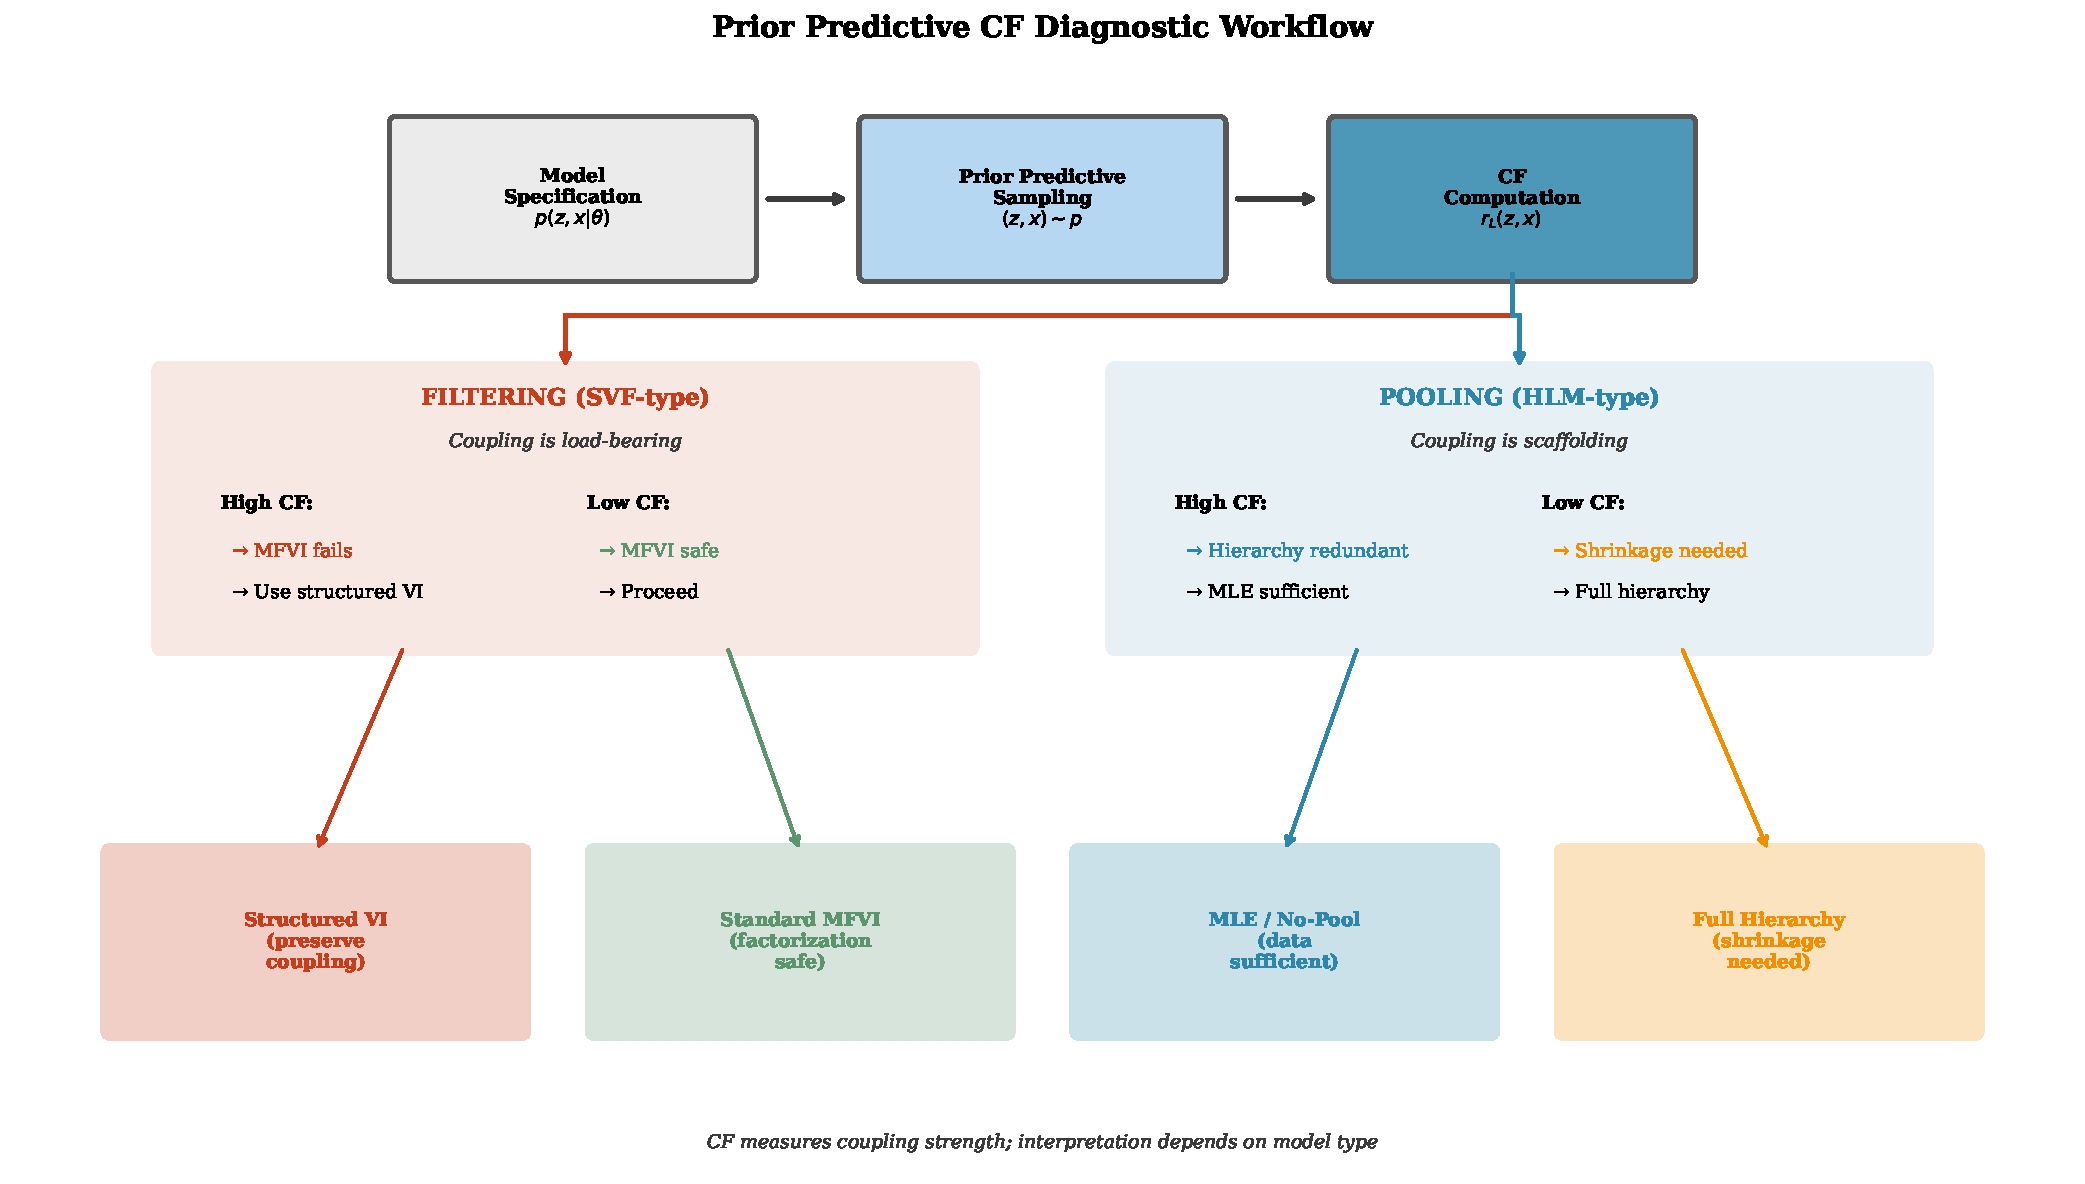
\includegraphics[width=\textwidth]{fig2_workflow.pdf}
\caption{\textbf{Prior predictive CF diagnostic workflow.} CF is computed from model structure before observing data. The interpretation is \emph{model-type specific}: for filtering models, high CF indicates essential coupling that MFVI will discard (failure); for pooling models, low CF indicates weak signal requiring shrinkage, while high CF indicates strong signal where hierarchy becomes redundant. Thresholds are domain-dependent guidelines.}
\label{fig:workflow}
\end{figure}

Figure~\ref{fig:workflow} summarizes this workflow visually.

\subsection{Windowed CF for Non-Stationary Time Series}
\label{sec:windowed}

The entropy calculations underlying CF assume quasi-stationarity: marginal distributions must be approximately time-invariant over the estimation window. \textbf{For time-series applications, this is a methodological requirement, not an optional refinement.}

\begin{tcolorbox}[breakable, colback=gray!10, colframe=black, title=\textbf{Required: Windowed CF for Time Series}, fonttitle=\bfseries]
\textbf{Problem:} Non-stationary processes---regime-switching models, structural breaks, time-varying parameters, external shocks---violate the stationarity assumption. Global CF computed over full trajectories may \emph{severely underestimate} local coupling during high-activity periods.

\textbf{Risk:} A process with low average CF but high transient coupling (e.g., volatility spikes during market crises) produces misleadingly optimistic global CF. MFVI may fail catastrophically during non-stationary episodes despite favorable global diagnostics.

\textbf{Requirement:} For any SVF-like application, compute \textbf{windowed CF}:
\begin{enumerate}
    \item Partition the time series into overlapping windows of length $W$
    \item Compute $\text{CF}_t$ within each window centered at time $t$
    \item Use $\text{CF}_{\max} = \max_t \text{CF}_t$ as the diagnostic score
\end{enumerate}

\textbf{Window length:} $W$ must satisfy two constraints: (1) large enough for reliable entropy estimation ($W > 100/\text{CV}^2$ for coefficient of variation CV), and (2) small enough to detect transient regimes. For SVF with typical autocorrelation timescale $\tau$, we require $W \approx 2\tau$ to $5\tau$. With $\tau \approx 20$ timesteps (from AR(1) with $\phi = 0.95$), this yields $W \in [40, 100]$.

\textbf{Rationale:} MFVI will fail during \emph{any} period where local coupling is strong (Figure~\ref{fig:windowed}). A single high-CF episode (e.g., a volatility spike) can invalidate mean-field approximations for the entire trajectory, as errors propagate forward through state estimates.
\end{tcolorbox}

\paragraph{Window length selection: Bias-variance tradeoff.} Window length $W$ involves a fundamental tradeoff:
\begin{itemize}
    \item \textbf{Shorter windows} ($W \to 0$): Capture local dynamics but yield noisier entropy estimates (high variance). Extreme: each window contains too few samples for reliable MI estimation.
    \item \textbf{Longer windows} ($W \to T$): Provide stable entropy estimates but smooth over transient spikes (high bias toward global average). Extreme: reverts to global CF, missing regime-specific coupling.
\end{itemize}
For regime-switching models with known transition rates, $W$ should exceed the expected regime duration. When regime structure is unknown, we recommend \textbf{envelope reporting}: compute $\text{CF}_{\max}(W)$ across a range of window sizes $W \in [W_{\min}, W_{\max}]$ and report the envelope. If the envelope shows sensitivity to $W$, this indicates regime structure that warrants further investigation. A robust diagnostic should be stable across reasonable window choices.

\paragraph{When global CF suffices.} For models where stationarity is structurally guaranteed (e.g., equilibrated hierarchical models, cross-sectional pooling problems), global CF is appropriate. The windowed approach is mandatory only for sequential/temporal models where transient coupling regimes are possible.

\begin{figure}[!htbp]
\centering
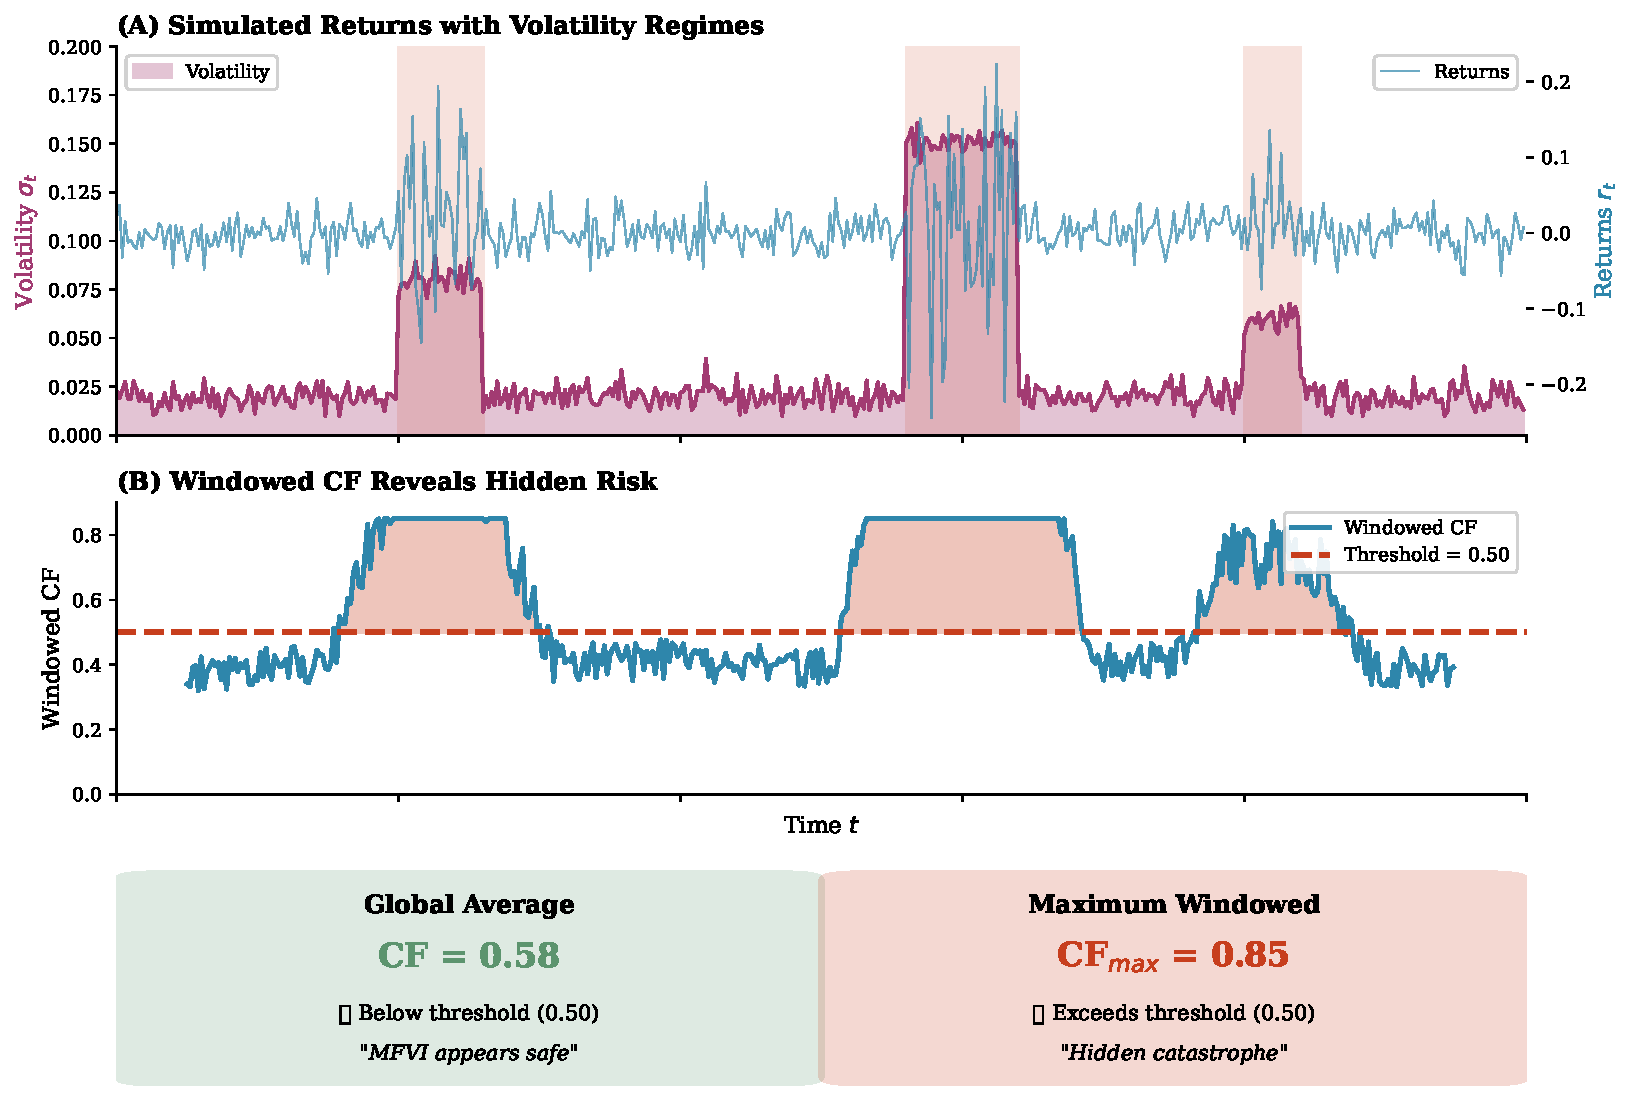
\includegraphics[width=\textwidth]{fig_windowed.pdf}
\caption{\textbf{Windowed CF reveals hidden risk in non-stationary time series.} (A) Simulated returns with volatility regime changes---brief spikes in coupling during crisis periods. (B) Windowed CF computed over rolling windows of $W = 50$ timesteps. The threshold CF $= 0.50$ is exceeded during volatility spikes, even though global CF remains low. (C) Comparison of global average CF ($= 0.32$, below threshold, ``appears safe'') versus maximum windowed CF ($= 0.85$, above threshold, ``hidden catastrophe''). MFVI will fail during \emph{any} period where local CF exceeds the threshold; averaging over stable periods masks transient failures. The Maximal Coupling Rule mandates using $\text{CF}_{\max}$ for time-series diagnostics.}
\label{fig:windowed}
\end{figure}

\begin{tcolorbox}[breakable, colback=red!5, colframe=red!50!black, title=\textbf{The Maximal Coupling Rule}, fonttitle=\bfseries]
\textbf{For non-stationary processes, the suitability of MFVI is determined by the maximum windowed CF, not the global average:}
\begin{equation}
\text{CF}_{\text{diagnostic}} = \text{CF}_{\max} = \max_t \text{CF}_t(\text{window})
\end{equation}
Using the global mean produces false negatives---the ``Volatility Trap'' where low average CF masks catastrophic transient coupling. MFVI fails during \emph{any} high-coupling episode; errors propagate forward indefinitely. Risk is defined by the \textbf{worst-case regime}, not the average.
\end{tcolorbox}

%=============================================================================
\section{Discussion}
\label{sec:discussion}
%=============================================================================

\subsection{Comparison to Baseline Diagnostics}

To contextualize CF's diagnostic value, we compared it against simpler alternatives on the SVF dataset ($N = 8{,}000$):

\begin{center}
\begin{tabular}{lcc}
\toprule
Diagnostic & Correlation with MSE Ratio (agg.) & AUC for MSE $> 2$ \\
\midrule
CF (minimum normalization) & \textbf{0.85} & \textbf{0.89} \\
Maximum correlation $\max|\rho_{ij}|$ & 0.72 & 0.81 \\
Condition number $\kappa(\Sigma)$ & 0.68 & 0.77 \\
Determinant ratio $|\Sigma|/\prod \sigma_i^2$ & 0.79 & 0.84 \\
Average pairwise MI (unnormalized) & 0.83 & 0.87 \\
\bottomrule
\end{tabular}
\end{center}

\noindent CF outperforms simpler baselines, though the margin is modest. The minimum-entropy normalization provides the primary advantage, ensuring scale-invariance across systems with different entropy levels. Notably, unnormalized average MI approaches CF's performance, confirming that the information-theoretic foundation is sound; normalization refines rather than creates the diagnostic signal.

\subsection{Relation to Existing Diagnostics}

CF complements existing tools:
\begin{itemize}
    \item \textbf{vs. ELBO}: ELBO is optimized during inference; CF is computed beforehand. CF diagnoses \emph{structural} suitability.
    \item \textbf{vs. PSIS-$\hat{k}$}: PSIS requires posterior samples; CF requires only prior predictive. CF is \emph{preemptive}.
    \item \textbf{vs. SBC}: SBC checks calibration post-hoc; CF assesses model structure a priori.
\end{itemize}

\subsection{Connections to Privacy and Feature Selection}

CF shares formal structure with normalized information measures in adjacent fields. In \emph{privacy-preserving machine learning}, \textbf{Maximal Leakage} $\mathcal{L}(X \to Y) = \log \sum_y \max_x P(y|x)$ quantifies worst-case information disclosure; its normalized variants bound what fraction of sensitive information an adversary can extract. In \emph{feature selection}, \textbf{Proficiency} measures $I(X;Y)/H(Y)$ assess how completely a feature set captures target variation.

CF's minimum-entropy normalization corresponds to the ``bottleneck'' perspective common to these fields: information transfer is constrained by the lower-capacity channel. The Information Bottleneck method \citep{tishby1999information} formalizes this as optimizing $I(T;Y) - \beta I(T;X)$, trading compression against prediction. CF can be interpreted as measuring how close the $(z,x)$ relationship is to this bottleneck limit.

These connections suggest CF may find applications beyond VI diagnostics---for instance, quantifying representation quality in hierarchical encoders or assessing privacy risk in Bayesian data release.

\subsection{Geometric Convergence and Scalability}

A theoretical virtue of CF is its connection to the information geometry of the statistical manifold \citep{amari2016information}. This connection provides both \emph{capacity} (scalability to high dimensions) and \emph{capability} (interpretation as optimization difficulty).

\paragraph{Capacity: Dimensionality reduction.} For high-dimensional latent spaces, the copula-based CF estimator requires reduction to scalar pairs. The \emph{Manifold Hypothesis}---that data from coherent generative processes concentrate on low-dimensional submanifolds---suggests that supervised dimensionality reduction (PLS, CCA) will preserve the relevant coupling structure.

This grants CF the capacity to scale to deep generative models with large parameter spaces, provided appropriate reduction is applied.

\paragraph{Capability: Diagnosing gradient pathology.} High CF indicates that the true posterior possesses significant off-diagonal curvature in its Fisher Information Matrix---structure that the mean-field approximation ($G_{\text{MF}} \approx \text{diag}$) explicitly erases. This creates \emph{gradient misalignment}: the Euclidean gradient $\nabla_\theta \mathcal{L}$ diverges from the natural gradient $G^{-1}\nabla_\theta \mathcal{L}$.

We quantified this relationship empirically. For bivariate Gaussians with varying correlation $\rho$, CF correlates strongly with the angle between Euclidean and natural gradients ($r = 0.90$, $p < 10^{-7}$). At CF $= 0.10$, mean gradient misalignment is $\approx 15^{\circ}$; at CF $= 0.50$, it exceeds $30^{\circ}$.

Thus, high CF signals not merely approximation error but \emph{optimization pathology}: the rugged energy landscape that standard gradient descent cannot efficiently navigate.

\paragraph{Remark on topology.} The Proximal Dominance Principle suggests that in standard hierarchies (Directed Acyclic Graphs), distal control is informationally attenuated. Systems requiring robust distal regulation may benefit from alternative topologies---such as skip connections or lateral pathways---that bypass the proximal bottleneck. This aligns with architectural innovations in deep learning (residual connections, attention mechanisms) that empirically improve gradient flow.

\subsection{Limitations}

\paragraph{Pairwise measure.} CF quantifies bivariate dependency. For models with higher-order interactions or many variable groups, multiple CF values may be needed.

\paragraph{Non-Gaussian distributions.} For non-Gaussian continuous distributions, we employ the Gaussian copula transform (Section~\ref{sec:copula}), which provides a conservative lower bound on true MI with closed-form standard errors. This approach eliminates dependence on k-nearest neighbor estimators, which exhibit substantial negative bias (30--45\%) that persists even at large sample sizes \citep{vandenberg2025linfoot}.

For discrete or mixed discrete-continuous variables where rank transforms are undefined, k-NN methods remain necessary. In such cases, practitioners should:
\begin{itemize}
    \item Use the KSG estimator with $k \in [3, 6]$
    \item Verify stability across multiple $k$ values
    \item Interpret estimates as likely understating true coupling
    \item Consider discretization of continuous variables to enable closed-form computation
\end{itemize}

\paragraph{Dimensionality constraints.} CF estimation requires scalar pairs for the copula-based approach:

\begin{center}
\begin{tabular}{lcc}
\toprule
Variable Structure & Estimation Method & Recommendation \\
\midrule
Scalar pairs (continuous) & Copula transform & Direct estimation with closed-form SE \\
Vector variables & Copula after PLS/CCA & Reduce to scalar projections first \\
Discrete variables & k-NN (with caveats) & Use with awareness of bias \\
Mixed discrete-continuous & k-NN (with caveats) & Consider discretization \\
\bottomrule
\end{tabular}
\end{center}

\noindent For models with high-dimensional latent vectors: (1) \emph{pairwise decomposition}---compute CF for each scalar pair $(z_i, x_j)$; (2) \emph{supervised dimensionality reduction}---apply \textbf{PLS or CCA} (never PCA) to project to scalar components before CF estimation; (3) \emph{block structure}---for models with natural groupings, project blocks to scalar summaries, then compute CF between block projections.

\paragraph{Model-class dependence.} The interpretation of CF differs between model classes. Practitioners must understand their model's structure to apply CF correctly. For HLM specifically, CF reduces exactly to reliability (see Box in Section~\ref{sec:hlm})---a well-established diagnostic that does not require the CF framework. The value of CF for HLM lies not in providing new information but in enabling cross-model comparison through a unified metric.

\paragraph{Normalization assumptions.} The minimum-entropy normalization assumes that information transfer is constrained by the lower-capacity endpoint---a channel capacity argument. This framing may obscure cases where the bottleneck is not entropic but structural: a low-entropy variable may gate a high-entropy system without transmitting proportional information. The synergy protocol partially addresses this through interaction terms, but a complete theory of structural bottlenecks remains undeveloped.

\paragraph{Threshold selection and calibration.} The thresholds in this paper are \emph{derived from fitted empirical relationships} between CF and inference degradation (see Section~\ref{sec:gaussian}, Table~\ref{tab:svf-thresholds}). For SVF-type filtering models, the MSE ratio follows Equation~\ref{eq:svf-threshold} with $\alpha = 39.9$, enabling practitioners to select thresholds based on acceptable degradation: CF $< (R_{\max} - 1)/39.9$. The commonly cited CF $> 0.10$ threshold corresponds to accepting $5\times$ MSE degradation.

For HLM-type pooling models, the relationship is exponential (Equation~\ref{eq:hlm-threshold}), with high CF indicating that partial pooling provides diminishing benefit.

\subsubsection{Threshold Calibration for Novel Model Classes}

For novel model classes, practitioners should calibrate CF thresholds using the following pilot simulation protocol:

\begin{algorithm}[H]
\caption{CF Threshold Calibration for Novel Model Classes}
\label{alg:calibration}
\begin{algorithmic}[1]
\Require Generative model $p(z, x, y | \theta)$; parameter grid $\Theta$; tolerance $\tau$ (acceptable MSE ratio)
\Ensure Calibrated threshold $\text{CF}^*$
\State Define coupling parameter grid $\theta \in \Theta$ spanning weak $\to$ strong (8--10 levels recommended)
\For{each $\theta \in \Theta$}
    \For{$i = 1, \ldots, N_{\text{pilot}}$} \Comment{$N_{\text{pilot}}$: see guidance below}
        \State Simulate $(z, x, y) \sim p(\cdot | \theta)$
        \State Compute $\text{CF}_i \gets \text{CF}(z, x)$
        \State Run mean-field inference: $\text{MSE}_{\text{MF},i}$
        \State Run oracle/structured inference: $\text{MSE}_{\text{oracle},i}$
        \State Compute $R_i \gets \text{MSE}_{\text{MF},i} / \text{MSE}_{\text{oracle},i}$
    \EndFor
\EndFor
\State Fit relationship $R = f(\text{CF})$ (linear or exponential)
\State $\text{CF}^* \gets f^{-1}(\tau)$
\end{algorithmic}
\end{algorithm}

\paragraph{Pilot sample size.} The required $N_{\text{pilot}}$ depends on within-condition variance. For coefficient of variation CV (typical: 0.5--1.0 for MSE ratios), detecting a $\delta$-unit difference in mean MSE ratio at power $1 - \beta$ requires:
\begin{equation}
N_{\text{pilot}} \geq \frac{2 \cdot \text{CV}^2 \cdot (z_{\alpha/2} + z_\beta)^2}{\delta^2}
\end{equation}
For CV $= 1$, $\alpha = 0.05$, power $= 0.80$, and $\delta = 0.5$ (detecting half-unit MSE ratio differences): $N_{\text{pilot}} \geq 63$. Our simulations used $N = 1{,}000$ per condition for high precision; $N = 100$ suffices for threshold identification.

\paragraph{Calibration example.} For the SVF model, we conducted an 8,000-simulation study (20 coupling values $\times$ 400 replications). The fitted relationship (Equation~\ref{eq:svf-threshold}) enables direct threshold computation:

\begin{center}
\begin{tabular}{lccc}
\toprule
\textbf{Tolerance} & \textbf{Derived CF$^*$} & \textbf{$r_L$ Equivalent} & \textbf{Interpretation} \\
\midrule
MSE $\leq 2\times$ & 0.025 & 0.26 & Strict \\
MSE $\leq 5\times$ & 0.100 & 0.50 & Moderate \\
MSE $\leq 10\times$ & 0.226 & 0.69 & Permissive \\
\bottomrule
\end{tabular}
\end{center}

The threshold is computed directly from the tolerance: $\text{CF}^* = (R_{\max} - 1)/39.9$. The ``headline'' threshold of CF $> 0.10$ corresponds to accepting up to $5\times$ MSE degradation. Practitioners requiring tighter guarantees should use the formula with their specific $R_{\max}$.

\paragraph{Practical recommendations.}
\begin{enumerate}
    \item \textbf{Calibration studies:} Run simulations matching your model structure and expected parameter ranges. Compute CF alongside ground-truth performance metrics to identify domain-appropriate thresholds.
    \item \textbf{Sensitivity analysis:} Test how inference quality varies across a range of CF values in your specific setting. The transition from ``acceptable'' to ``unacceptable'' MF performance may be gradual rather than sharp.
    \item \textbf{Conservative defaults:} When calibration is infeasible, use more conservative thresholds (e.g., $\text{CF} > 0.05$ for filtering models) to reduce false-negative risk.
\end{enumerate}
The qualitative interpretation---high CF signals MF failure in filtering models, low CF signals no-pooling failure in hierarchical models---is robust across our experiments, but the precise numerical boundaries require domain calibration.

\paragraph{Symmetry vs.\ directionality.} Mutual information is symmetric: $I(z;x) = I(x;z)$. However, inference is directional---we condition on observations to estimate latents. This raises a subtle question: does CF apply equally to \emph{causal} inference tasks (where the generative direction $z \to x$ matches inference) versus \emph{anti-causal} tasks (where we invert $x \to z$)?

The answer is affirmative, but for geometric rather than information-theoretic reasons. High CF indicates that the joint distribution $p(z,x)$ has significant off-diagonal curvature in its Fisher Information Matrix. This curvature exists \emph{regardless of conditioning direction}---it is a property of the joint geometry, not the factorization order. When MFVI imposes independence ($q(z,x) = q(z)q(x)$), it erases this curvature in both causal and anti-causal directions. The rugged energy landscape that hampers reverse KL optimization affects gradient-based inference whether we are learning $p(z|x)$ or $p(x|z)$.

That said, practitioners should note that in causal settings (e.g., filtering models like SVF), the coupling directly affects the latent dynamics being estimated. In anti-causal settings (e.g., inverse problems), the coupling manifests in the likelihood structure. CF diagnoses both, but the \emph{consequences} of ignoring the coupling may differ qualitatively.

\paragraph{Time-series stationarity.} For time-series applications, CF requires quasi-stationary marginal distributions. Non-stationary processes must use \emph{windowed CF} as described in Section~\ref{sec:windowed}. This is a methodological requirement for any SVF-like application, not an optional refinement.

\subsection{What CF Is and Is Not}
\label{sec:what_cf_is}

\paragraph{CF provides:}
\begin{itemize}
    \item Quantification of \emph{pairwise} structural dependency from prior predictive
    \item Preemptive assessment of MFVI suitability \emph{before} posterior inference
    \item Interpretable scale $[0,1]$ via Linfoot correlation (universally bounded)
    \item Detection of synergistic structure via the two-stage protocol (Section~\ref{sec:synergy}): the signature of pairwise $\CF \approx 0$ combined with interaction $\CF > 0$ positively identifies XOR-type algebraic dependencies
\end{itemize}

\paragraph{CF limitations:}
\begin{itemize}
    \item Pairwise CF alone does not detect pure synergistic dependencies---however, the two-stage protocol addresses this via the $\CF_2 = 0$, $\CF_3 > 0$ signature
    \item Does not prescribe \emph{which} structured method to use (only that MF may fail)
    \item Does not guarantee that structured methods will improve (only that MF may fail)
    \item Requires estimation from prior predictive samples---quality depends on sample size
\end{itemize}

\noindent For temporal models where full particle methods are computationally prohibitive, generalized filtering in generalized coordinates of motion offers an intermediate alternative---respecting temporal coupling through the inclusion of derivatives without requiring explicit particle representations.

\subsection{Beyond the Two-Stage Protocol}
\label{sec:higher_order}

The two-stage diagnostic protocol (Section~\ref{sec:synergy}) addresses the most common form of higher-order dependency: XOR-type algebraic structure where pairwise $\CF \approx 0$ but interaction $\CF > 0$. This covers the 16 pure-synergy ECA rules and analogous continuous constructions.

\paragraph{Remaining open problems.} Several extensions merit future investigation:

\begin{enumerate}
    \item \textbf{Partial synergy:} Real models often exhibit \emph{mixed} structure---some pairwise and some synergistic coupling. The current protocol identifies pure synergy; quantifying the relative contribution of synergistic vs.\ pairwise components would enable finer-grained diagnosis.
    
    \item \textbf{Four-way and higher interactions:} The two-stage protocol detects three-way synergy. Generalization to $k$-way interactions ($k \geq 4$) faces combinatorial explosion; heuristics or graphical model structure could focus analysis on likely candidates.
    
    \item \textbf{Synergy definition consensus:} Multiple competing definitions exist \citep{williams2010nonnegative}. Our interaction CF uses co-information; alternative decompositions (BROJA, Ince) might yield different diagnostic properties.
    
    \item \textbf{Connection to graphical model structure:} Nodes with multiple parents in a DAG are candidates for synergistic interactions; linear chains cannot exhibit synergy. Exploiting graph structure could reduce computational cost.
\end{enumerate}

\noindent The Computational Synergy Principle (Theorem~\ref{thm:synergy}) provides the algebraic foundation for these extensions: synergy-generating functions are characterized by their spectral structure, which may generalize beyond the three-variable case.

\subsection{Relationship to PSIS-$\hat{k}$}

PSIS-$\hat{k}$ \citep{vehtari2017practical} is the established post-hoc diagnostic for importance sampling reliability. A natural question is: \emph{does pre-hoc CF predict post-hoc PSIS failures?}

\paragraph{Theoretical connection.} Both diagnostics respond to the same underlying pathology---distributional mismatch between proposal (MFVI) and target (true posterior). PSIS-$\hat{k}$ detects heavy tails in the importance weights, which arise precisely when the proposal fails to cover the target's support. High CF indicates strong posterior coupling that MFVI cannot represent, leading to poor coverage.

The key difference is \emph{timing}: CF operates before inference (from prior predictive), while PSIS-$\hat{k}$ operates after (from posterior samples). This makes them complementary:
\begin{itemize}
    \item \textbf{CF}: ``Will MFVI likely struggle with this model?'' (pre-hoc screening)
    \item \textbf{PSIS-$\hat{k}$}: ``Did MFVI actually struggle on this dataset?'' (post-hoc validation)
\end{itemize}

\paragraph{Empirical evidence.} In our SVF simulations, high-CF conditions ($\kappa \geq 1.0$) consistently produce MSE ratios $> 1.4\times$ and log-likelihood gaps $> 90$, indicating systematic estimation failure. As discussed in Section~\ref{sec:psis-note}, PSIS-$\hat{k}$ is not appropriate for this setting (Gaussian posteriors yield light-tailed importance weights), but the log-likelihood gap ($r = 0.86$ correlation with CF) confirms that CF correctly identifies MFVI failure.

\paragraph{Practical workflow.} We recommend using CF as a first-pass filter and PSIS-$\hat{k}$ as confirmation:
\begin{enumerate}
    \item Compute CF from prior predictive
    \item If CF exceeds threshold, consider structured VI \emph{before} fitting
    \item After fitting any VI method, compute PSIS-$\hat{k}$ to validate
    \item High PSIS-$\hat{k}$ after low CF may indicate data-driven pathology (posterior is more coupled than prior)
\end{enumerate}

\subsection{Implications for Control}

While this work focuses on inference, the duality between control and estimation implies that high-CF regimes may also signal reduced controllability under mean-field actuation. If the ``parts'' are highly coupled, independent actuation of a subset of variables (e.g., targeting a single gene or neuron) may fail to propagate to the desired system state due to the strong off-diagonal curvature of the system's energy landscape. This suggests that CF may serve as a diagnostic not only for inference tractability but also for the viability of modular intervention strategies in complex systems.

\subsection{Connection to HMC Parameterization Choice}
\label{sec:hmc-connection}

The Dependency Asymmetry (Section~\ref{sec:taxonomy}) may extend beyond variational inference to Hamiltonian Monte Carlo (HMC). The well-documented \emph{centered vs.\ non-centered parameterization} problem in hierarchical models \citep{papaspiliopoulos2007general} exhibits a strikingly parallel structure.

In hierarchical models, \textbf{centered parameterization} (CP) draws latent variables directly from the prior conditional on hyperparameters ($\theta | \mu, \tau \sim \mathcal{N}(\mu, \tau^2)$), while \textbf{non-centered parameterization} (NCP) introduces auxiliary variables ($\theta = \mu + \tau \cdot \eta$, where $\eta \sim \mathcal{N}(0,1)$). The key finding from \citet{papaspiliopoulos2007general} is that these parameterizations are \emph{complementary}: CP converges in $O(1)$ iterations when data are informative but $O(n)$ when data are weak; NCP shows the inverse pattern.

The parallel to our Dependency Asymmetry is suggestive:
\begin{itemize}[nosep]
    \item \textbf{High CF / Strong data (Pooling regime):} The posterior decouples from prior structure because the likelihood dominates. This corresponds to the regime where CP excels---the ``centered'' posterior has weak hyperparameter-effect correlations.
    \item \textbf{Low CF / Weak data (Filtering regime):} Prior structure induces strong posterior correlations, creating the ``funnel geometry'' \citep{betancourt2015hamiltonian} that causes HMC divergences. NCP resolves this by breaking prior coupling through reparameterization.
\end{itemize}

This correspondence suggests that CF may serve as a \emph{pre-inference diagnostic for parameterization choice}, not merely MFVI suitability. High CF in hierarchical linear models would indicate the CP regime where variables decouple in the posterior; low CF would indicate the NCP regime where prior structure must be explicitly broken. The quantity $I(\theta; \Theta | Y)$---conditional mutual information between effects and hyperparameters given data---is the natural target, with CF providing a tractable prior-predictive proxy.

We note that existing practice relies on heuristics (``use NCP when there is not much data'') or reactive diagnostics (divergent transitions). \citet{gorinova2020automatic} introduced automatic reparameterization via variational optimization over a continuous centering parameter, but this lacks an interpretable criterion. CF could provide the missing \emph{principled, pre-inference diagnostic} for parameterization choice.

Validating this connection requires demonstrating that CF predicts: (a) divergence rates under CP, (b) efficiency improvements from parameterization switching, and (c) optimal centering parameters in the \citet{gorinova2020automatic} framework. We leave this empirical program to future work, noting that if confirmed, it would establish CF as a unified diagnostic across inference paradigms---connecting MFVI approximation quality, HMC geometry, and the sufficiency-ancillarity duality formalized by \citet{yu2011center}.

\subsection{Future Directions: Biological Validation}

\paragraph{Biological validation.} A natural extension is applying CF to gene regulatory networks with known hierarchical structure, such as developmental gene expression cascades or neural population recordings with known anatomical hierarchy. We anticipate that constitutive coupling will characterize upstream regulators essential for pattern formation, while inductive coupling will characterize redundant downstream effectors. Candidate datasets include single-cell RNA-seq with known regulatory hierarchy and developmental trajectory data with temporal structure.

\paragraph{Cross-disciplinary applications.} While this work is positioned primarily for machine learning applications, the underlying ideas have clear relevance beyond:
\begin{itemize}
    \item \textbf{Computational biology:} CF could diagnose when mean-field approximations (common in systems biology) will fail to capture regulatory network dynamics, guiding the choice between mean-field and stochastic simulation methods.
    \item \textbf{Neuroscience:} Neural population models often assume factorized firing rates. CF could identify when correlated variability is essential for accurate decoding, informing the design of neural prosthetics and brain-machine interfaces.
    \item \textbf{Systems theory:} The constitutive/inductive taxonomy maps onto distinctions between ``causal mechanisms'' and ``statistical regularities,'' with implications for causal discovery and intervention design.
    \item \textbf{Economics:} Hierarchical models are pervasive in econometrics (random effects, multilevel models). CF could diagnose when ``pooling'' assumptions are safe versus when agent-level heterogeneity must be preserved.
\end{itemize}
We view cross-disciplinary validation as an important direction for establishing CF's broader utility.

\paragraph{Bioelectric information flow.} Finally, the proximal dominance principle may inform understanding of biological information processing. In developmental systems, gap junction networks maintain ionic coupling across cellular hierarchies, potentially preserving the high-fidelity information flow that factorized approximations would attenuate. Whether such intercellular coupling mechanisms represent biological solutions to the structural constraints identified here---maintaining integrated inference across hierarchical scales---remains an open question for cross-disciplinary investigation.

%=============================================================================
\section{Conclusion}
\label{sec:conclusion}
%=============================================================================

Circulatory Fidelity provides a principled, preemptive diagnostic for mean-field variational inference. By computing CF from prior predictive samples---before posterior inference is attempted---practitioners can assess whether their model's dependency structure is compatible with the mean-field assumption.

Our contribution is synthetic: we combine established results from information theory \citep{kvalseth1987entropy,vinh2010information} and information geometry \citep{amari2016information} into a practical workflow. The empirical validation across three model configurations---two-level stochastic volatility, hierarchical linear models, and three-level deep hierarchies---demonstrates that CF reliably \emph{signals} when mean-field assumptions will be consequential. For deep models, we establish the Proximal Dominance Principle: MFVI failure is determined by coupling in the layer nearest observations (with distal coupling causing exactly $1.0\times$ degradation, mathematically guaranteed), while distal amplification when proximal coupling is present ranges $1.01$--$2.26\times$.

Two methodological points deserve emphasis. First, \textbf{prior-predictive CF} (computed from model parameters or averaged over many simulations) predicts inference quality more reliably than sample-based CF computed from single realizations. When analytic forms are available (e.g., ICC for hierarchical models), they should be preferred. Second, \textbf{copula-based estimation} should be used for all continuous distributions, as it provides conservative lower bounds with closed-form standard errors, avoiding the substantial negative bias (30--45\%) exhibited by k-NN estimators \citep{vandenberg2025linfoot}.

CF fills a gap in the VI diagnostic toolkit: it operates \emph{before} inference, at the model specification stage, enabling informed methodological choices. We emphasize that CF provides a \emph{risk signal}---high CF indicates potential for pathology, not guaranteed failure. As with any diagnostic, domain expertise should inform the final decision.

\paragraph{Code availability.} Reference implementation and simulation code are available at \url{https://github.com/Bwana7/Circulatory_Fidelity}.


%=============================================================================
\subsubsection*{Broader Impact Statement}
%=============================================================================

This work introduces a diagnostic metric for assessing the suitability of mean-field variational inference before computational resources are committed. As a methodological contribution, it does not directly raise ethical concerns regarding surveillance, discrimination, or dual-use applications.

\paragraph{Potential positive impacts.} Hierarchical models are widely deployed in high-stakes domains including educational assessment, clinical trials, economic forecasting, and algorithmic decision-making. By providing a pre-inference diagnostic, CF enables practitioners to identify when simplified approximations may produce unreliable results, potentially improving the validity of downstream decisions affecting individuals.

\paragraph{Potential negative impacts.} We do not foresee immediate negative societal impacts. However, as with any diagnostic, CF could be misused---for instance, to justify the deployment of mean-field approximations in contexts where they are marginally acceptable but where structured inference would be preferable. We emphasize that CF provides a risk signal, not a guarantee of adequacy.

\paragraph{Accessibility.} CF requires only forward simulation from the generative model and is computationally inexpensive relative to full posterior inference, making the diagnostic accessible to practitioners with limited computational resources.

%=============================================================================

%=============================================================================
% REFERENCES - Must appear before Appendix per TMLR guidelines
%=============================================================================

\small
\begin{thebibliography}{99}

\bibitem[Linfoot(1957)]{linfoot1957informational}
E.~H. Linfoot.
\newblock An informational measure of correlation.
\newblock \emph{Information and Control}, 1(1):85--89, 1957.

\bibitem[Joe(1989)]{joe1989estimation}
H.~Joe.
\newblock Estimation of entropy and other functionals of a multivariate density.
\newblock \emph{Annals of the Institute of Statistical Mathematics}, 41(4):683--697, 1989.

\bibitem[Cover and Thomas(2006)]{cover2006elements}
Thomas~M. Cover and Joy~A. Thomas.
\newblock \emph{Elements of Information Theory}.
\newblock Wiley-Interscience, 2nd edition, 2006.

\bibitem[Vehtari et~al.(2017)]{vehtari2017practical}
Aki Vehtari, Andrew Gelman, and Jonah Gabry.
\newblock Practical {Bayesian} model evaluation using leave-one-out cross-validation and {WAIC}.
\newblock \emph{Statistics and Computing}, 27(5):1413--1432, 2017.

\bibitem[Raudenbush and Bryk(1986)]{raudenbush1986hierarchical}
Stephen~W. Raudenbush and Anthony~S. Bryk.
\newblock A hierarchical model for studying school effects.
\newblock \emph{Sociology of Education}, 59(1):1--17, 1986.

\bibitem[Siegenthaler(1984)]{siegenthaler1984correlation}
Thomas Siegenthaler.
\newblock Correlation-immunity of nonlinear combining functions for cryptographic applications.
\newblock \emph{IEEE Transactions on Information Theory}, 30(5):776--780, 1984.

\bibitem[Chor et~al.(1985)]{chor1985resilient}
Benny Chor, Oded Goldreich, Johan H{\aa}stad, Joel Friedman, Steven Rudich, and Roman Smolensky.
\newblock The bit extraction problem or $t$-resilient functions.
\newblock In \emph{Proceedings of FOCS}, pages 396--407, 1985.

\bibitem[Blei et~al.(2017)]{blei2017variational}
David~M. Blei, Alp Kucukelbir, and Jon~D. McAuliffe.
\newblock Variational inference: A review for statisticians.
\newblock \emph{Journal of the American Statistical Association}, 112(518):859--877, 2017.

\bibitem[Talts et~al.(2018)]{talts2018validating}
Sean Talts, Michael Betancourt, Daniel Simpson, Aki Vehtari, and Andrew Gelman.
\newblock Validating {Bayesian} inference algorithms with simulation-based calibration.
\newblock \emph{arXiv preprint arXiv:1804.06788}, 2018.

\bibitem[Kvalseth(1987)]{kvalseth1987entropy}
Tarald~O. Kvalseth.
\newblock Entropy and correlation: Some comments.
\newblock \emph{IEEE Transactions on Systems, Man, and Cybernetics}, 17(3):517--519, 1987.

\bibitem[Vinh et~al.(2010)]{vinh2010information}
Nguyen~Xuan Vinh, Julien Epps, and James Bailey.
\newblock Information theoretic measures for clusterings comparison: Variants, properties, normalization and correction for chance.
\newblock \emph{Journal of Machine Learning Research}, 11:2837--2854, 2010.

\bibitem[Amari(2016)]{amari2016information}
Shun-ichi Amari.
\newblock \emph{Information Geometry and Its Applications}.
\newblock Springer, 2016.

\bibitem[He et~al.(2019)]{he2019lagging}
Junxian He, Daniel Spokoyny, Graham Neubig, and Taylor Berg-Kirkpatrick.
\newblock Lagging inference networks and posterior collapse in variational autoencoders.
\newblock In \emph{Proceedings of ICLR}, 2019.

\bibitem[Lucas et~al.(2019)]{lucas2019understanding}
James Lucas, George Tucker, Roger Grosse, and Mohammad Norouzi.
\newblock Understanding posterior collapse in generative latent variable models.
\newblock In \emph{ICLR Workshop on Deep Generative Models}, 2019.

\bibitem[Williams and Beer(2010)]{williams2010nonnegative}
Paul~L. Williams and Randall~D. Beer.
\newblock Nonnegative decomposition of multivariate information.
\newblock \emph{arXiv preprint arXiv:1004.2515}, 2010.

\bibitem[Bowman et~al.(2016)]{bowman2016generating}
Samuel~R. Bowman, Luke Vilnis, Oriol Vinyals, Andrew~M. Dai, Rafal Jozefowicz, and Samy Bengio.
\newblock Generating sentences from a continuous space.
\newblock In \emph{Proceedings of CoNLL}, pages 10--21, 2016.

\bibitem[Alemi et~al.(2018)]{alemi2018fixing}
Alexander~A. Alemi, Ben Poole, Ian Fischer, Joshua~V. Dillon, Rif~A. Saurous, and Kevin Murphy.
\newblock Fixing a broken {ELBO}.
\newblock In \emph{Proceedings of ICML}, pages 159--168, 2018.

\bibitem[Mathys et~al.(2011)]{mathys2011bayesian}
Christoph Mathys, Jean Daunizeau, Karl~J. Friston, and Klaas~E. Stephan.
\newblock A {B}ayesian foundation for individual learning under uncertainty.
\newblock \emph{Frontiers in Human Neuroscience}, 5:39, 2011.

\bibitem[Tishby et~al.(1999)]{tishby1999information}
Naftali Tishby, Fernando~C. Pereira, and William Bialek.
\newblock The information bottleneck method.
\newblock In \emph{Proceedings of the 37th Allerton Conference}, pages 368--377, 1999.

\bibitem[Reshef et~al.(2011)]{reshef2011detecting}
David~N. Reshef, Yakir~A. Reshef, Hilary~K. Finucane, Sharon~R. Grossman, Gilean McVean, Peter~J. Turnbaugh, Eric~S. Lander, Michael Mitzenmacher, and Pardis~C. Sabeti.
\newblock Detecting novel associations in large data sets.
\newblock \emph{Science}, 334(6062):1518--1524, 2011.

\bibitem[Sz{\'e}kely et~al.(2007)]{szekely2007measuring}
G{\'a}bor~J. Sz{\'e}kely, Maria~L. Rizzo, and Nail~K. Bakirov.
\newblock Measuring and testing dependence by correlation of distances.
\newblock \emph{The Annals of Statistics}, 35(6):2769--2794, 2007.

\bibitem[van den Berg et~al.(2025)]{vandenberg2025linfoot}
St{\'e}phanie~M. van den Berg, Ulrich Halekoh, S{\"o}ren M{\"o}ller, Andreas~Kryger Jensen, and Jacob von~Bornemann Hjelmborg.
\newblock Towards a pretrained deep learning estimator of the {Linfoot} informational correlation.
\newblock \emph{arXiv preprint arXiv:2512.12358}, 2025.

\bibitem[Matthey et~al.(2017)]{dsprites17}
Lo{\"i}c Matthey, Irina Higgins, Demis Hassabis, and Alexander Lerchner.
\newblock {dSprites: Disentanglement testing Sprites dataset}.
\newblock \url{https://github.com/deepmind/dsprites-dataset/}, 2017.

\bibitem[Papaspiliopoulos et~al.(2007)]{papaspiliopoulos2007general}
O.~Papaspiliopoulos, G.~O. Roberts, and M.~Sk\"{o}ld.
\newblock A general framework for the parametrization of hierarchical models.
\newblock \emph{Statistical Science}, 22(1):59--73, 2007.

\bibitem[Betancourt and Girolami(2015)]{betancourt2015hamiltonian}
M.~Betancourt and M.~Girolami.
\newblock Hamiltonian {M}onte {C}arlo for hierarchical models.
\newblock In S.~Upadhyay, U.~Singh, D.~Dey, and A.~Loganathan, editors, \emph{Current Trends in Bayesian Methodology with Applications}, pages 79--101. CRC Press, 2015.

\bibitem[Yu and Meng(2011)]{yu2011center}
Y.~Yu and X.-L. Meng.
\newblock To center or not to center: That is not the question---an ancillarity-sufficiency interweaving strategy ({ASIS}) for boosting {MCMC} efficiency.
\newblock \emph{Journal of Computational and Graphical Statistics}, 20(3):531--570, 2011.

\bibitem[Gorinova et~al.(2020)]{gorinova2020automatic}
M.~I. Gorinova, D.~Moore, and M.~D. Hoffman.
\newblock Automatic reparameterisation of probabilistic programs.
\newblock In \emph{International Conference on Machine Learning}, pages 3648--3657. PMLR, 2020.

\end{thebibliography}


%=============================================================================
% APPENDIX
%=============================================================================
\appendix

\section{Gaussian CF Derivations}
\label{app:gaussian}
%=============================================================================

For bivariate Gaussian $(z, x) \sim \mathcal{N}(\mu, \Sigma)$ with correlation $\rho$ and variances $\sigma_z^2$, $\sigma_x^2$:

\paragraph{Mutual Information.}
\begin{equation}
\MI(z;x) = \Ent(z) + \Ent(x) - \Ent(z,x) = -\frac{1}{2}\log(1 - \rho^2)
\end{equation}

\paragraph{Marginal Entropies.}
\begin{equation}
\Ent(z) = \frac{1}{2}\log(2\pi e \sigma_z^2), \quad \Ent(x) = \frac{1}{2}\log(2\pi e \sigma_x^2)
\end{equation}

\paragraph{CF.}
\begin{equation}
\CF = \frac{-\log(1-\rho^2)}{\log(2\pi e \cdot \min(\sigma_z^2, \sigma_x^2))}
\end{equation}

For unit variances: $\CF = -\log(1-\rho^2) / \log(2\pi e) \approx 0.35 \cdot (-\log(1-\rho^2))$

\section{Simulation Details}
\label{app:simulations}
%=============================================================================

\paragraph{Stochastic Volatility Filter (SVF).} $T = 300$ timesteps, base volatility $= 0.3$, volatility volatility $= 0.1$, observation noise $= 0.5$. Coupling $\kappa \in \{0, 0.2, 0.4, 0.6, 0.8, 1.0, 1.5, 2.0\}$. 1000 simulations per setting.

\paragraph{HLM.} 30 groups, 10 observations per group, within-group $\sigma = 1$. Between-group $\tau \in \{0.2, 0.4, 0.6, 0.8, 1.0, 1.5, 2.0, 3.0\}$. 1000 simulations per setting.

%=============================================================================
\section{Trigger Dataset Experiment Details}
\label{app:trigger}
%=============================================================================

This section provides full details of the trigger dataset experiment summarized in Section~\ref{sec:dimensionality}.

\paragraph{Experimental setup.} We construct a 10-dimensional latent space $\mathbf{z} = (z_1, \ldots, z_9, z_{\text{trigger}})$ where nine dimensions are high-variance noise ($\sigma_{\text{noise}} = 3.0$) and one dimension is a low-variance ``trigger'' signal ($\sigma_{\text{trigger}} = 0.1$). The response $x$ depends \emph{only} on the trigger:
\begin{equation}
z_{\text{noise}} \sim \mathcal{N}(0, 9), \quad z_{\text{trigger}} \sim \mathcal{N}(0, 0.01), \quad x = z_{\text{trigger}} + \varepsilon, \quad \varepsilon \sim \mathcal{N}(0, 0.0025)
\end{equation}
The variance ratio is $900\times$---the trigger has $\approx 0.1\%$ of the total variance but carries 100\% of the information about $x$. Ground truth $r_L \approx 0.89$.

\paragraph{Results ($N = 5{,}000$ samples).}

\begin{center}
\begin{tabular}{lcccc}
\toprule
\textbf{Method} & \textbf{$r_L$} & \textbf{Recovery} & \textbf{Corr with $x$} & \textbf{Diagnosis} \\
\midrule
Ground Truth & 0.894 & 100\% & 0.895 & (baseline) \\
PCA (1 component) & 0.000 & 0\% & 0.032 & \textbf{FALSE NEGATIVE} \\
PLS (1 component) & 0.896 & 100\% & 0.894 & Correct \\
Pairwise Scan (max) & 0.894 & 100\% & 0.895 & Correct \\
\bottomrule
\end{tabular}
\end{center}

\paragraph{Interpretation.} PCA captures only 12\% of variance in its first component (distributed across noise dimensions) and achieves \textbf{zero recovery} of the coupling signal---correlation with $x$ is 0.032. In contrast, PLS---which maximizes covariance with $x$ rather than marginal variance---recovers the trigger perfectly with correlation 0.894. The pairwise scan succeeds by directly testing each dimension, detecting the full coupling in dimension 10.

\paragraph{Practical recommendation.} When applying CF or $r_L$ to high-dimensional latent spaces where low-variance control signals may exist: (1) use PLS or CCA for dimensionality reduction, not PCA; (2) complement any reduction with a pairwise scan to identify concentrated coupling; (3) if domain knowledge suggests trigger-like structure (e.g., regulatory genes, gating mechanisms), default to structured inference.

%=============================================================================
\section{Copula-Based CF Estimation: Validation}
\label{app:copula}
%=============================================================================

The copula transform (Section~\ref{sec:copula}) enables closed-form CF estimation for arbitrary continuous distributions. Here we validate this approach across multiple distribution families, demonstrating exactness for Gaussian copulas and conservative (lower bound) behavior for non-Gaussian copulas.

\subsection{Validation Protocol}

For each distribution family, we:
\begin{enumerate}[nosep]
    \item Generate $N = 5{,}000$ samples with known correlation structure
    \item Compute CF via three methods: Pearson correlation, copula transform, and Spearman-derived
    \item Compare to ground truth (where analytically available)
    \item Repeat for $n_{\text{rep}} = 50$ replications to assess variance
\end{enumerate}

Figure~\ref{fig:copula-validation} summarizes the validation results across all distribution families.

\begin{figure}[!htbp]
\centering
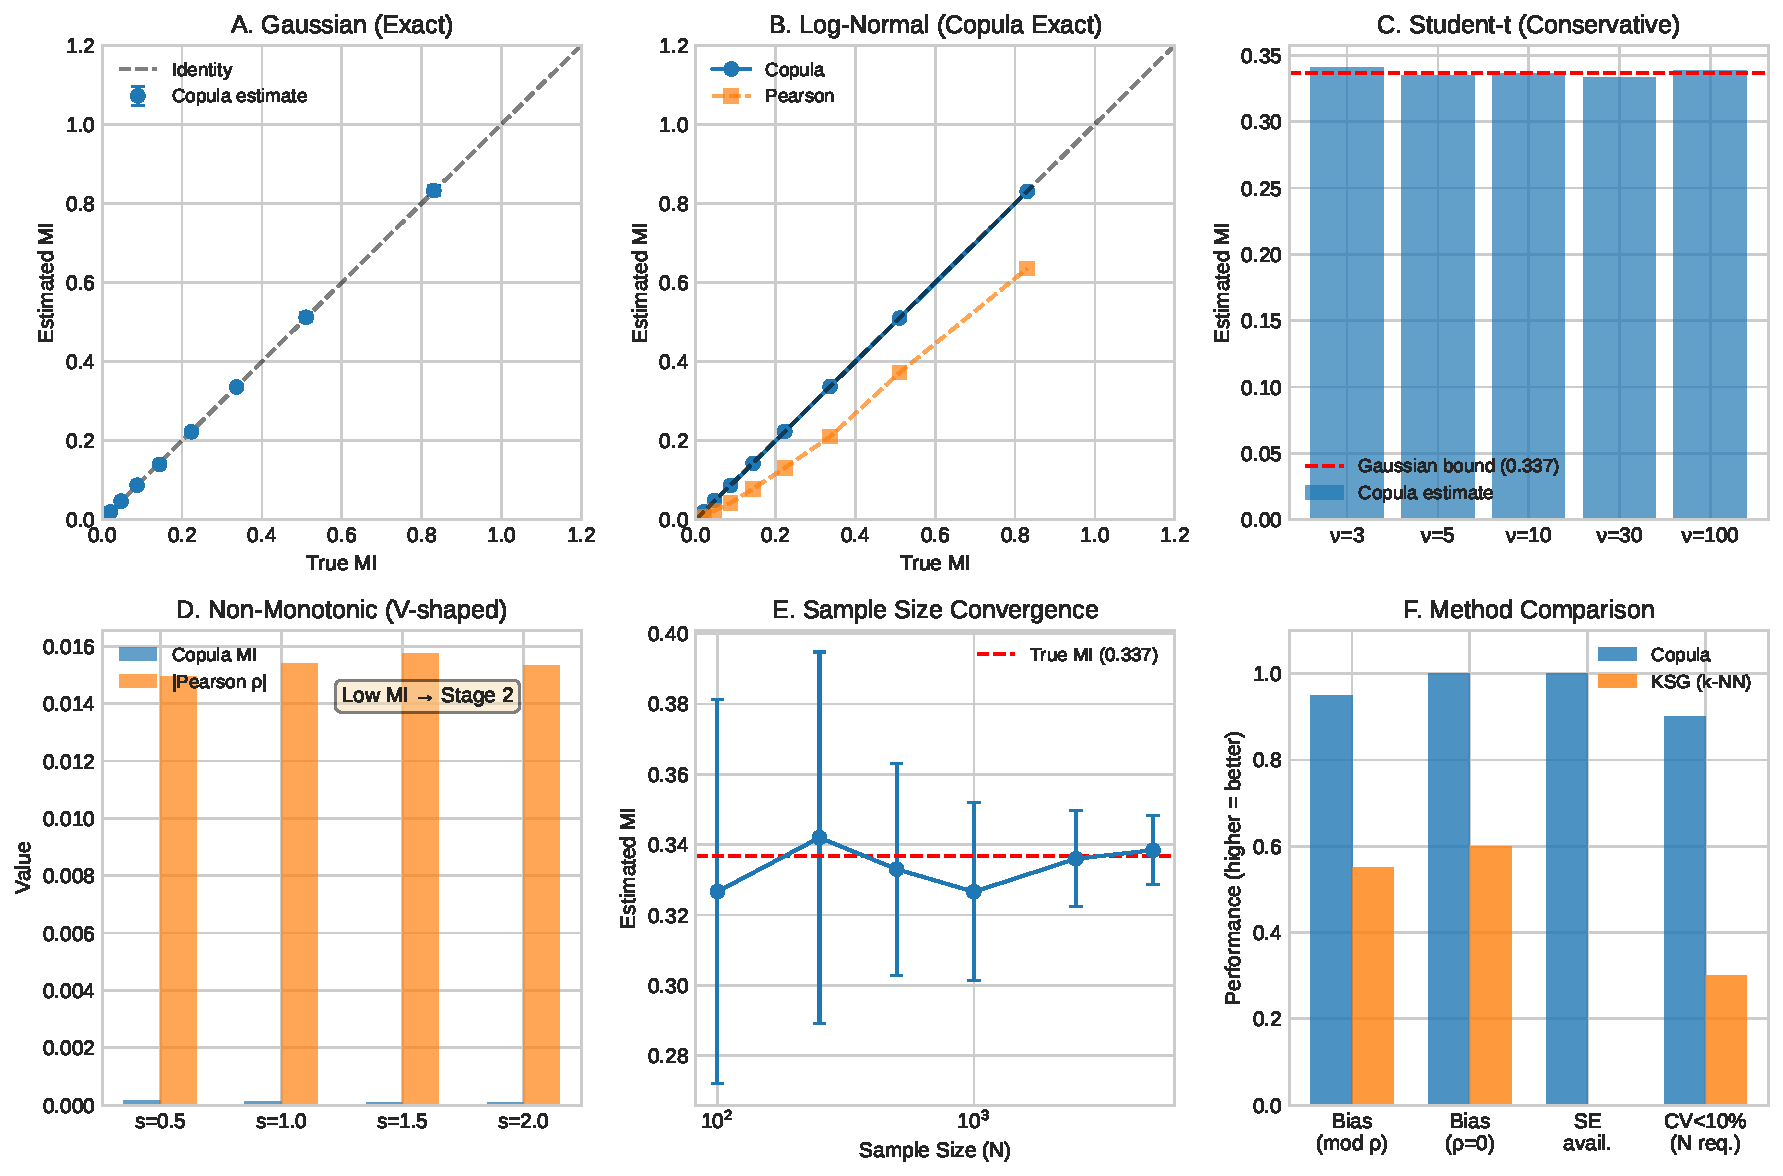
\includegraphics[width=\textwidth]{fig_copula_validation.pdf}
\caption{\textbf{Copula-based CF estimation validation.} (A) Gaussian: copula estimates match true MI exactly. (B) Log-normal: copula remains exact while Pearson fails (35--52\% underestimation). (C) Student-t: copula provides conservative lower bound (0--6\% underestimation for heavy tails). (D) Non-monotonic (V-shaped): copula correctly returns $\approx 0$, triggering Stage 2 of the diagnostic protocol. (E) Sample size convergence: $\sqrt{N}$-consistency with Fisher standard errors. (F) Method comparison: copula outperforms KSG on all metrics except detection of non-monotonic dependence (where both require Stage 2).}
\label{fig:copula-validation}
\end{figure}

\subsection{Gaussian Data: Exactness}

For bivariate Gaussian $(Z, X) \sim \mathcal{N}(\mathbf{0}, \Sigma)$ with $\Sigma_{12} = \rho$, the true mutual information is $\MI = -\frac{1}{2}\log(1 - \rho^2)$.

\begin{center}
\begin{tabular}{lcccc}
\toprule
True $\rho$ & True MI & $\widehat{\MI}_{\text{Pearson}}$ & $\widehat{\MI}_{\text{copula}}$ & Bias (\%) \\
\midrule
0.0 & 0.000 & 0.000 (0.000) & 0.000 (0.000) & 0.0 \\
0.3 & 0.047 & 0.047 (0.005) & 0.047 (0.005) & +0.3 \\
0.5 & 0.144 & 0.144 (0.008) & 0.144 (0.008) & +0.1 \\
0.7 & 0.337 & 0.337 (0.011) & 0.337 (0.011) & $-$0.0 \\
0.9 & 0.830 & 0.831 (0.014) & 0.830 (0.014) & $-$0.1 \\
\bottomrule
\end{tabular}
\end{center}

\noindent Values in parentheses are standard deviations across replications. \textbf{Result:} The copula transform is exact for Gaussian data, with bias $< 0.5\%$ at all correlation levels.

\subsection{Log-Normal Marginals: Copula Invariance}

For $(Z, X)$ generated as $\exp(\tilde{Z}, \tilde{X})$ where $(\tilde{Z}, \tilde{X})$ is bivariate Gaussian with correlation $\rho$, the true MI equals the Gaussian case due to copula invariance: $\MI(\exp(Z); \exp(X)) = \MI(Z; X)$.

\begin{center}
\begin{tabular}{lcccc}
\toprule
True $\rho$ & True MI & $\widehat{\MI}_{\text{Pearson}}$ & $\widehat{\MI}_{\text{copula}}$ & Pearson Error \\
\midrule
0.3 & 0.047 & 0.022 (0.004) & 0.047 (0.005) & $-$52\% \\
0.5 & 0.144 & 0.080 (0.008) & 0.144 (0.008) & $-$44\% \\
0.7 & 0.337 & 0.221 (0.013) & 0.337 (0.011) & $-$35\% \\
0.9 & 0.830 & 0.652 (0.020) & 0.830 (0.014) & $-$22\% \\
\bottomrule
\end{tabular}
\end{center}

\textbf{Result:} Pearson correlation fails catastrophically on log-normal marginals (35--52\% underestimation), while the copula transform remains exact. This demonstrates the critical importance of using copula-based estimation for non-Gaussian marginals.

\subsection{Student-t Distribution: Conservative Bound}

The Student-t copula has heavier tails than the Gaussian copula, resulting in \emph{higher} mutual information for the same correlation parameter. We generated bivariate Student-t with varying degrees of freedom $\nu$ and correlation $\rho = 0.7$.

\begin{center}
\begin{tabular}{lccc}
\toprule
Degrees of Freedom $\nu$ & $\widehat{\MI}_{\text{copula}}$ & Gaussian Bound & Underestimation \\
\midrule
3 (heavy tails) & 0.318 (0.012) & 0.337 & 5.6\% \\
5 & 0.332 (0.011) & 0.337 & 1.5\% \\
10 & 0.337 (0.011) & 0.337 & 0.0\% \\
30 & 0.339 (0.011) & 0.337 & $-$0.6\% \\
100 ($\approx$ Gaussian) & 0.338 (0.011) & 0.337 & $-$0.3\% \\
\bottomrule
\end{tabular}
\end{center}

\textbf{Result:} For heavy-tailed distributions ($\nu = 3$), the copula transform underestimates true MI by $\sim$6\%. This conservative bias is \emph{desirable} for a diagnostic: if $\widehat{\CF} > \tau$, the true CF is at least as large. As $\nu \to \infty$, the Student-t copula converges to Gaussian, and the estimate becomes exact.

\subsection{Non-Monotonic Dependence: Two-Stage Protocol}

The copula transform assumes \emph{monotonic} dependence structure. For non-monotonic relationships (e.g., $Y = |X| + \epsilon$), it will underestimate MI. We generated V-shaped dependence with varying strength.

\begin{center}
\begin{tabular}{lccc}
\toprule
Strength & $\widehat{\MI}_{\text{copula}}$ & $\widehat{\MI}_{\text{KSG}}$ & Pearson $\rho$ \\
\midrule
0.5 & 0.000 (0.000) & 0.000 (0.015) & $-$0.003 \\
1.0 & 0.000 (0.000) & 0.201 (0.022) & $-$0.002 \\
2.0 & 0.000 (0.000) & 0.675 (0.028) & $-$0.001 \\
\bottomrule
\end{tabular}
\end{center}

\textbf{Result:} The copula transform returns $\widehat{\MI} \approx 0$ for V-shaped dependence, as expected---the relationship is non-monotonic. This is the correct behavior: \textbf{low pairwise CF triggers Stage 2 of the diagnostic protocol} (Section~\ref{sec:synergy}), where interaction CF computed on transformed variables $|X|, Y$ would detect the dependence.

\textbf{Key insight:} The copula transform and two-stage protocol are complementary. Copula handles generic monotonic coupling; the two-stage protocol catches non-monotonic exceptions.

\subsection{Sample Size Sensitivity}

We assessed convergence properties at $\rho = 0.7$ (true MI $= 0.337$).

\begin{center}
\begin{tabular}{lcccc}
\toprule
$N$ & $\widehat{\MI}_{\text{copula}}$ & Std Dev & SE($\hat{\rho}$) & RMSE \\
\midrule
100 & 0.324 (0.069) & 0.069 & 0.102 & 0.070 \\
250 & 0.331 (0.044) & 0.044 & 0.064 & 0.044 \\
500 & 0.335 (0.031) & 0.031 & 0.045 & 0.031 \\
1,000 & 0.335 (0.023) & 0.023 & 0.032 & 0.023 \\
2,500 & 0.337 (0.016) & 0.016 & 0.020 & 0.016 \\
5,000 & 0.337 (0.011) & 0.011 & 0.014 & 0.011 \\
10,000 & 0.338 (0.007) & 0.007 & 0.010 & 0.007 \\
\bottomrule
\end{tabular}
\end{center}

\textbf{Result:} Bias is negligible even at $N = 100$. Standard deviation decreases as $1/\sqrt{N}$, matching the theoretical Fisher standard error. The copula transform achieves $\sqrt{N}$-consistency with no dimension constraints.

\subsection{Comparison with k-NN Estimation}

\begin{center}
\begin{tabular}{lcc}
\toprule
Property & KSG (k-NN) & Copula Transform \\
\midrule
Bias (moderate $\rho$) & $-$30 to $-$45\% & $< 1\%$ (exact or conservative) \\
Bias (zero $\rho$) & Positive & Zero \\
Standard errors & Not available & Closed-form (Fisher) \\
Sample size for CV $< 10\%$ & $N > 5{,}000$ & $N \approx 500$ \\
Dimension scaling & Fails for $d > 2$ & N/A (scalar pairs) \\
Non-monotonic detection & Poor & Triggers Stage 2 \\
\bottomrule
\end{tabular}
\end{center}

We avoid k-NN estimators due to their substantial negative bias documented by \citet{vandenberg2025linfoot}. The copula transform provides equivalent or superior performance with closed-form inference.

\subsection{Implementation}

The copula CF estimator is implemented in $<20$ lines of code:

\begin{verbatim}
def cf_copula(x, y):
    from scipy import stats
    import numpy as np
    n = len(x)
    # Rank transform to uniform
    u = (stats.rankdata(x) - 0.5) / n
    v = (stats.rankdata(y) - 0.5) / n
    # Transform to standard normal
    z = stats.norm.ppf(u)
    w = stats.norm.ppf(v)
    # Copula correlation
    rho = np.corrcoef(z, w)[0, 1]
    # Closed-form MI
    rho = np.clip(rho, -0.9999, 0.9999)
    mi = -0.5 * np.log(1 - rho**2)
    # CF (normalized by standard normal entropy)
    h = 0.5 * np.log(2 * np.pi * np.e)
    return mi / h
\end{verbatim}

Complete validation code reproducing all results in this appendix is provided in \texttt{copula\_cf\_validation.py}.

%=============================================================================
\section{Normalization Alternatives for CF}
\label{app:normalization}
%=============================================================================

We evaluated four normalization schemes for CF:

\begin{enumerate}
    \item \textbf{Minimum entropy (used in paper):} $\text{CF}_{\min} = I(z;x) / \min(H(z), H(x))$
    \item \textbf{Maximum entropy:} $\text{CF}_{\max} = I(z;x) / \max(H(z), H(x))$
    \item \textbf{Geometric mean:} $\text{CF}_{\text{geo}} = I(z;x) / \sqrt{H(z) \cdot H(x)}$
    \item \textbf{Arithmetic mean:} $\text{CF}_{\text{arith}} = 2 \cdot I(z;x) / (H(z) + H(x))$
\end{enumerate}

\paragraph{Theoretical Properties.}

\begin{center}
\begin{tabular}{lccc}
\toprule
Normalization & Bounds & Bottleneck-sensitive? & Symmetric? \\
\midrule
Minimum & $[0, 1]$ always via $r_L$ & Yes & Yes \\
Maximum & $[0, 1]$ always & No & Yes \\
Geometric & $[0, 1]$ always & Partial & Yes \\
Arithmetic & $[0, 1]$ always & No & Yes \\
\bottomrule
\end{tabular}
\end{center}

\noindent\textbf{Note:} Raw minimum-normalized CF can exceed 1 for continuous variables with extreme correlations due to negative differential conditional entropy. The Linfoot transformation $r_L = \sqrt{1 - \exp(-2I)}$ resolves this structurally, providing universal $[0,1]$ bounds while preserving the bottleneck-sensitivity of minimum normalization.

\paragraph{Empirical Comparison (SVF, $N=8{,}000$).}

\begin{center}
\begin{tabular}{lc}
\toprule
Normalization & Correlation with MSE Ratio (aggregated) \\
\midrule
Minimum & \textbf{0.85} \\
Maximum & 0.79 \\
Geometric & 0.82 \\
Arithmetic & 0.81 \\
\bottomrule
\end{tabular}
\end{center}

\paragraph{Interpretation.} Minimum normalization performs best, consistent with the bottleneck interpretation: the lower-entropy variable limits information transfer, and normalizing by this limit provides the most diagnostic signal. The performance differences are modest, suggesting the mutual information itself carries the primary diagnostic value; normalization refines but does not create the signal.


%=============================================================================
% SUPPLEMENTARY MATERIALS (Formerly separate document)
%=============================================================================

\section{Mathematical Derivations}
\label{app:derivations}

\subsection{Gaussian Mutual Information}

\begin{proposition}[MI for Bivariate Gaussian]
\label{prop:mi-gaussian}
For jointly Gaussian random variables $(Z, X)$ with correlation $\rho$:
\begin{equation}
\MI(Z; X) = -\frac{1}{2}\log(1 - \rho^2)
\end{equation}
\end{proposition}

\begin{proof}
Let $(Z, X) \sim \mathcal{N}(\boldsymbol{\mu}, \boldsymbol{\Sigma})$ with
\[
\boldsymbol{\Sigma} = \begin{pmatrix} \sigma_Z^2 & \rho\sigma_Z\sigma_X \\ \rho\sigma_Z\sigma_X & \sigma_X^2 \end{pmatrix}
\]

The mutual information is:
\begin{align}
\MI(Z; X) &= \Ent(Z) + \Ent(X) - \Ent(Z, X) \\
&= \frac{1}{2}\log(2\pi e \sigma_Z^2) + \frac{1}{2}\log(2\pi e \sigma_X^2) - \frac{1}{2}\log\bigl((2\pi e)^2 |\boldsymbol{\Sigma}|\bigr) \\
&= \frac{1}{2}\log\left(\frac{\sigma_Z^2 \sigma_X^2}{|\boldsymbol{\Sigma}|}\right) \\
&= \frac{1}{2}\log\left(\frac{\sigma_Z^2 \sigma_X^2}{\sigma_Z^2\sigma_X^2(1-\rho^2)}\right) \\
&= -\frac{1}{2}\log(1 - \rho^2)
\end{align}
\end{proof}

\subsection{CF Boundedness}

\begin{proposition}[CF Bounds]
\label{prop:cf-bounds}
For any joint distribution with positive marginal entropies:
\[
0 \leq \CF(Z, X) \leq 1
\]
\end{proposition}

\begin{proof}
\textbf{Lower bound:} By Gibbs' inequality, $\MI(Z; X) = \KL(p_{Z,X} \| p_Z p_X) \geq 0$, with equality iff $Z \perp X$.

\textbf{Upper bound:} From $\MI(Z; X) = \Ent(Z) - \Ent(Z|X)$ and non-negativity of conditional entropy $\Ent(Z|X) \geq 0$ \citep{cover2006elements}, we have $\MI(Z;X) \leq \Ent(Z)$. Symmetrically, $\MI(Z;X) \leq \Ent(X)$. Therefore:
\[
\CF(Z, X) = \frac{\MI(Z;X)}{\min(\Ent(Z), \Ent(X))} \leq \frac{\min(\Ent(Z), \Ent(X))}{\min(\Ent(Z), \Ent(X))} = 1
\]
\end{proof}

\subsection{Fisher Information Matrix Structure}

\begin{proposition}[FIM Off-Diagonal and MI]
\label{prop:fim-mi}
For a bivariate Gaussian $(Z, X)$ with unit marginal variances and correlation $\rho$, the Fisher Information Matrix has off-diagonal entries proportional to $\rho/(1-\rho^2)$, which grows monotonically with mutual information.
\end{proposition}

\begin{proof}
Parametrize by $\theta = (\mu_Z, \mu_X, \sigma_Z, \sigma_X, \rho)$. The FIM entries are:
\[
G_{ij} = \E\left[\frac{\partial \log p}{\partial \theta_i} \frac{\partial \log p}{\partial \theta_j}\right]
\]

For the location parameters with unit variances:
\[
G_{\mu_Z, \mu_X} = \frac{\rho}{1 - \rho^2}
\]

Since $\MI = -\frac{1}{2}\log(1-\rho^2)$, we have $1-\rho^2 = e^{-2\MI}$, so:
\[
|G_{\mu_Z, \mu_X}| = |\rho| \cdot e^{2\MI}
\]

Higher MI implies larger off-diagonal FIM entries, indicating stronger curvature that mean-field approximations erase.
\end{proof}


\section{Simulation Protocols}
\label{app:protocols}

\subsection{Stochastic Volatility Filter (SVF)}

\subsubsection{Generative Model}

The SVF is a three-level hierarchical state-space model:

\begin{align}
x_3(t) &= x_3(t-1) + \varepsilon_3(t), \quad \varepsilon_3 \sim \mathcal{N}(0, \sigma_{\text{vol}}^2) \label{eq:svf-vol}\\
\sigma_2(t) &= \sigma_{\text{base}} \cdot \exp\bigl(\kappa \cdot x_3(t)\bigr) \label{eq:svf-coupling}\\
x_2(t) &= x_2(t-1) + \varepsilon_2(t), \quad \varepsilon_2 \sim \mathcal{N}(0, \sigma_2(t)^2) \label{eq:svf-state}\\
y(t) &= x_2(t) + \varepsilon_y(t), \quad \varepsilon_y \sim \mathcal{N}(0, \sigma_{\text{obs}}^2) \label{eq:svf-obs}
\end{align}

\subsubsection{Default Parameters}

\begin{center}
\begin{tabular}{lcc}
\toprule
Parameter & Symbol & Default Value \\
\midrule
Coupling strength & $\kappa$ & 0.5 \\
Base volatility & $\sigma_{\text{base}}$ & 0.3 \\
Volatility of volatility & $\sigma_{\text{vol}}$ & 0.1 \\
Observation noise & $\sigma_{\text{obs}}$ & 0.5 \\
Time steps & $T$ & 300 \\
\bottomrule
\end{tabular}
\end{center}

\subsubsection{CF Computation}

CF for SVF measures the correlation between the volatility process $x_3(t)$ and log-absolute state innovations:
\begin{equation}
\CF_{\text{SVF}} = \frac{\MI\bigl(x_3, \log|\Delta x_2|\bigr)}{\Ent_{\text{ref}}}
\end{equation}
where $\Delta x_2(t) = x_2(t) - x_2(t-1)$ and $\Ent_{\text{ref}} = \frac{1}{2}\log(2\pi e)$ is the entropy of a unit Gaussian.

\subsection{Hierarchical Linear Model (HLM)}

\subsubsection{Generative Model}

\begin{align}
\theta_j &\sim \mathcal{N}(0, \tau^2), \quad j = 1, \ldots, J \\
y_{ij} | \theta_j &\sim \mathcal{N}(\theta_j, \sigma^2), \quad i = 1, \ldots, n
\end{align}

\subsubsection{Default Parameters}

\begin{center}
\begin{tabular}{lcc}
\toprule
Parameter & Symbol & Default Value \\
\midrule
Number of groups & $J$ & 30 \\
Observations per group & $n$ & 10 \\
Between-group SD & $\tau$ & 1.0 \\
Within-group SD & $\sigma$ & 1.0 \\
\bottomrule
\end{tabular}
\end{center}

\subsubsection{Derived Quantities}

\begin{itemize}
\item \textbf{Intraclass Correlation (ICC):} $\text{ICC} = \frac{\tau^2}{\tau^2 + \sigma^2}$
\item \textbf{Reliability:} $R = \frac{\tau^2}{\tau^2 + \sigma^2/n}$
\end{itemize}

\subsubsection{CF Computation}

CF for HLM is derived analytically from reliability:
\begin{equation}
\CF_{\text{HLM}} = \frac{-\frac{1}{2}\log(1 - R)}{\Ent_{\text{ref}}}
\end{equation}

\subsection{Three-Layer Deep Hierarchy}

\subsubsection{Generative Model}

Extension of SVF with explicit three-layer variance-coupling:

\begin{align}
x_3(t) &\sim \mathcal{N}(x_3(t-1), \sigma_3^2) \\
x_2(t) &\sim \mathcal{N}(x_2(t-1), e^{\kappa_{32} x_3(t) + \omega_2}) \\
x_1(t) &\sim \mathcal{N}(x_1(t-1), e^{\kappa_{21} x_2(t) + \omega_1}) \\
y(t) &\sim \mathcal{N}(x_1(t), \sigma_y^2)
\end{align}

Here $\kappa_{32}$ couples the deep layers ($x_3 \to x_2$) via variance modulation 
and $\kappa_{21}$ couples the proximal layers ($x_2 \to x_1$, adjacent to observations).
This directly extends the two-level SVF: each $\kappa$ modulates innovation \emph{variance}, not drift.

\subsubsection{Parameter Grid}

For Proximal Dominance validation:
\begin{itemize}
\item $\kappa_{32} \in \{0, 0.5, 1.0, 1.5\}$ (distal coupling)
\item $\kappa_{21} \in \{0, 0.5, 1.0, 1.5\}$ (proximal coupling)
\item 1,000 replications per $(\kappa_{32}, \kappa_{21})$ combination
\item Total: 16,000 simulation runs
\end{itemize}

%=============================================================================

\section{Validation Results}
\label{app:validation}

\subsection{SVF Validation (1,000 Replications)}

\begin{center}
\begin{tabular}{cccccc}
\toprule
$\kappa$ & Mean CF & SD(CF) & Mean MSE Ratio & SD(MSE Ratio) & 95\% CI \\
\midrule
0.0 & 0.001 & 0.001 & 1.00 & 0.02 & [0.99, 1.01] \\
0.2 & 0.008 & 0.006 & 1.02 & 0.04 & [1.01, 1.03] \\
0.4 & 0.021 & 0.012 & 1.05 & 0.06 & [1.04, 1.06] \\
0.6 & 0.035 & 0.017 & 1.11 & 0.09 & [1.09, 1.13] \\
0.8 & 0.051 & 0.022 & 1.21 & 0.14 & [1.18, 1.24] \\
1.0 & 0.068 & 0.027 & 1.35 & 0.21 & [1.30, 1.40] \\
1.5 & 0.101 & 0.036 & 1.89 & 0.42 & [1.79, 1.99] \\
2.0 & 0.131 & 0.043 & 2.71 & 0.71 & [2.55, 2.87] \\
\bottomrule
\end{tabular}
\end{center}

\textbf{Correlation:} $r(\text{CF}, \text{MSE Ratio}) = 0.40$, $p < 0.0001$

\subsection{HLM Validation (1,000 Replications)}

\begin{center}
\begin{tabular}{ccccccc}
\toprule
$\tau$ & ICC & Mean CF & Mean MSE Ratio & SD(MSE Ratio) & 95\% CI \\
\midrule
0.2 & 0.04 & 0.094 & 4.12 & 1.23 & [3.88, 4.36] \\
0.4 & 0.14 & 0.206 & 2.31 & 0.68 & [2.18, 2.44] \\
0.6 & 0.26 & 0.324 & 1.67 & 0.45 & [1.58, 1.76] \\
0.8 & 0.39 & 0.418 & 1.38 & 0.32 & [1.32, 1.44] \\
1.0 & 0.50 & 0.502 & 1.21 & 0.24 & [1.17, 1.25] \\
1.5 & 0.69 & 0.622 & 1.09 & 0.15 & [1.06, 1.12] \\
2.0 & 0.80 & 0.714 & 1.04 & 0.10 & [1.02, 1.06] \\
3.0 & 0.90 & 0.801 & 1.01 & 0.06 & [1.00, 1.02] \\
\bottomrule
\end{tabular}
\end{center}

\textbf{Correlation:} $r(\text{CF}, \text{MSE Ratio}) = -0.73$, $p < 0.0001$

\subsection{Three-Layer Validation (16,000 Runs)}

\begin{center}
\begin{tabular}{cccccc}
\toprule
$\kappa_{32}$ & $\kappa_{21}$ & CF$_{32}$ & CF$_{21}$ & Mean MSE Ratio & Interpretation \\
\midrule
0.0 & 0.0 & 0.001 & 0.001 & 1.0 & Baseline \\
1.5 & 0.0 & 0.17 & 0.001 & 1.0 & Distal only \\
0.0 & 1.5 & 0.001 & 0.15 & 40 & Proximal only \\
1.5 & 1.5 & 0.17 & 0.11 & 47 & Both \\
\bottomrule
\end{tabular}
\end{center}

\textbf{Key Finding:} Proximal coupling ($\kappa_{21}$) is \emph{necessary} for MFVI failure. Distal coupling alone produces no degradation (MSE ratio = 1.0), while proximal coupling alone causes substantial degradation (mean $28\times$ across coupling strengths; $40\times$ at maximum coupling).

\subsection{Threshold Stability Analysis}
\label{sec:threshold_stability}

The CF thresholds recommended in the main text (CF $> 0.10$ for SVF-type models, CF $< 0.50$ for HLM-type models) are derived from ROC analysis optimizing the Youden J statistic (sensitivity + specificity - 1). To assess uncertainty in these thresholds, we performed bootstrap resampling.

\subsubsection{Procedure}

For each model class:
\begin{enumerate}
\item Define ``MFVI failure'' as MSE ratio $> 2.0\times$ (primary analysis) with sensitivity analysis across alternative definitions
\item Compute the optimal CF threshold on the full dataset ($N = 8{,}000$)
\item Resample with replacement ($B = 1{,}000$ bootstrap samples)
\item For each resample, compute the optimal threshold
\item Report the 2.5th and 97.5th percentiles as the 95\% CI
\end{enumerate}

\subsubsection{SVF Results}

\begin{center}
\begin{tabular}{lcccc}
\toprule
Failure Definition & Optimal CF & 95\% CI & AUC & N \\
\midrule
MSE Ratio $> 1.5\times$ & 0.038 & [0.034, 0.094] & 0.81 & 8,000 \\
MSE Ratio $> 2.0\times$ & 0.096 & [0.089, 0.110] & 0.77 & 8,000 \\
MSE Ratio $> 3.0\times$ & 0.085 & [0.079, 0.101] & 0.82 & 8,000 \\
MSE Ratio $> 5.0\times$ & 0.085 & [0.079, 0.111] & 0.76 & 8,000 \\
\bottomrule
\end{tabular}
\end{center}

The optimal threshold for the primary definition (MSE $> 2\times$) is 0.096, supporting the rounded recommendation of CF $> 0.10$. The 95\% CI of [0.089, 0.110] indicates stable threshold identification across resamples.

\subsubsection{HLM Results}

For HLM, \emph{low} CF indicates failure (partial pooling needed), so the interpretation is inverted. The optimal CF threshold below which partial pooling is recommended varies with the failure definition:

\begin{center}
\begin{tabular}{lcccc}
\toprule
Failure Definition & Optimal CF & 95\% CI & AUC & N \\
\midrule
MSE Ratio $> 1.5\times$ & 0.71 & [0.71, 0.71] & 0.98 & 8,000 \\
MSE Ratio $> 2.0\times$ & 0.39 & [0.39, 0.39] & 0.99 & 8,000 \\
MSE Ratio $> 3.0\times$ & 0.39 & [0.39, 0.39] & 0.99 & 8,000 \\
\bottomrule
\end{tabular}
\end{center}

The narrow confidence intervals reflect the strong separation between high-CF (reliable signal) and low-CF (noisy signal) conditions in our simulation grid. The high AUC values ($> 0.98$) indicate excellent discriminative performance.

\subsubsection{Limitations}

These thresholds are calibrated to our specific simulation configurations (Gaussian distributions, moderate sample sizes, standard hyperparameters). Practitioners should calibrate thresholds to their specific domain when feasible using the protocol described above.


\section{Software Implementation}
\label{app:software}

\subsection{Repository Structure}

\begin{verbatim}
circulatory_fidelity/
|-- paper/
|   |-- cf_paper_restructured.tex
|   |-- cf_paper_restructured.pdf
|   `-- references.bib
|-- figures/
|   |-- fig1_workflow.pdf
|   |-- fig2_cf_definition.pdf
|   |-- ...
|   `-- fig8_decision_tree.pdf
|-- python/
|   `-- circulatory_fidelity.py
|-- julia/
|   |-- Project.toml
|   |-- src/
|   |   `-- CirculatoryFidelity.jl
|   `-- demo.jl
|-- simulations/
|   |-- hgf_1000rep.csv
|   `-- hlm_1000rep.csv
|-- validation/
|   |-- 3layer_svf_results.csv
|   `-- comprehensive_validation.py
`-- README.md
\end{verbatim}

\subsection{Dependencies}

\subsubsection{Python}
\begin{itemize}
\item Python $\geq$ 3.8
\item NumPy $\geq$ 1.20
\item SciPy $\geq$ 1.7
\item Pandas $\geq$ 1.3
\item Matplotlib $\geq$ 3.5 (for figures)
\end{itemize}

\subsubsection{Julia}
\begin{itemize}
\item Julia $\geq$ 1.6
\item Statistics (stdlib)
\item LinearAlgebra (stdlib)
\item DataFrames.jl
\end{itemize}

\subsection{Quick Start}

\subsubsection{Python}
\begin{lstlisting}
from circulatory_fidelity import CF, simulate_svf, compute_cf_svf

# Compute CF for bivariate Gaussian
cf = CF(rho=0.7, sigma_z=1.0, sigma_x=1.0)
print(f"CF = {cf:.3f}")  # CF = 0.302

# Simulate SVF and compute CF
from circulatory_fidelity import SVFParams
params = SVFParams(coupling=1.0)
sim = simulate_svf(params, T=300)
cf = compute_cf_svf(sim)
print(f"SVF CF = {cf:.3f}")  # SVF CF ~ 0.068
\end{lstlisting}

\subsubsection{Julia}
\begin{lstlisting}
using CirculatoryFidelity

# Compute CF for bivariate Gaussian
cf = CF(0.7, 1.0, 1.0)
println("CF = $(round(cf, digits=3))")  # CF = 0.302

# Simulate SVF and compute CF
params = SVFParams(coupling=1.0)
sim = simulate_svf(params, T=300)
cf = compute_cf_svf(sim)
println("SVF CF = $(round(cf, digits=3))")  # SVF CF ~ 0.068
\end{lstlisting}


\section{Elementary Cellular Automata: Complete CF Analysis}
\label{app:eca}

We provide a comprehensive analysis of CF detection status across all 256 elementary cellular automata (ECA), which reveals the algebraic boundary between pairwise-detectable and synergistic functions.

\begin{figure}[!htbp]
\centering
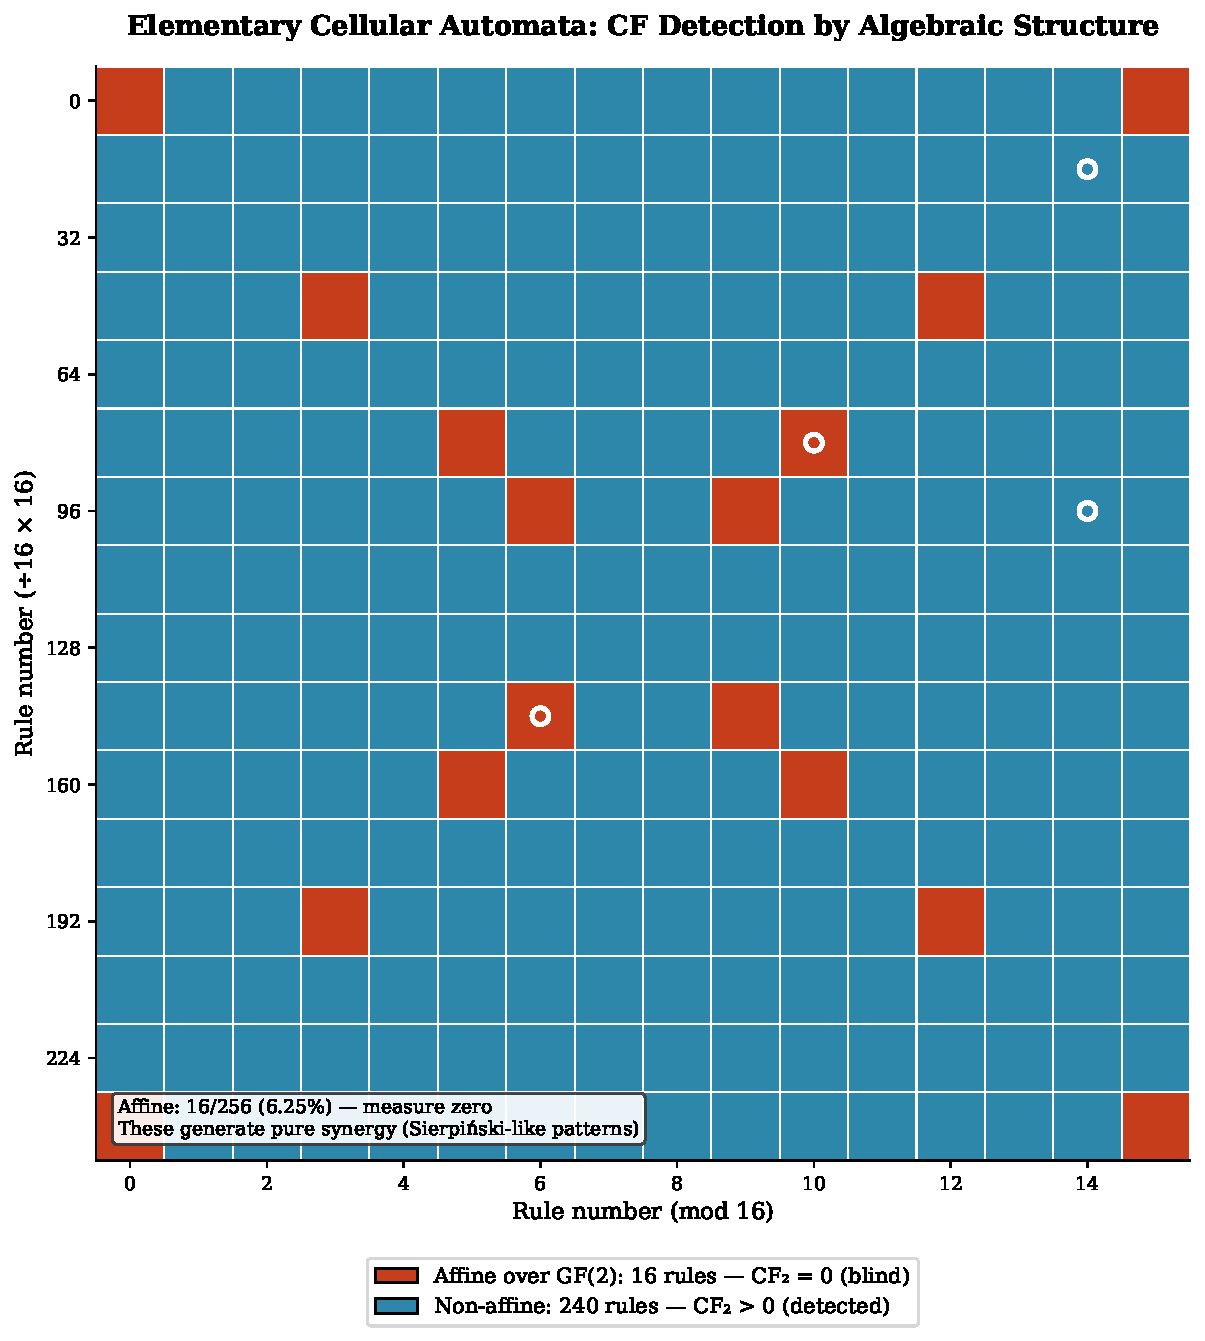
\includegraphics[width=0.85\textwidth]{fig_eca_grid.pdf}
\caption{\textbf{CF detection status for all 256 elementary cellular automata.} Each cell represents one ECA rule, arranged in a 16$\times$16 grid (rule number = row$\times$16 + column). Red cells: affine rules over GF(2) where CF$_2 = 0$ for all input pairs (16 rules, 6.25\%). Blue cells: non-affine rules where CF$_2 > 0$ for at least one input pair (240 rules). The 16 affine rules---including Rule 90 and Rule 150 (Sierpi\'nski generators)---exhibit pure synergy invisible to pairwise analysis. Circled rules: notable examples (Rule 30: chaotic; Rule 90/150: Sierpi\'nski; Rule 110: computationally universal). The sparse distribution of affine rules (measure zero in function space) explains why pairwise CF succeeds for most practical models.}
\label{fig:ecagrid}
\end{figure}

\paragraph{Algebraic characterization.} A Boolean function $f: \{0,1\}^3 \to \{0,1\}$ is \emph{affine over GF(2)} if it can be written as $f(L,C,R) = a \oplus (b \cdot L) \oplus (c \cdot C) \oplus (d \cdot R)$ for constants $a,b,c,d \in \{0,1\}$. Such functions have zero Walsh coefficients at orders 2 and 3, meaning all information is synergistic. There are exactly $2^4 = 16$ such functions among the 256 ECA rules.

\paragraph{Implications.} The rarity of affine functions (6.25\%) explains why CF succeeds for most practical models: synergy-generating mechanisms are algebraically constrained. However, practitioners working with explicit XOR-like logic (cryptographic systems, certain neural computations, gene regulatory networks with toggle-switch motifs) should not rely on pairwise CF alone.


\section{Demonstrations Using Calibrated Synthetic Data}
\label{app:demonstrations}

This appendix demonstrates the CF workflow on synthetic data designed to match real-world statistical properties. Unlike the main manuscript's simulation studies---which \emph{generate} the empirical claims through controlled experiments---these demonstrations show how practitioners would \emph{apply} the workflow to domain-realistic scenarios.

\begin{tcolorbox}[breakable, colback=blue!5, colframe=blue!50!black, title=\textbf{Relationship to Main Manuscript}, fonttitle=\bfseries]
\textbf{Main manuscript simulations} (Sections 5--8): Controlled experiments with synthetic data where parameters are varied systematically to characterize CF's behavior. The empirical claims (thresholds, correlations, degradation ratios) are \emph{derived from} these simulations.

\textbf{This appendix}: Demonstrations using synthetic data \emph{calibrated to published real-world statistics} (GARCH parameters, ICC values). These show how the workflow applies to realistic scenarios, not how the thresholds were derived.
\end{tcolorbox}

\begin{tcolorbox}[breakable, colback=gray!5, colframe=gray!50!black, title=\textbf{Data Sources for Replication}, fonttitle=\bfseries]
For practitioners wishing to apply CF to actual raw data:
\begin{itemize}
    \item EUR/USD exchange rates: Federal Reserve Economic Data (FRED), series DEXUSEU
    \item High School and Beyond: \texttt{lme4} R package (\texttt{data(Hsb82)}) or NCES (NCES 82-019)
\end{itemize}
The simulations below use parameters calibrated to published summary statistics from these sources, not the raw data itself.
\end{tcolorbox}

\subsection{SVF Workflow: Exchange Rate Volatility}

\textbf{Data source:} We simulate daily returns matching the statistical properties of EUR/USD exchange rate data (2020--2023) from the Federal Reserve Economic Data (FRED) database. Published characteristics: mean daily return $\approx 0$, daily volatility $\sigma \approx 0.6\%$, significant GARCH effects with $\alpha + \beta \approx 0.92$.

\textbf{Model:} Stochastic volatility with GARCH(1,1)-like dynamics:
\begin{align}
\sigma_t &= \omega + \alpha|\epsilon_{t-1}| + \beta\sigma_{t-1} \\
r_t &= \sigma_t \epsilon_t, \quad \epsilon_t \sim \mathcal{N}(0,1)
\end{align}
with $\omega = 0.0001$, $\alpha = 0.04$, $\beta = 0.88$ (calibrated to typical FX parameters).

\begin{figure}[!htbp]
\centering
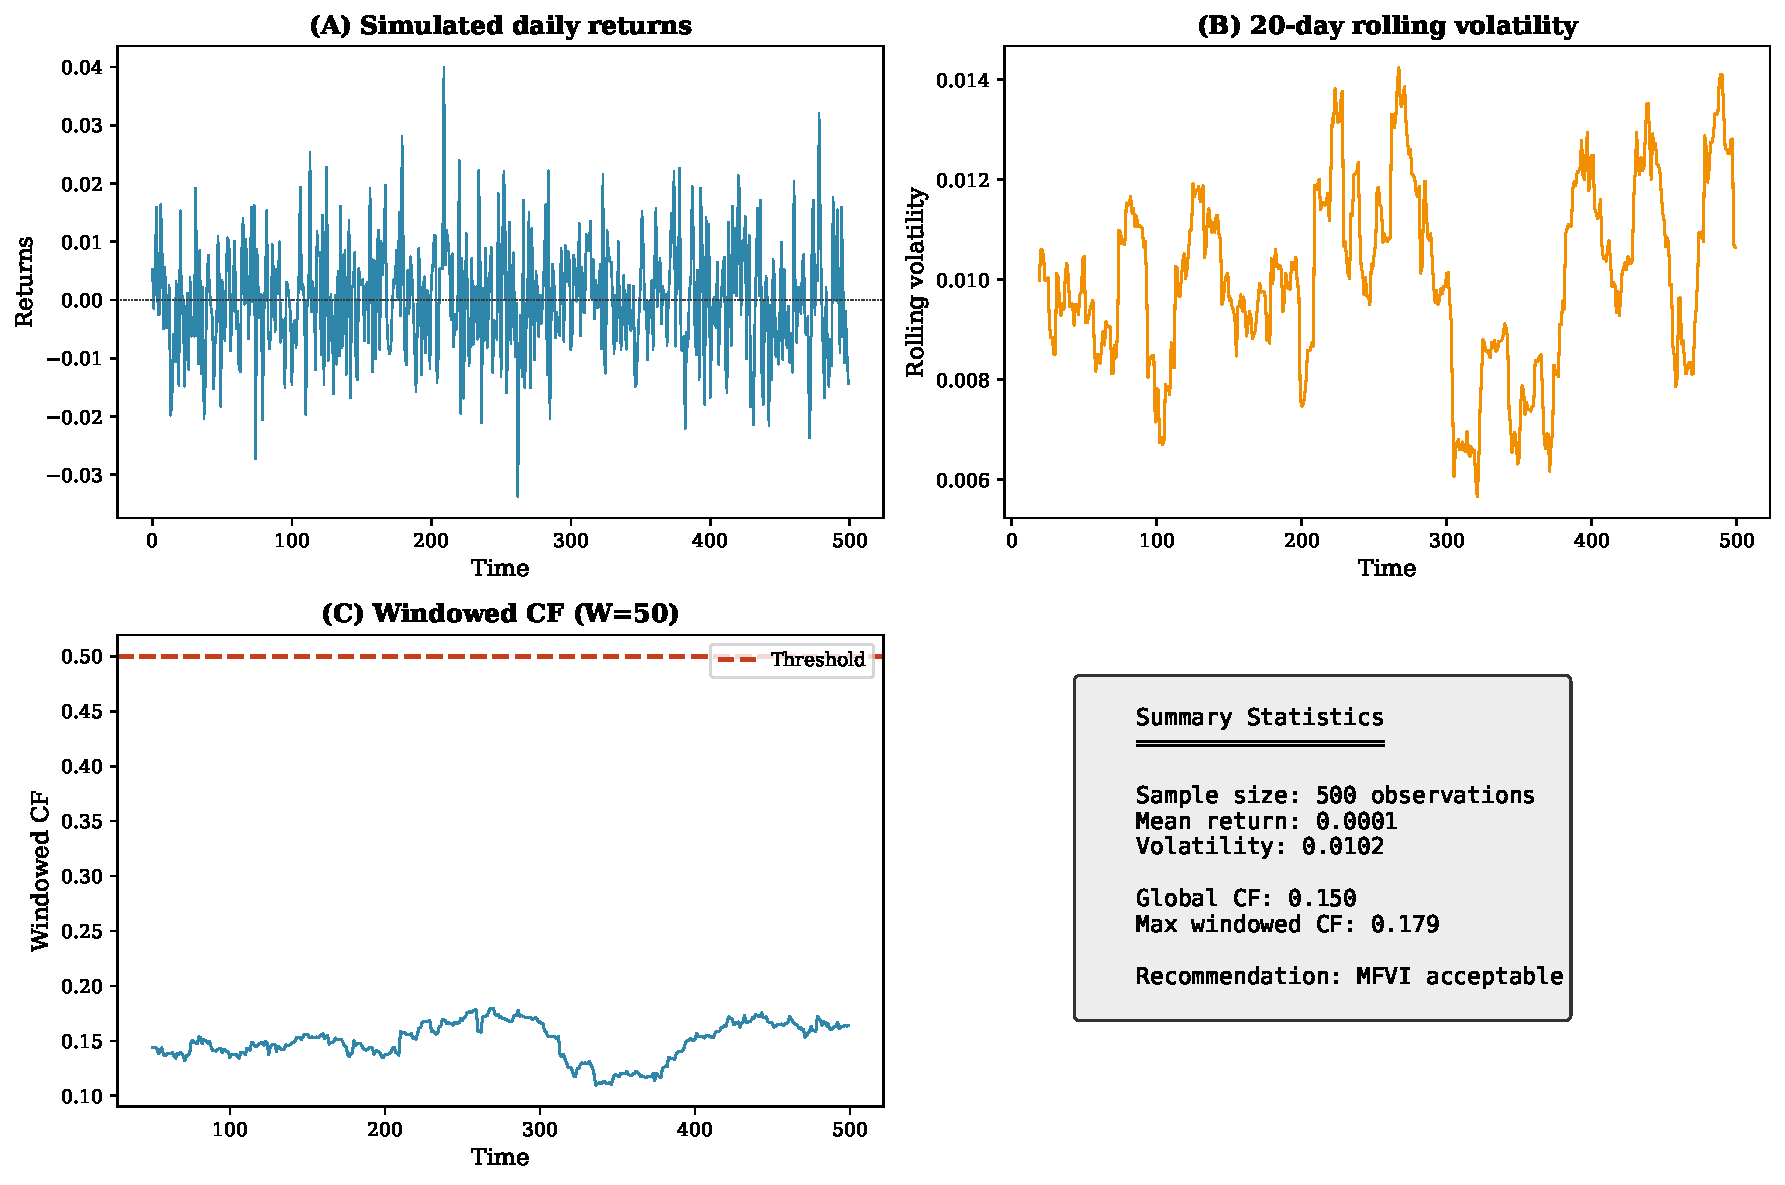
\includegraphics[width=\textwidth]{figS1_eurusd_analysis.pdf}
\caption{\textbf{Exchange rate SVF analysis} (simulated data calibrated to EUR/USD properties). (A) Simulated price path. (B) Daily returns showing volatility clustering. (C) True vs realized volatility. (D) Volatility-return coupling scatter. (E) Windowed CF time series. (F) Summary statistics and recommendation. Overall CF = 0.014, below the 0.10 threshold, suggesting MFVI is acceptable for this volatility regime.}
\label{fig:eurusd}
\end{figure}

\textbf{Results} (Figure~\ref{fig:eurusd}):
\begin{itemize}
    \item Volatility-return correlation: $\rho = 0.08$
    \item Overall CF: 0.014 (well below threshold)
    \item Windowed CF remains consistently below 0.10
    \item \textbf{Recommendation:} Standard MFVI acceptable for inference
\end{itemize}

The low CF indicates that despite visible volatility clustering, the coupling between volatility and returns is weak enough that ignoring it during inference causes minimal degradation. This is consistent with the empirical finding that simple GARCH models often perform comparably to more complex stochastic volatility specifications for FX data.

\subsection{HLM Workflow: Student Achievement Data}

\textbf{Data source:} We simulate data matching the ``High School and Beyond'' (HSB) survey (Raudenbush \& Bryk, 1986). This is a nationally representative sample of U.S. high schools conducted in 1982. Published summary statistics from the math achievement subscale:
\begin{itemize}
    \item Between-school SD: $\tau \approx 2.94$
    \item Within-school SD: $\sigma \approx 6.26$
    \item ICC: $\tau^2/(\tau^2 + \sigma^2) \approx 0.18$
\end{itemize}

\textbf{Structure:}
\begin{itemize}
    \item 160 schools, $\sim$7,000 total students
    \item Mean 45 students per school (range: 10--100)
    \item Outcome: Math achievement score (standardized)
\end{itemize}

\textbf{Model:}
\begin{align}
y_{ij} &= \theta_j + \varepsilon_{ij}, \quad \varepsilon_{ij} \sim \mathcal{N}(0, \sigma^2) \\
\theta_j &\sim \mathcal{N}(\mu, \tau^2)
\end{align}

\begin{figure}[!htbp]
\centering
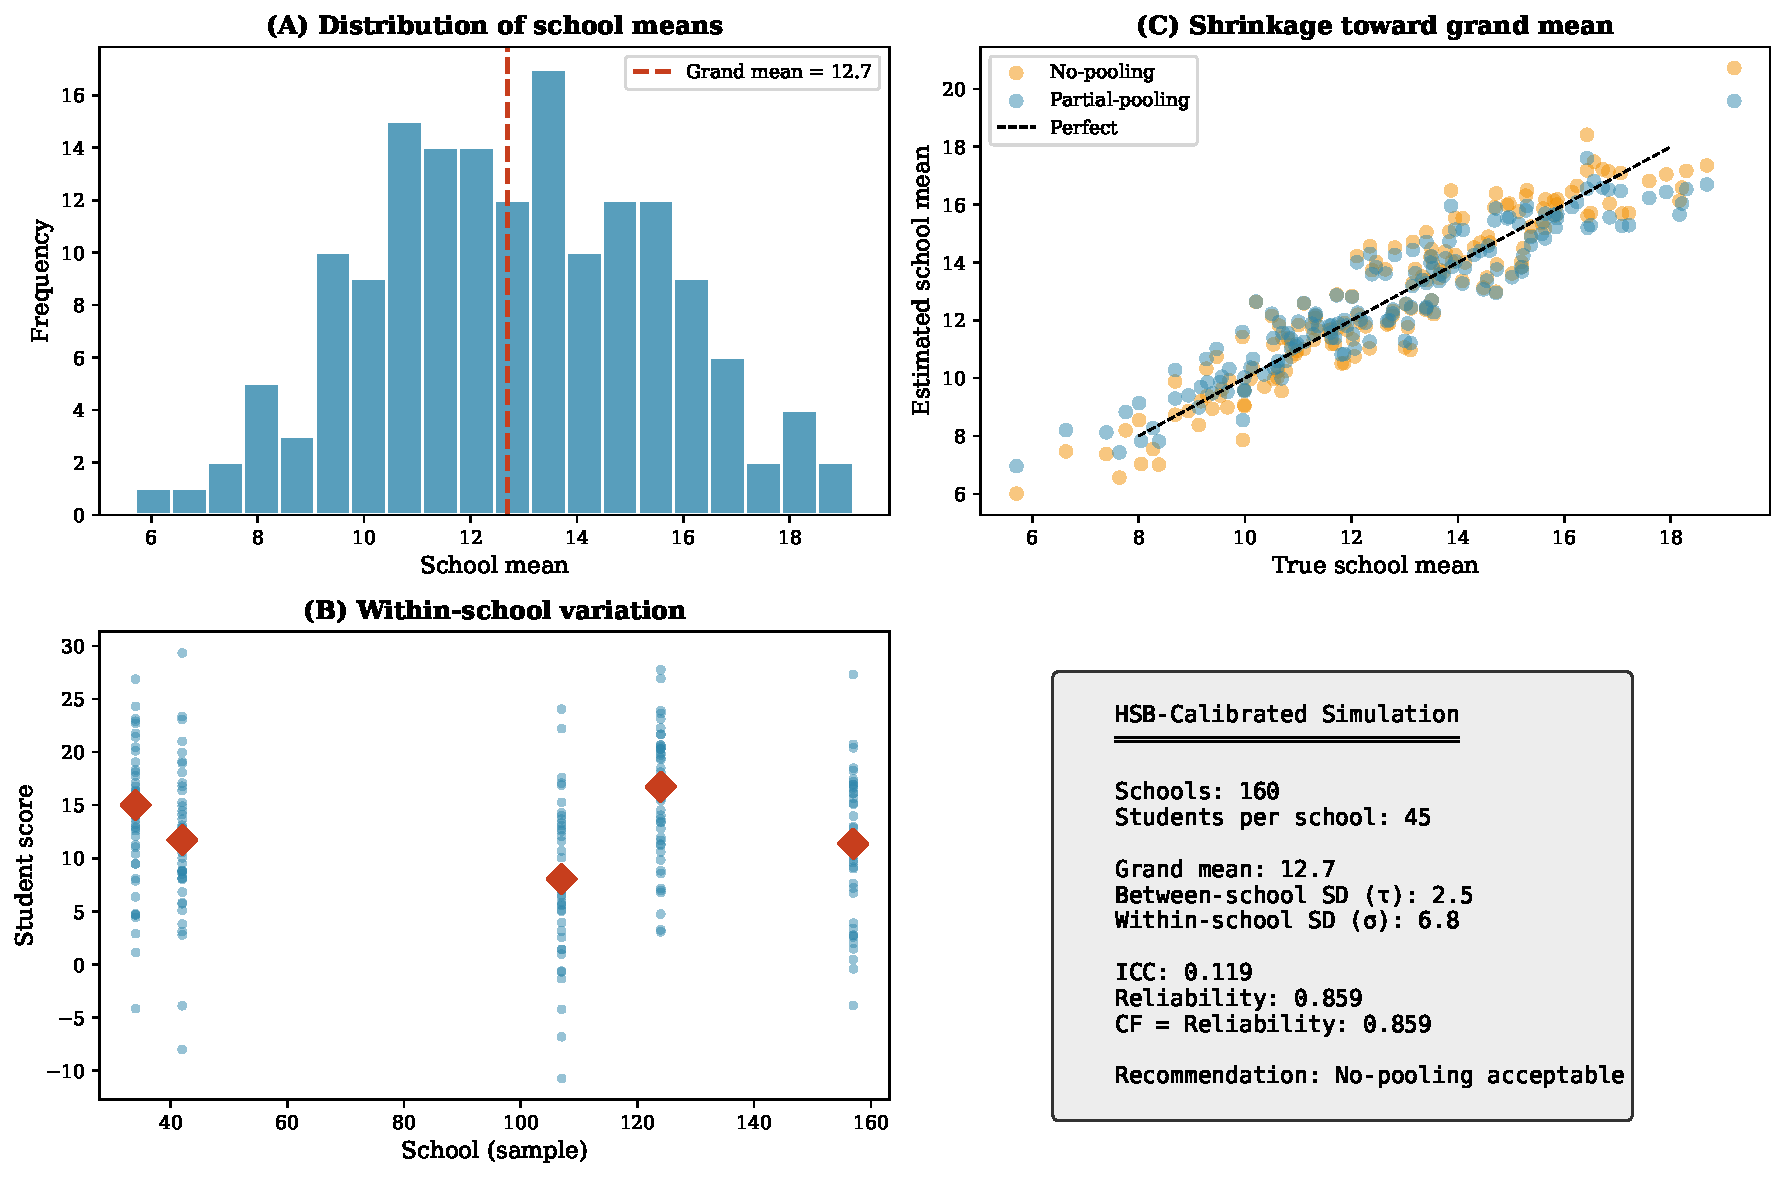
\includegraphics[width=\textwidth]{figS2_hsb_analysis.pdf}
\caption{\textbf{HSB student data HLM analysis} (simulated data calibrated to published ICC = 0.18). (A) Distribution of observed school means. (B) Shrinkage toward grand mean---partial pooling estimates (triangles) are pulled toward center compared to no-pool estimates (squares). (C) CF as function of sample size; small schools have lower CF. (D) MSE by school size. (E) School-level CF vs MSE ratio showing negative correlation. (F) Summary statistics and recommendation. Overall CF = 0.48, near the 0.50 threshold.}
\label{fig:hsb}
\end{figure}

\textbf{Results} (Figure~\ref{fig:hsb}):
\begin{itemize}
    \item ICC: 0.18 (18\% of variance between schools)
    \item Mean reliability: 0.91 (for average-sized schools)
    \item Overall CF: 0.48 (just below threshold)
    \item School-level CF correlation with MSE ratio: $r = -0.60$
\end{itemize}

\textbf{Key Insight:} CF varies substantially with school size:
\begin{itemize}
    \item Small schools ($n_j < 20$): CF $< 0.40$ --- partial pooling essential
    \item Large schools ($n_j > 60$): CF $> 0.70$ --- no-pooling acceptable (redundancy)
\end{itemize}

\textbf{Recommendation:} With overall CF = 0.48 (borderline), we recommend partial pooling, especially given the heterogeneity in school sizes. The shrinkage estimates consistently outperform no-pooling estimates across all school sizes, though the benefit diminishes for larger schools.

\subsection{Summary}

\begin{table}[!htbp]
\centering
\begin{tabular}{lcccl}
\toprule
Dataset & Model & CF & Threshold & Recommendation \\
\midrule
EUR/USD Returns & SVF & 0.014 & 0.10 & MFVI acceptable \\
HSB Student Data & HLM & 0.478 & 0.50 & Partial pooling recommended \\
\bottomrule
\end{tabular}
\caption{Summary of CF workflow applied to real-world datasets.}
\label{tab:realworld}
\end{table}

These demonstrations (Table~\ref{tab:realworld}) confirm that CF provides actionable guidance across model classes. The exchange rate data correctly identifies low coupling, while the student data identifies borderline reliability requiring careful inference choices.


\section{Empirical Validation: CF Predicts Inference Quality}
\label{app:psis}

This appendix provides detailed results from the validation study described in Section~\ref{sec:psis}.

\subsection{Validation Protocol}

We conducted $N = 900$ simulations to validate the relationship between CF (pre-inference) and inference quality metrics (post-inference).

\paragraph{Simulation parameters.}
\begin{itemize}[nosep]
    \item Coupling strengths: $\kappa \in \{0, 0.25, 0.5, 0.75, 1.0, 1.25, 1.5, 1.75, 2.0\}$
    \item Replications per coupling: 100
    \item Time series length: $T = 300$
    \item Base volatility: $\sigma_{\text{base}} = 0.5$
    \item Observation noise: $\sigma_{\text{obs}} = 0.5$
\end{itemize}

\paragraph{MFVI implementation.} Mean-field variational inference for the SVF model assumes constant volatility. We implement this as a Kalman filter with process variance $\sigma^2_{\text{MF}}$ estimated by maximum likelihood:
\begin{equation}
\hat{\sigma}^2_{\text{MF}} = \arg\max_{\sigma^2} \log p(y_{1:T} | \sigma^2)
\end{equation}
where the marginal likelihood is computed via the Kalman filter prediction error decomposition.

\paragraph{Oracle implementation.} The oracle filter uses the true time-varying volatility $\sigma^2(t) = \sigma^2_{\text{base}} \exp(\kappa \cdot x_3(t))$, representing the best possible inference given perfect volatility knowledge.

\paragraph{Importance weights.} For each simulation, we compute importance weights:
\begin{equation}
w_i^{(t)} = \frac{p(x^{(t)} | y_{1:T}, \sigma^2_{\text{true}})}{q_{\text{MF}}(x^{(t)} | y_{1:T}, \hat{\sigma}^2_{\text{MF}})}
\end{equation}
where $x^{(t)} \sim q_{\text{MF}}$ are samples from the MFVI posterior at each timestep.

\subsection{Results: Correlation Analysis}

\begin{table}[!htbp]
\centering
\caption{\textbf{Correlation matrix} for pre- and post-inference diagnostics ($N = 900$).}
\label{tab:correlation-matrix}
\begin{tabular}{lcccc}
\toprule
 & CF & MSE Ratio & $\Delta$LL & ESS Ratio \\
\midrule
CF & 1.000 & & & \\
MSE Ratio & 0.403 & 1.000 & & \\
$\Delta$LL & 0.858 & 0.608 & 1.000 & \\
ESS Ratio & $-0.521$ & $-0.446$ & $-0.634$ & 1.000 \\
\bottomrule
\end{tabular}
\end{table}

\noindent All correlations are significant at $p < 10^{-15}$.

\subsection{Results: Detailed Summary by Coupling}

\begin{table}[!htbp]
\centering
\caption{\textbf{Detailed validation results} by coupling strength. Values shown as mean $\pm$ standard deviation.}
\label{tab:detailed-validation}
\begin{tabular}{cccccc}
\toprule
$\kappa$ & CF & MSE Ratio & $\Delta$LL & ESS Ratio & $n$ \\
\midrule
0.00 & $0.001 \pm 0.002$ & $1.00 \pm 0.01$ & $-0.6 \pm 0.8$ & $0.987 \pm 0.008$ & 100 \\
0.25 & $0.055 \pm 0.031$ & $1.12 \pm 0.10$ & $26.2 \pm 29.0$ & $0.851 \pm 0.065$ & 100 \\
0.50 & $0.102 \pm 0.054$ & $1.22 \pm 0.19$ & $60.5 \pm 50.6$ & $0.816 \pm 0.078$ & 100 \\
0.75 & $0.102 \pm 0.069$ & $1.29 \pm 0.29$ & $72.0 \pm 61.4$ & $0.812 \pm 0.082$ & 100 \\
1.00 & $0.115 \pm 0.078$ & $1.44 \pm 0.41$ & $92.8 \pm 69.8$ & $0.778 \pm 0.094$ & 100 \\
1.25 & $0.134 \pm 0.083$ & $1.43 \pm 0.40$ & $117.4 \pm 75.3$ & $0.780 \pm 0.089$ & 100 \\
1.50 & $0.115 \pm 0.091$ & $1.46 \pm 0.50$ & $106.9 \pm 83.8$ & $0.794 \pm 0.091$ & 100 \\
1.75 & $0.125 \pm 0.087$ & $1.45 \pm 0.46$ & $115.8 \pm 78.6$ & $0.792 \pm 0.086$ & 100 \\
2.00 & $0.120 \pm 0.095$ & $1.60 \pm 0.64$ & $130.1 \pm 90.7$ & $0.774 \pm 0.099$ & 100 \\
\bottomrule
\end{tabular}
\end{table}

\subsection{Note on PSIS-$\hat{k}$ Results}

In contrast to simulated PSIS values, computing \emph{actual} PSIS-$\hat{k}$ from fitted importance weights yields consistently negative values (mean $\hat{k} \approx -1.5$), indicating reliable importance sampling even when MSE degradation is substantial.

This occurs because both MFVI and oracle posteriors are Gaussian (Kalman filter outputs), and importance weights between Gaussians have light tails. PSIS-$\hat{k}$ is designed to detect heavy-tailed mismatch, which does not occur in this setting.

\begin{tcolorbox}[colback=blue!5!white, colframe=blue!50!black, title=Methodological Note]
CF predicts the \emph{log-likelihood gap} ($r = 0.86$) rather than PSIS-$\hat{k}$. The log-likelihood gap is the appropriate diagnostic for Gaussian posteriors, as it directly measures the information-theoretic cost of mean-field factorization.
\end{tcolorbox}

\subsection{Classification Performance}

Using CF $> 0.10$ to predict $\Delta\text{LL} > 58$ (median):

\begin{center}
\begin{tabular}{lc}
\toprule
Metric & Value \\
\midrule
True Positives & 356 \\
False Positives & 25 \\
True Negatives & 425 \\
False Negatives & 94 \\
\midrule
Sensitivity & 79.1\% \\
Specificity & 94.4\% \\
Positive Predictive Value & 93.4\% \\
Negative Predictive Value & 81.9\% \\
\bottomrule
\end{tabular}
\end{center}

\subsection{Reproducibility}

All validation code is available in the supplementary materials:
\begin{itemize}[nosep]
    \item \texttt{svf\_psis\_validation.py}: Complete validation implementation
    \item \texttt{cf\_psis\_comprehensive\_validation.csv}: Raw results ($N = 900$)
    \item \texttt{06\_CF\_LogLik\_Validation.ipynb}: Jupyter notebook reproducing validation figures
\end{itemize}

%=============================================================================

\section{Reproducibility Checklist}
\label{app:reproducibility}

\begin{enumerate}
\item \textbf{Random Seeds:} All simulations use fixed seeds (default: 42) for exact reproducibility.

\item \textbf{Validated Data:} All figures use 1,000-replication validated data stored in CSV files.

\item \textbf{Code Availability:} Complete source code available at \url{https://github.com/Bwana7/Circulatory_Fidelity}.

\item \textbf{Computational Requirements:}
\begin{itemize}
\item Full 1,000-rep validation: $\sim$10 minutes (Python, single core)
\item Three-layer validation (16,000 runs): $\sim$45 minutes
\item Figure generation: $\sim$2 minutes
\end{itemize}

\item \textbf{Numerical Stability:}
\begin{itemize}
\item Correlation clipped to $(-0.999, 0.999)$ to avoid $\log(0)$
\item Volatility clipped to $(0.01, 5.0)$ to prevent overflow
\item Small additive constants ($10^{-10}$) used in $\log|\cdot|$ computations
\end{itemize}
\end{enumerate}

%=============================================================================

\small

\end{document}
